\documentclass{article}    
\usepackage[utf8]{inputenc}
\usepackage[italian]{babel}
\usepackage{setspace}
\usepackage{listings}
\usepackage{xcolor}
\usepackage{natbib}
\usepackage{graphicx}
\usepackage{float}
\usepackage{geometry}
\geometry{a4paper, top=3cm, bottom=3cm}




\begin{document}
\onehalfspacing
\include{Capitoli/titolo}
\tableofcontents
\newpage
\listoffigures
\lstset{language=Matlab}
\lstset{frameround=fttt}
\include{Capitoli/AttivitàPreliminare}
\section{Analisi della macchina}
\subsection{Introduzione}
I compressori alternativi possono essere caratterizzati tramite diversi diagrammi (T-s, p-V, h-s), il più interessante per l'applicazione in esame è il diagramma indicato p-V. \\
\\
Il diagramma indicato è un diagramma che ha la pressione in ordinata e il volume in ascissa.
Non è un diagramma termodinamico, perché il volume in ascissa non è il volume specifico del fluido, ma è il volume (in $m^3$) del cilindro spazzato dal pistone durante il suo funzionamento. (Non si definisce in maniera univoca lo stato termodinamico del fluido).\\
Questo diagramma spiega semplicemente come cambia la pressione all’interno della macchina. 
\paragraph{Caso ideale}Il diagramma è compreso tra un volume minimo (stantuffo in PME) e un volume massimo (stantuffo in PMI), tra PME e PMI si identifica la cilindrata, ovvero il volume spazzato dal pistone. \\
\begin{figure}[h]
    \centering
    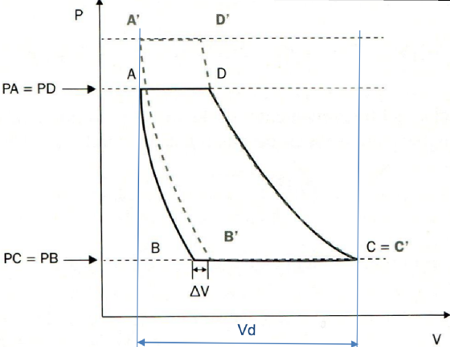
\includegraphics{Immagini/CasoIdeale.png}
    \caption{Andamento diagramma p-V caso ideale}
    \label{fig:CasoIdeale}
\end{figure}
\\
Nel punto di fine aspirazione C, inizia la compressione, il volume a disposizione del fluido inizia a ridursi e la pressione inizia ad aumentare, fino a quando la pressione all’interno del cilindro diventa uguale (caso ideale) alla pressione esterna, cioè quella all'interno del condotto di mandata.  Si arriva così al punto D, dove la pressione all’interno del cilindro è uguale alla pressione all’esterno, la valvola automatica si apre istantaneamente e avviene il trasferimento del fluido da dentro al cilindro alla mandata (non cambiano le caratteristiche del fluido perché non si ha più lo stantuffo che lo comprime, semplicemente viene spinto fuori dal pistone, su un diagramma T-s il tratto DA sarebbe un punto, perché non avviene una trasformazione termodinamica). \\
Si arriva dunque al punto A, lo stantuffo inverte la corsa, il volume a disposizione comincia ad aumentare, la pressione inizia a diminuire (espansione del gas rimanente dentro il cilindro) e la valvola di mandata si chiude immediatamente. Quando la pressione all'interno del cilindro diventa uguale a quella di aspirazione, la valvola si apre e il tratto di  corsa da B verso C vede il gas entrare dentro il cilindro (anche in questo caso nel piano T-s il punto B coincide con C). \\
\\
Ci sono caratteristiche di questo diagramma che dipendono dalla geometria del compressore (volume minimo e cilindrata) e altre caratteristiche che non dipendono prettamente dalla macchina, ma dipendono da come questa sta lavorando.\\
\\
Se la pressione di mandata diventa più alta (D’ e A’), il diagramma indicato cambia a parità di compressore. Si deve raggiungere una pressione più elevata rispetto a prima per aprire la valvola. Essendo la pressione più elevata, serve una corsa più lunga per diminuirla fino al livello di prima e quindi l’aspirazione inizia dopo. 
Come risultato finale si ottiene la riduzione della corsa per l’aspirazione all’aumentare della pressione di mandata. All’aumentare della pressione di mandata si riducono sempre di più i tratti orizzontali del diagramma. (Se si ha una pressione di mandata così elevata che tutta la corsa utile del pistone non riesce a creare una depressione tale da aprire le valvole, il compressore diventa una molla pneumatica). \\
Ha senso quindi utilizzare il compressore per un certo valore della pressione di mandata. \\
\\
Si traducono questi concetti in equazioni.\\
\\
Si definisce il coefficiente di volume ideale come:
\begin{equation}
 \lambda_{Vi}=\frac{m_C-m_B}{\rho_{AS}\cdot V_d}=\frac{\mbox{massa aspirata}}{\mbox{massa ideale, massimo fluido che si può introdurre nel cilindro}}.
\end{equation}
La portata massica ideale la si può esprimere come portata massica aspirabile corretta dal coefficiente volumetrico ideale, moltiplicata per i giri al secondo $\dot{m}=\lambda_{Vi}\cdot\rho_{AS}\cdot\ V_d\cdot\frac{n}{60}\ .$\\
\\
Si definisce coefficiente di volume nocivo come:  $\varepsilon=\frac{V_A}{V_d}$ .\\
\\
Il rapporto tra la pressione di mandata e la pressione di aspirazione viene chiamato rapporto di compressione $\frac{V_B}{V_A}=\left(\frac{p_B}{p_A}\right)^\frac{1}{k}=\beta^\frac{1}{K}$. Si ottiene quindi $\lambda_{Vi}=1-\varepsilon\left(\beta^{1/k}-1\right)$.\\
\\
All’aumentare di $\beta$, $\lambda_{Vi}$ diminuisce, che è esattamente quello che si è detto prima commentando il diagramma indicato. La massa di aria aspirata diminuisce all’aumentare della pressione di mandata e quindi del $\beta$ (tenendo implicitamente costante la pressione di aspirazione). Ne consegue che più grande è il volume minimo, più grande è $\varepsilon$ (a parità di cilindrata), il quale essendo negativo fa diminuire il $\lambda_{Vi}$ a parità di $\beta$, da qui il termine nocivo (perché minore è la portata che il compressore può erogare). \\
Chiaramente più è grande il volume minimo, più gas rimane intrappolato a fine corsa e quindi dovrà espandere maggiormente per aprire la valvola di aspirazione, sottraendo parte della corsa utile del pistone.
\paragraph{Caso reale}
In questo caso bisogna abbandonare l'ipotesi di completa idealità nel funzionamento supposta prima, ovvero che la valvola di mandata si apra quando la pressione all’interno del cilindro è uguale a quella esterna. \\
Solo con pressioni diverse, quindi forze diverse (non equilibrate), la valvola si apre. \\
\\
Si vede che sono presenti due rapporti di compressione. Il rapporto esterno è il rapporto che si instaura tra la pressione nel condotto di mandata e la pressione nel condotto di aspirazione, ed è quello che si deve considerare.\\ 
\\
Per quanto detto prima però per aprire le valvole il cilindro deve avere delle pressioni diverse rispetto a quelle nei condotti. Quindi, si viene a definire un rapporto di compressione interno.
\begin{figure}[h]
    \centering
    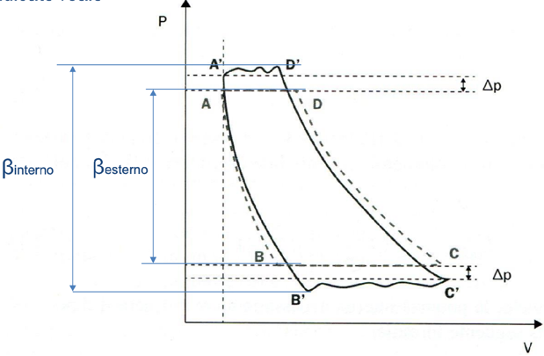
\includegraphics{Immagini/CasoReale.png}
    \caption{Andamento diagramma p-V caso reale}
    \label{fig:CasoReale}
\end{figure}
\\
Partendo da C (C’) come prima, il fluido subisce una compressione per cui la pressione aumenta fino a D’, che si trova a pressione maggiore rispetto ad A. Si nota inoltre che D’ è leggermente più alto rispetto ad A’ perché la valvola rappresenta una perdita di carico concentrata e il fluido attraversandola diminuisce la sua pressione (l’andamento è oscillatorio per motivi legati alla dinamica del gas). \\
Il fluido si ferma ad una pressione leggermente più alta rispetto a quella di mandata (A’-A).\\ Parlando di aria, il moto sarà sicuramente turbolento e le perdite concentrate in tale regime dipendono dal quadrato della velocità del flusso (o dalla portata). La velocità del fluido attraverso la valvola non dipende dalla differenza di pressione (quella è una conseguenza), ma dalla velocità dello stantuffo che spinge fuori il gas.\\
Quindi, le perdite di carico dipendono dalla velocità al quadrato, la velocità dipende dal moto dello stantuffo, quando lo stantuffo va verso il PME, va verso velocità nulla e quindi espelle sempre più lentamente il gas attraverso la valvola, evidenziando perdite di carico sempre più piccole. È per questo che la differenza tra dentro e fuori il cilindro è una differenza che si riduce (andamento decrescente D’-A’). \\
Siccome il  moto del cilindro è molto veloce, nel momento in cui la valvola è aperta non si ha il tempo a sufficienza per uniformare le pressioni tra A’ e A, per cui all’interno del cilindro rimane una pressione più alta della pressione di mandata ($\Delta p_{A'-A}$) da cui inizia direttamente la fase di espansione. \\
\\
Per la fase aspirazione avviene esattamente la stessa cosa, all’interno del cilindro la pressione dovrà essere minore rispetto a quella di aspirazione in modo tale da permettere alla valvola di aprirsi. Durante la fase di ingresso del gas si avrà sempre, all’interno del cilindro, una pressione differente rispetto a quella di aspirazione che va aumentando verso il punto morto inferiore, perché si riduce la velocità di scorrimento dello stantuffo e quindi le perdite di carico. \\
\\
Arrivando al punto C’, appena sotto al punto C, per lo stesso motivo esposto prima, il processo è istantaneo e non c’è tempo per le pressioni di stabilizzarsi. \\
\\
Il diagramma reale, quindi è quello rappresentato in figura, che permette di definire due rapporti di compressione: uno interno ed uno esterno al cilindro.\\
\\
La corsa utile del caso reale si è ridotta rispetto al caso ideale, per cui il coefficiente di riempimento sarà minore rispetto a quello ideale. Le fasi di compressione ed espansione rimangono sostanzialmente delle isoentropiche anche nel ciclo indicato reale. \\
\\
Si capisce immediatamente che mentre il ciclo indicato ideale è definito da delle equazioni che permettono di trovare univocamente i punti di interesse, trovare i punti reali è molto più complicato e i calcoli dovranno essere molto più sofisticati. 
\subsection{Grandezze caratteristiche compressore}

\underline{Dati}: \\
Fluido: aria. \\
Pressione di mandata: $p_M$ = 10 bar.\\
Alesaggio: d = 55 mm.\\
Corsa: s = 42 mm.\\
Cilindrata: $V_d$ = 200 $cm^3$.\\
Velocità di rotazione della manovella: n = 1540 giri/min.\\
Diametro Volano: D = 300 mm ($d_{2m}$= 287 mm). \\
Numero cilindri: N = 2.\\
Stadi di compressione: 1. \\
Per i calcoli si suppone un coefficiente di volume nocivo $\varepsilon$ = 0,05.\\
Essendo il fluido aria il rapporto calore specifico a pressione costante e calore specifico a volume costante è k = 1,4 .\\
Si assume una temperatura di aspirazione pari alla temperatura ambiente T = 293 K (20$^\circ$ C).\\
L’aria può essere considerata “idealmente” come un gas perfetto e pertanto si assumere la costante dei gas R = 287 J/kgK .
\subsubsection{Portata d'aria}
Come descritto nell’introduzione la portata di aria compressa erogata dal compressore è: 
\begin{equation}
    \varepsilon = 0.05.
\end{equation}
\begin{equation}
    \beta=p_M/p_A=11/1=11
\end{equation}
\begin{equation}
    k=1.44
\end{equation}
\begin{equation}
    \lambda_{Vi}=1-\varepsilon\left(\beta^{1/k}-1\right)=0.77
\end{equation}
\begin{equation}
    \rho_{AS}=\frac{p_A}{RT_A}=1.19\ kg/m^3
\end{equation}
\begin{equation}
    \dot{m}=\lambda_{Vi}\cdot\rho_{AS}\cdot\ V_d\cdot\frac{n}{60}=4.7\cdot{10}^{-3}\ kg/m^3
\end{equation}
\subsubsection{Temperatura di mandata}Si può considerare che un gas compresso aumenti la propria temperatura secondo l’equazione dell’isoentropica e di conseguenza nascono alcuni problemi:
\begin{itemize}
    \item Difficoltà nella scelta materiali con cui deve essere realizzato il compressore (tenute stantuffo-cilindro). 
    \item Difficoltà nella lubrificazione (non si possono ammettere particelle di lubrificante in sospensione nel fluido, per questo vengono utilizzati dei segmenti che impongono vincoli sulla temperatura).
\end{itemize}
Questi problemi legati alla temperatura intervengono già da un rapporto di compressione da 5 a 8. Tuttavia, il motivo per il quale il rapporto di compressione del sistema in esame può spingersi fino a 11 è perché, essendo una macchina adibita al settore hobbistico, l’affidabilità richiesta è minore rispetto ad una adibita al settore industriale.\\
\\
Per calcolare la temperatura di mandata si utilizzano le relazioni termodinamiche dell’isoentropica: 
\begin{equation}
    T_M=T_A\ \beta^\frac{k-1}{k}
\end{equation}
sostituendo con i valori, si ottiene $T_M=581,3\ K=308,3^\circ C$.\\
\\
È stato ricavato nell’ambiente di programmazione Matlab l’andamento della temperatura di mandata in funzione del rapporto di compressione $\beta$. 
\begin{figure}[h]
    \centering
    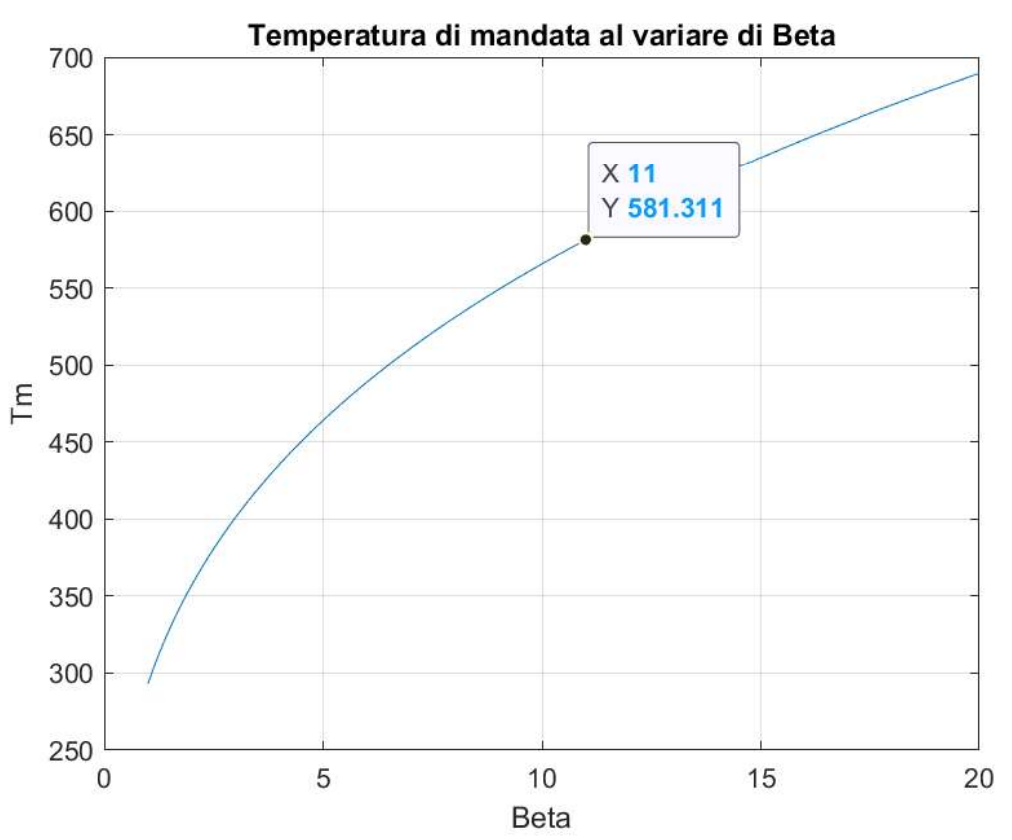
\includegraphics[scale=0.6]{Immagini/GraficoTmBeta.png}
    \caption{Andamento della temperatura di mandata in funzione di $\beta$}
    \label{fig:GraficoTmBeta}
\end{figure}
\\
\\
\begin{lstlisting}[frame=trBL]
%%Dati
Ta=293;                  %Temperatura di aspirazione
k=1.4;                   %Coefficiente isoentropica
eps=0.05;                %Coefficiente volume nocivo
Cil=0.0002;              %Cilindrata[metri cubi]
Pa=101325;               %Pressione Aspirazione[Pa]
Pm=1114575;              %Pressione Mandata[Pa]

%Grafico Temperatura di Mandata%
Beta=1:0.1:20;          %Definizione di beta
Tm=Ta*Beta.^((k-1)/k);  %Calcolo parametro controllato 
plot(Beta,Tm);
xlabel('Beta'),ylabel('Tm'),title('Temperatura di mandata al variare 
      di Beta'),grid on;
\end{lstlisting}
\subsubsection{Diagramma indicato p-V}In conclusione, alla trattazione riguardante l’analisi della macchina, viene di seguito rappresentato il diagramma indicato p-V. \\
Il grafico sarà costituito da 2 trasformazioni isobare, una a $p_M$ e una a $p_A$ e da due isoentropiche, una di espansione e una di compressione. \\
Il ciclo è ottenuto mediante codice all’interno dell’ambiente di programmazione Matlab. 
\begin{figure}[h]
    \centering
    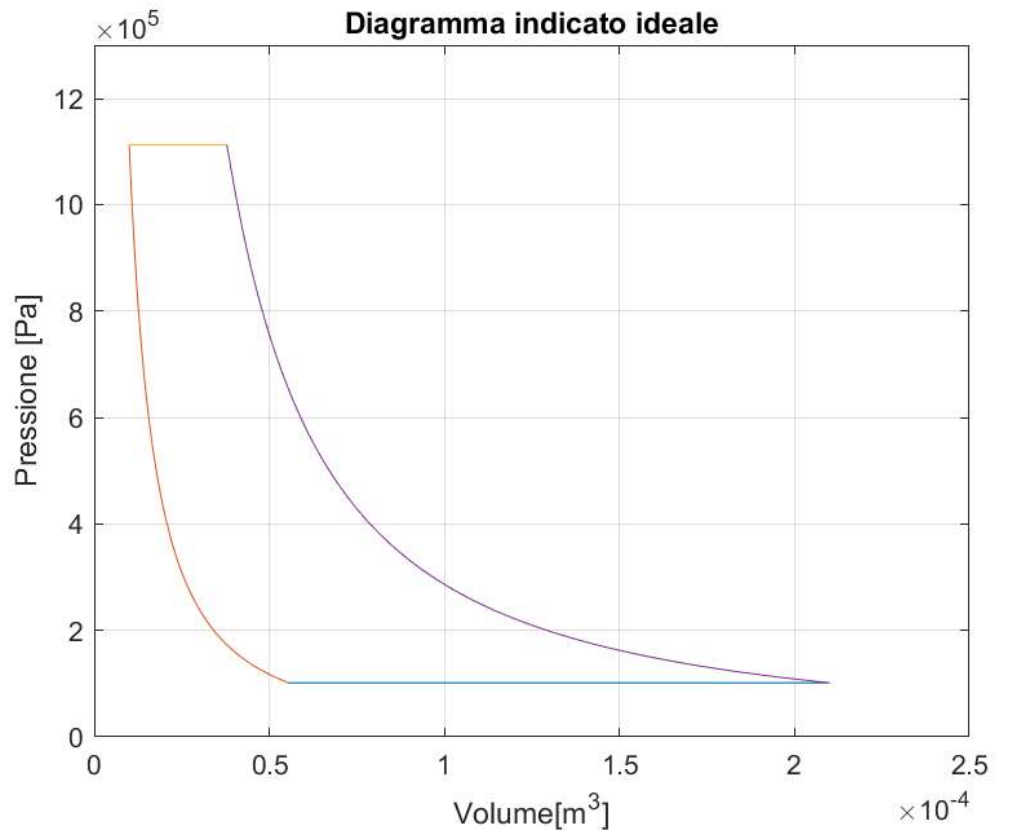
\includegraphics[scale=0.6]{Immagini/GraficopV.png}
    \caption{Andamento diagramma p-V compressore}
    \label{fig:GraficopV}
\end{figure}
\\
\\
\\
\\
\begin{lstlisting}[frame=trBL]
%%Dati
Ta=293.15;              %Temperatura di aspirazione
K=1.4;                  %Coefficiente isentropica
eps=0.05;               %Coefficiente volume nocivo
Cil=0.0002;             %Cilindrata
Pa=101325;               %Pressione Aspirazione
Pm=1114575;              %Pressione Mandata

%%Grandezze Ricavate
Vpmi=Cil*(1+eps);                    %Volume punto morto inferiore
Vpms=Cil*eps;                        %Volume punto morto superiore

%Grafico Ciclo ideale compressore%

%Compressione del fluido
Pciclo=Pa:500:Pm;            %Definizione vettore pressioneda Pa a Pm
Vciclo=(Pa.^(1/K))*(Pciclo.^(-1/K))*Vpmi; %Calcolo Volume 
                                          %in fase di compressione
%Espulsione del fluido
Vespuls=linspace(Vpms,3.79067*10^-5,5);  %Definizione vettore Volume 
                                         %Espulsione
%Espansione
Vcicloesp=(Pm.^(1/K))*(Pciclo.^(-1/K))*Vpms;  %Calcolo Volume 
                                              %Espansione
%Aspirazione
Vaspirato=linspace(5.54437*10^-5,Vpmi,5);  %Definizione vettore Volume 
                                           %Aspirazione
plot(Vaspirato,Pcicloasp);
hold on
plot(Vcicloesp,Pciclo);
hold on 
plot(Vespuls,Pcicloesp);
hold on;
plot(Vciclo,Pciclo);
xlabel('Volume[m^3]'),ylabel('Pressione [Pa]'),title
       ('Diagramma indicato ideale'),ylim([0 13*10^5]),grid on;
\end{lstlisting}


\section{Analisi dei carichi del cinematismo}
Il meccanismo biella manovella è uno dei cinematismi più noti all’interno della meccanica applicata. \\
Il suo funzionamento è stato studiato negli anni attraverso diversi libri di testo. \\
\begin{figure}[h]
    \centering
    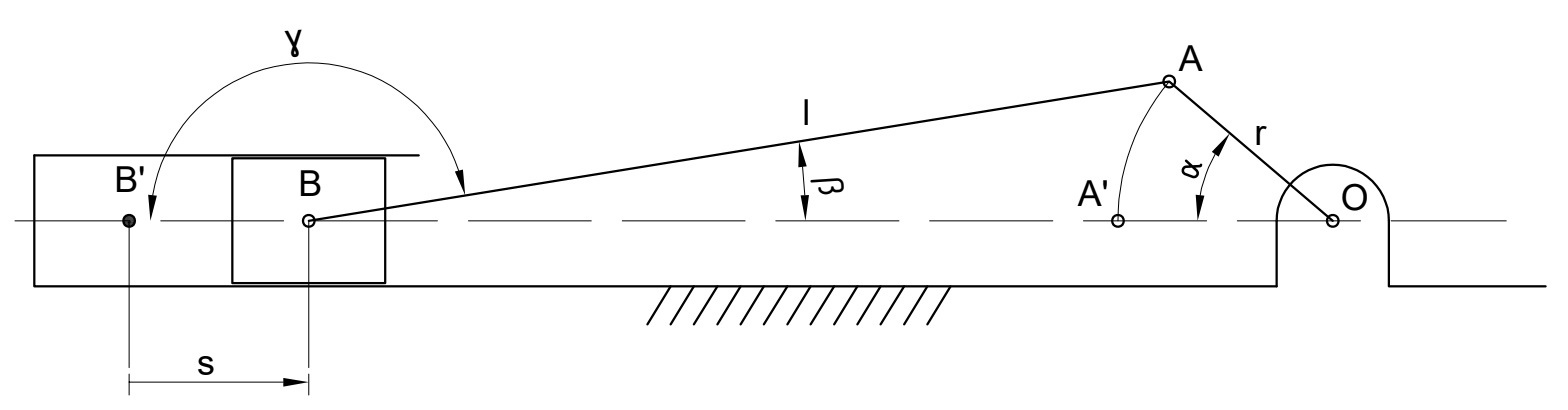
\includegraphics[scale=0.4]{Immagini/Cinematismo.png}
    \caption{Schema cinematismo biella-manovella}
    \label{fig:Cinematismo}
\end{figure}
\\
Si consideri il manovellismo in una posizione generica. \\
Nella figura mostrata si distinguono:
\begin{itemize}
   \item l lunghezza di biella 
   \item r raggio di manovella 
   \item $\alpha$ angolo di manovella 
	\item $\gamma$ angolo di inclinazione della biella 
	\item s spostamento generico del piede di biella 
\end{itemize}
\subsection{Andamento dello spostamento in funzione dell'angolo di manovella}
Si definisce la corsa s del pistone lo spostamento punto B da un punto morto B’, a cui corrisponde la posizione A’ del punto A.\\
Si indichi con $\alpha$ l’angolo che AO forma con il raggio AO’ e con l’angolo $\gamma$, l’angolo che AB forma con l’asse del moto di B. \\
Si indichi con r la lunghezza OA e con l la lunghezza AB.\\
Proiettando la spezzata BAO sull’asse del moto di B si ottiene:
\begin{equation}
    s=l+r+l\cos\left(\gamma\right)-r\cos\left(\alpha\right).
\end{equation}
Proiettando poi la stessa spezzata sulla direzione normale alla precedente eapplicando il teorema dei seni, si ottiene:
\begin{equation}
    l\sin\left(\gamma\right)=r\sin\left(\alpha\right)
\end{equation}
se si indica con $\lambda=\frac{l}{r}$ , diventa 
\begin{equation}
    \sin\left(\gamma\right)=\frac{1}{\lambda}\cdot\sin\left(\alpha\right)
\end{equation}
tenendo conto che $\gamma>\pi/2$
\begin{equation}
    \cos\left(\gamma\right)=-\sqrt{1-\frac{1}{\lambda^2}\cdot\left(\alpha\right)}.
\end{equation}
L’espressione di s diventa quindi 
\begin{equation}
    s=r\cdot\left[1-\cos\left(\alpha\right)+\lambda-\sqrt{\lambda^2-\sin^2\left(\alpha\right)}\right]
    \label{spostamento}
\end{equation}
\\
il cui grafico, in funzione di $\alpha$, è stato ricavato in ambiente Matlab.
\begin{figure}[h]
    \centering
    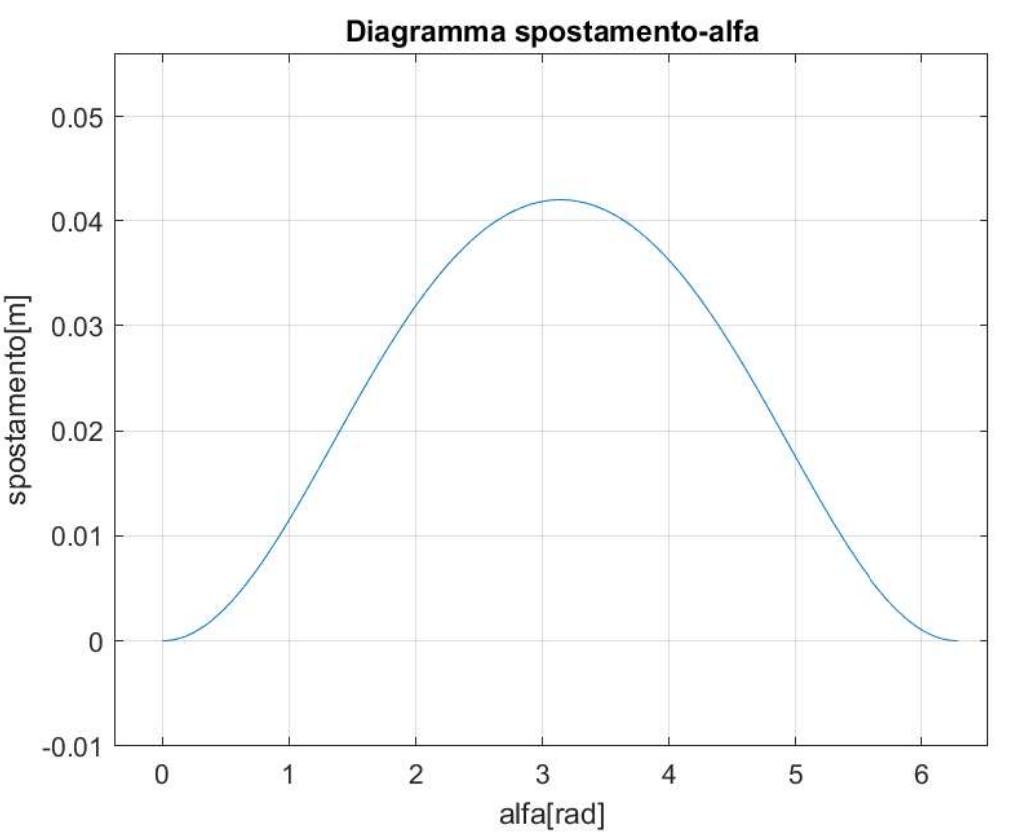
\includegraphics[scale=0.5]{Immagini/GraficoSpostamento.png}
    \caption{Andamento spostamento pistone in dunzione di $\alpha$}
    \label{fig:GraficoSpostamento}
\end{figure}
\begin{lstlisting}[frame=trBL]
%Dati
Ta=293.15;               %Temperatura di aspirazione [K]
k=1.4;                   %Coefficiente isentropica
eps=0.05;                %Coefficiente volume nocivo
Cil=0.0002;              %Cilindrata
Pa=101325;               %Pressione Aspirazione
Pm=1114575;              %Pressione Mandata
r=21*10^-3;              %raggio manovella
l=85*10^-3;              %lunghezza biella
n_cil=2;                 %Numeri cilindri
corsa=0.042;             %corsa cilidri
d=0.055;                 %Alesaggio

%Grandezze Ricavate
Vpmi=Cil*(1+eps);                        %Volume punto morto inferiore
Vpms=Cil*eps;                            %Volume punto morto superiore
lamda=l/r;                               %rapporto biella-manovella
omega=(2*pi*n)/60;                       %Velocita manovella[rad/s]
Vcilindro=(pi*d^2/4)*corsa;              %Cilindrata
Apist=d^2*pi/4;                          %Area pistone

%Grafico spostamento al variare di alfa
alfa=linspace(0,2*pi,6296);      %vettore da 0 a 2pi con 
                                 %6296 volte un radiante
spostamento=r*(1-cos(alfa)+lambda-sqrt(lambda^2-sin(alfa).^2));
plot(alfa,spostamento);
xlabel('alfa[rad]'),ylabel('spostamento[m]'),
        title('Diagramma spostamento-alfa'),
        ylim([ 0.06]),grid on,xlim([0 2*pi]);
\end{lstlisting}
\subsection{Andamento del volume in funzione dell'angolo di manovella}
Considerando quanto ottenuto prima, moltiplicando lo spostamento per la sezione del pistone e aggiungendo il volume nocivo intrappolato a fine compressione, si ottiene l’andamento del volume in funzione dell’angolo di manovella:
\begin{equation}
    V=V_{\mathrm{nocivo}}+s\cdot\frac{\pi d^2}{4}
\end{equation}
\begin{figure}[h]
    \centering
    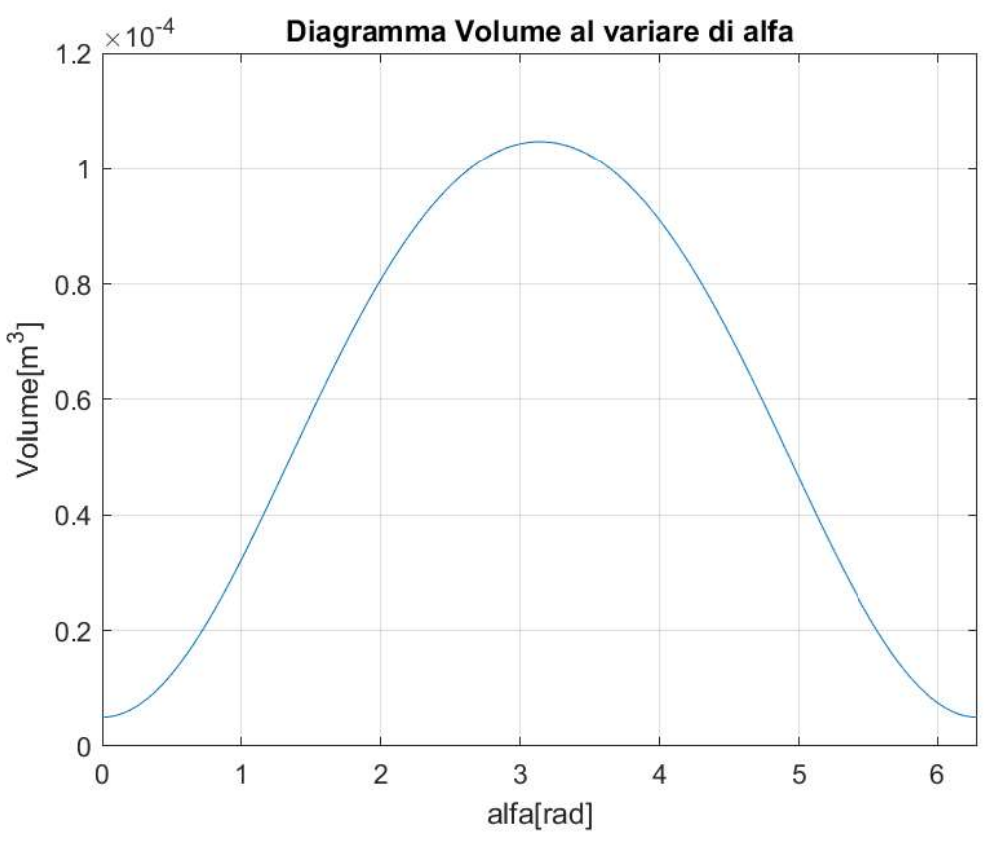
\includegraphics[scale=0.5]{Immagini/GraficoVolume.png}
    \caption{Andamento volume spazzato in funzione di $\alpha$}
    \label{fig:GraficoVolume}
\end{figure}
\begin{lstlisting}[frame=trBL]
%Volume cilindro al variare di alfa%
Vnocivo=eps*Vcilindro;
Vist=Vnocivo+(pi*d^2/4)*spostamento; %volume all'interno di un
                                     %unico cilindro in funzione dello 
                                     %spostamento
plot(alfa,Vist);
xlabel('alfa[rad]'),ylabel('Volume[m^3]'),
      title('Diagramma Volume al variare di alfa'),
      grid on,xlim([0 2*pi]);
\end{lstlisting}
\subsection{Andamento della pressione in funzione dell'angolo di manovella}
Per analizzare l’andamento della pressione all’interno del cilindro, in funzione di $\alpha$, si ipotizza di considerare trasformazioni di compressione ed espansione isoentropiche (nell’ipotesi di aria come gas perfetto).\\
Vale quindi:
\begin{equation}
    pV^k=\mathrm{cost}.
\end{equation}
Questa equazione può essere espressa in funzione di due stati del sistema, uno incognito (pV) ed uno noto ($p_0V_0$).
\begin{equation}
    pV^k=p_0V_0^k.
\end{equation}
Da cui si ricava:
\begin{equation}
    p=p_0\left(\frac{V_0}{V}\right)^k.
\end{equation}
Nel caso di espansione, lo stato noto è lo stato in cui il volume $V_0=V_{\mathrm{nocivo}}$ e quindi la pressione $p_0=p_M$.\\
Si avrà quindi:
\begin{equation}
    p=p_M\left(\frac{V_{\mathrm{nocivo}}}{V}\right)^k
\end{equation}
Nel caso di compressione, invece, lo stato noto sarà quello in cui la pressione $p_0=p_A$ e il volume sarà il volume massimo all’interno del cilindro
$V_0=V_{\mathrm{nocivo}}+V_{\mathrm{cilindro}}$.\\
Per cui:
\begin{equation}
    p=p_A\left(\frac{V_{\mathrm{nocivo}}+V_{\mathrm{cilindro}}}{V}\right)^k
\end{equation}
Avendo precedentemente ricavato l’andamento del volume in funzione dell’angolo di manovella, sempre in ambiente Matlab è stato possibile ottenere il grafico rappresentante la pressione in funzione del medesimo angolo.\\
\begin{figure}[h!]
    \centering
    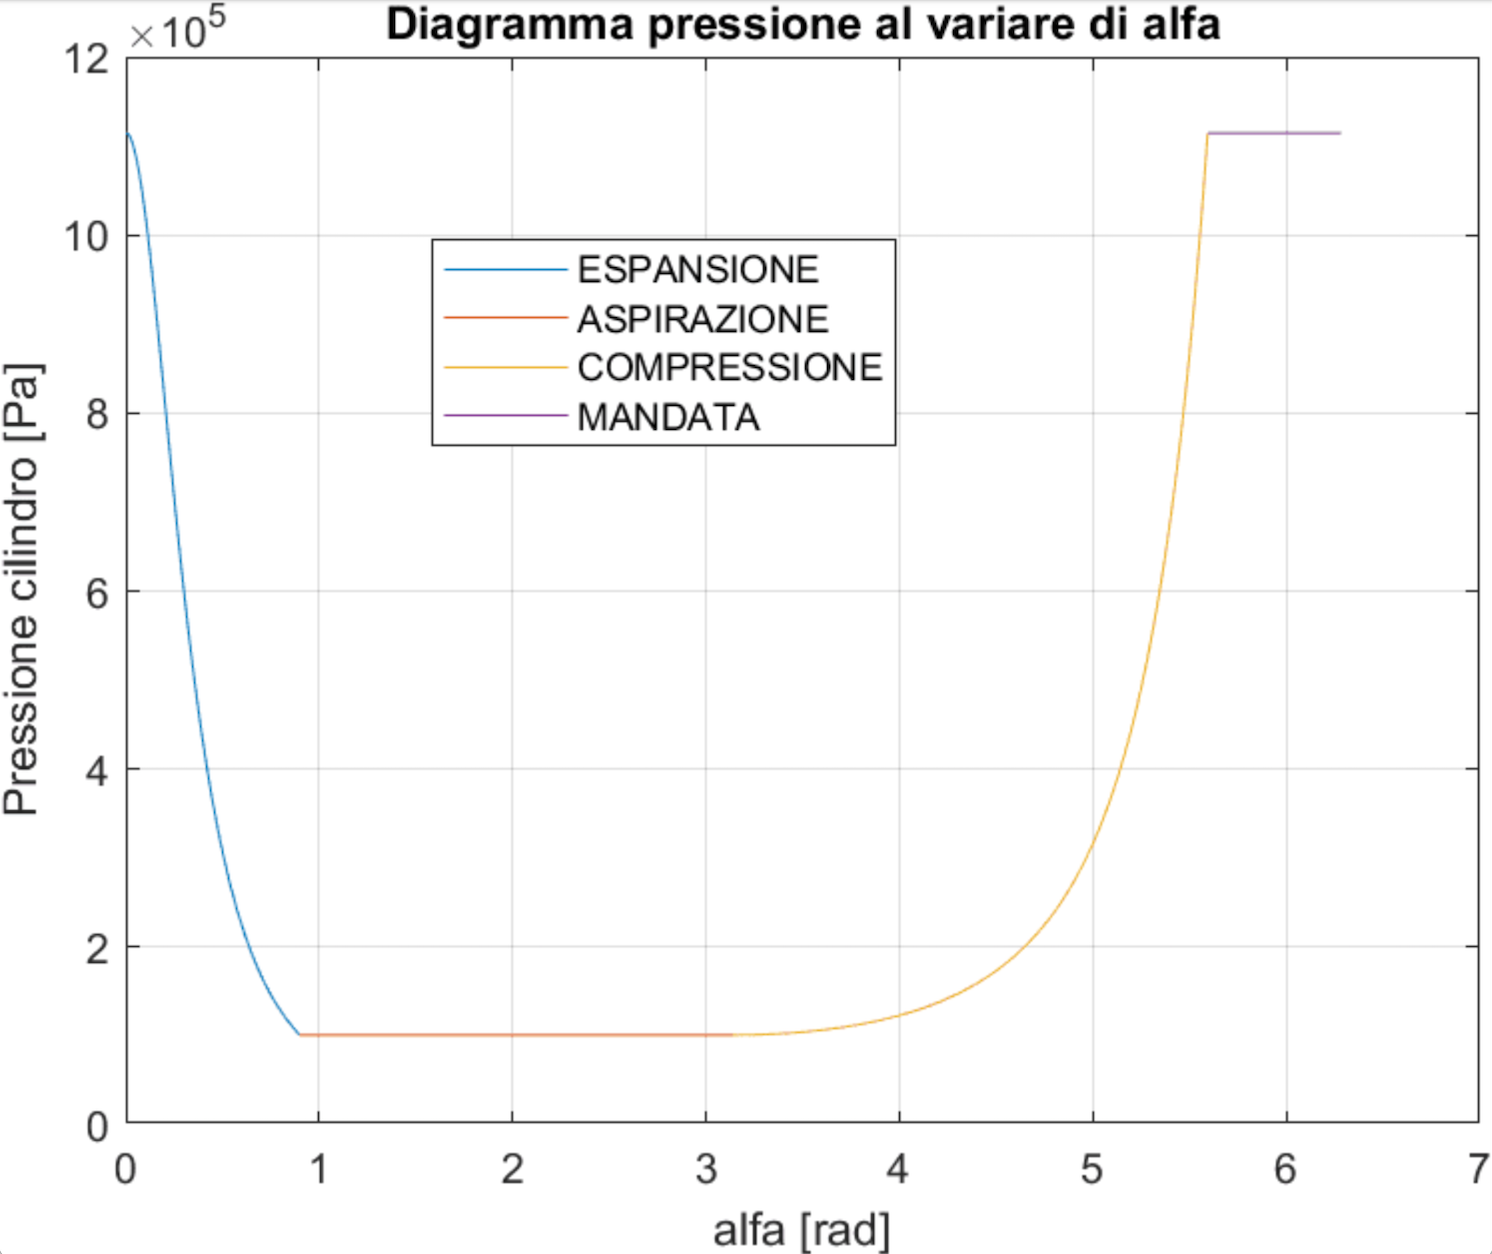
\includegraphics[scale=0.35]{Immagini/GraficoPressione.png}
    \caption{Andamento della pressione in funzione di $\alpha$}
    \label{fig:GraficoPressione}
\end{figure}
\begin{lstlisting}[frame=trBL]
%grafico pressione al variare di alfa

%espansione
alfaesp=linspace(0,0.8989, )
spostamentoesp=r*(1-cos(alfaesp)+lambda-
               sqrt(lambda^2-sin(alfaesp).^2))
Vistesp=Vnocivo+(pi*d^2/4)*spostamentoesp
pressioneesp=Pm*(Vnocivo*((Vistesp).^-1)).^k;
plot(alfaesp,pressioneesp);
hold on

%aspirazione
ya=Pa*ones(1,737);
xa=linspace(0.8989,pi,2000);
plot(x,y);
hold on

%compressione
alfacomp=linspace(pi,5.5934,758)
spostamentocomp=r*(1-cos(alfacomp)+lambda-
                sqrt(lambda^2-sin(alfacomp).^2))
Vistcomp=Vnocivo+(pi*d^2/4)*spostamentocomp
pressionecomp=Pa*((Vnocivo+Vcilindro)*((Vistcomp).^-1)).^k;
plot(alfacomp,pressionecomp)
hold on

%mandata
ym=Pm*ones(1,241);
xm=linspace(5.5934,2*pi,2000);
plot(x,y);
hold on
grid on
xlabel('alfa [rad]'),ylabel('Pressione cilindro [Pa]'),
      title('Diagramma pressione al variare di alfa');
\end{lstlisting}
\newpage
\subsection{Valutazione della massa dei componenti}
Per procedere con l'analisi dei carichi è indispensabile determinare le masse dei principali elementi del cinematismo. Queste possono essere valutate modellando i componenti con un programma di disegno solido (SOLIDWORKS nel nostro caso).
Una volta definita la geometria del pezzo, la funzione "proprietà di massa" permetterà di determinare le grandezze caratteristiche
\subsubsection{Pistone}
\begin{figure}[h]
    \centering
    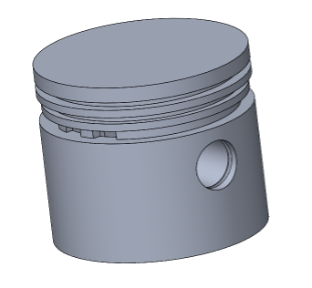
\includegraphics[scale=0.8]{Immagini/PistoneCAD.png}
    \caption{Modello CAD SOLIDWORKS del pistone}
    \label{fig:PistoneCAD}
\end{figure}
\begin{figure}[h]
    \centering
    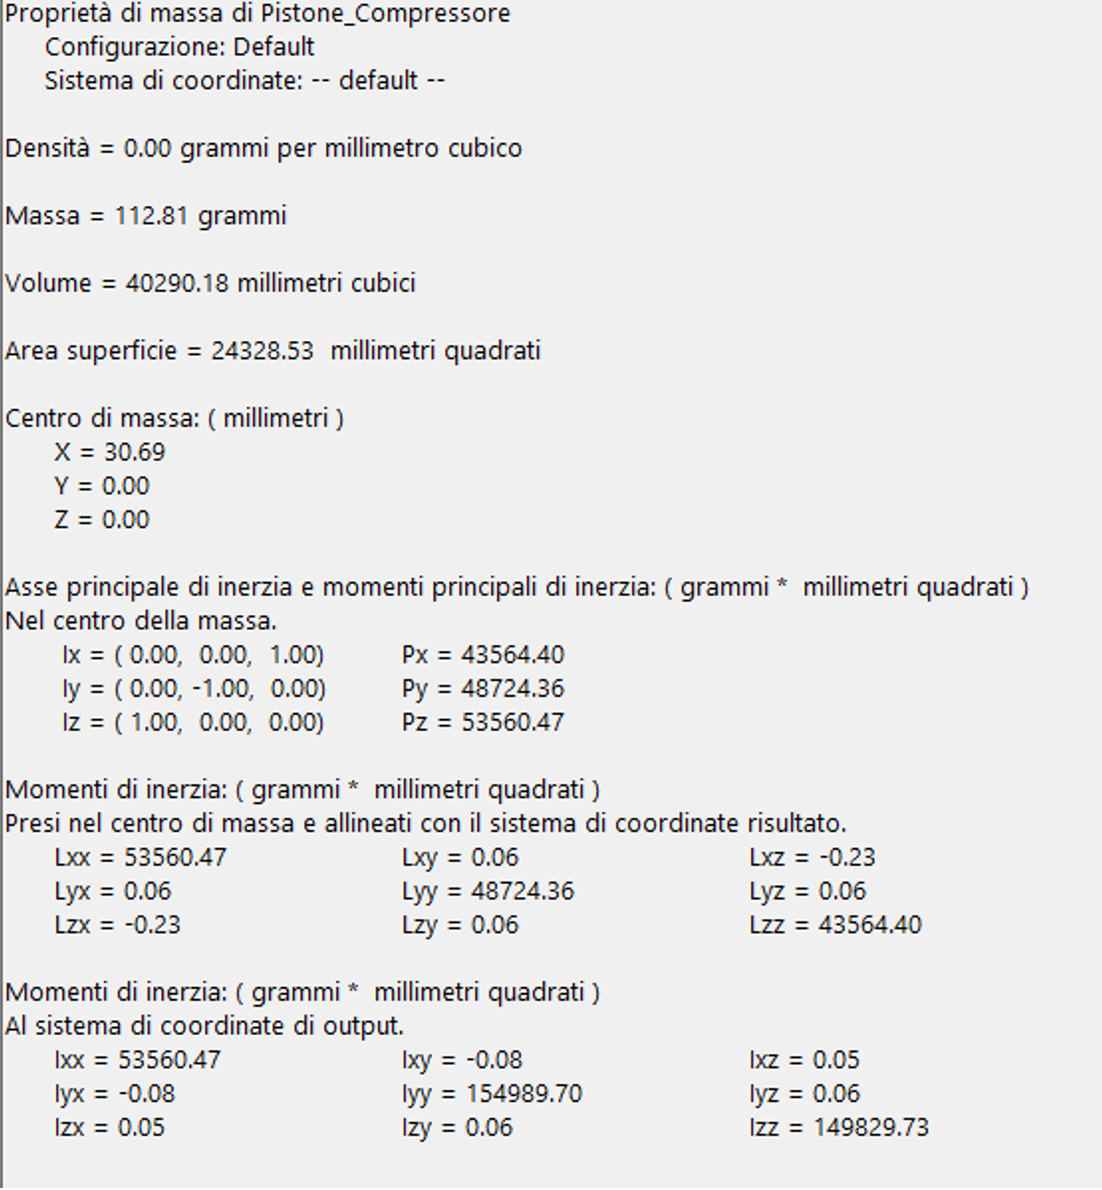
\includegraphics[scale=0.47]{Immagini/CaratteristichePistone.png}
    \caption{Caratteristiche pistone ricavate mediante sofrtware SOLIDWORKS}
    \label{fig:Pistone}
\end{figure}
\newpage
\subsubsection{Biella}
\begin{figure}[h]
\centering
   {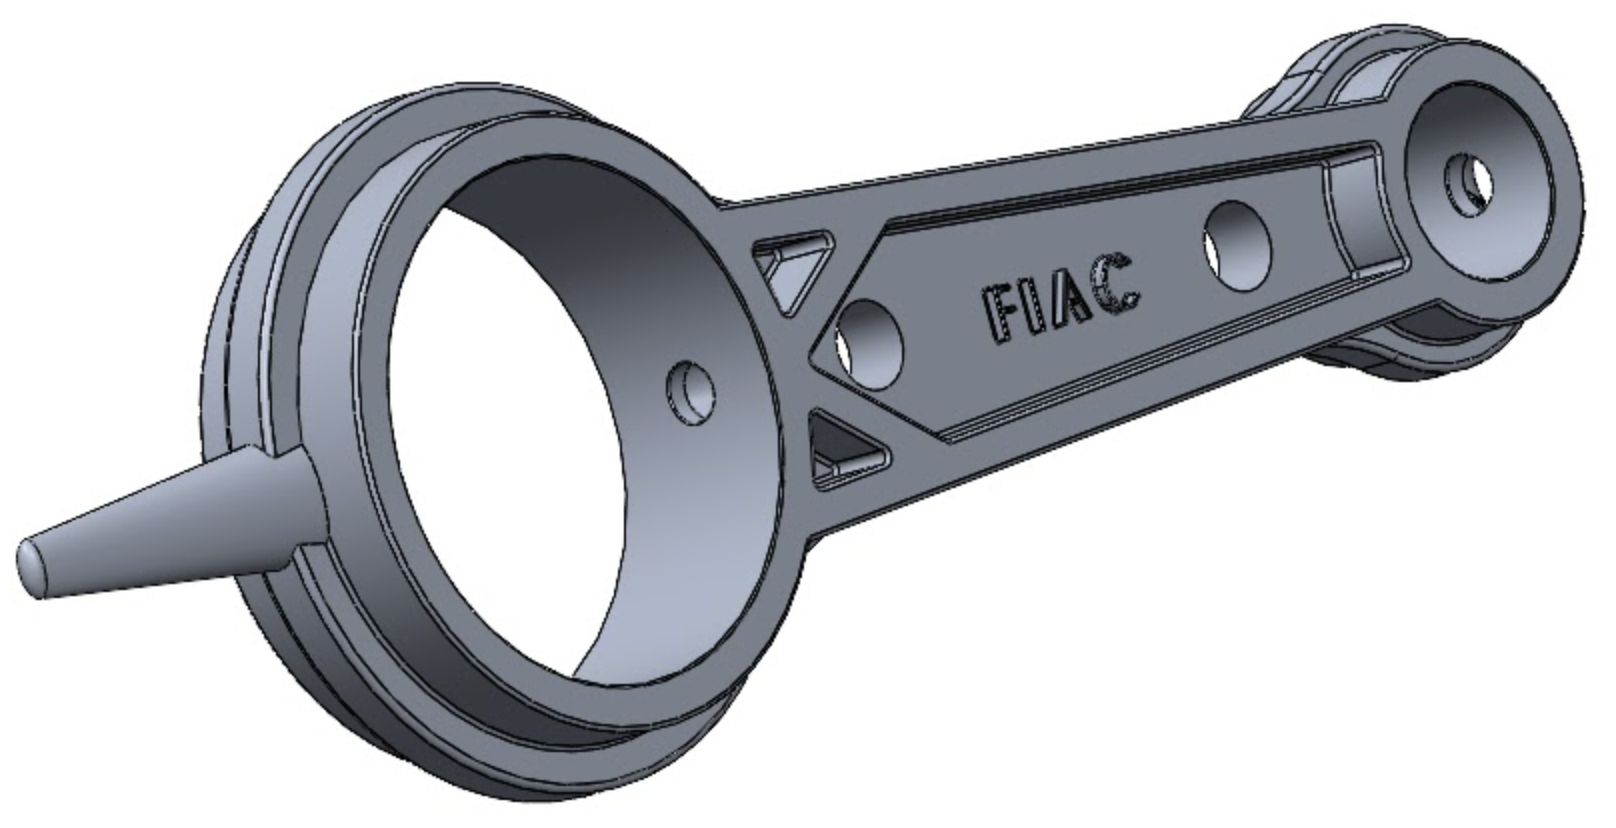
\includegraphics[width=.46\textwidth]{Immagini/Biella1.png}} \quad
   {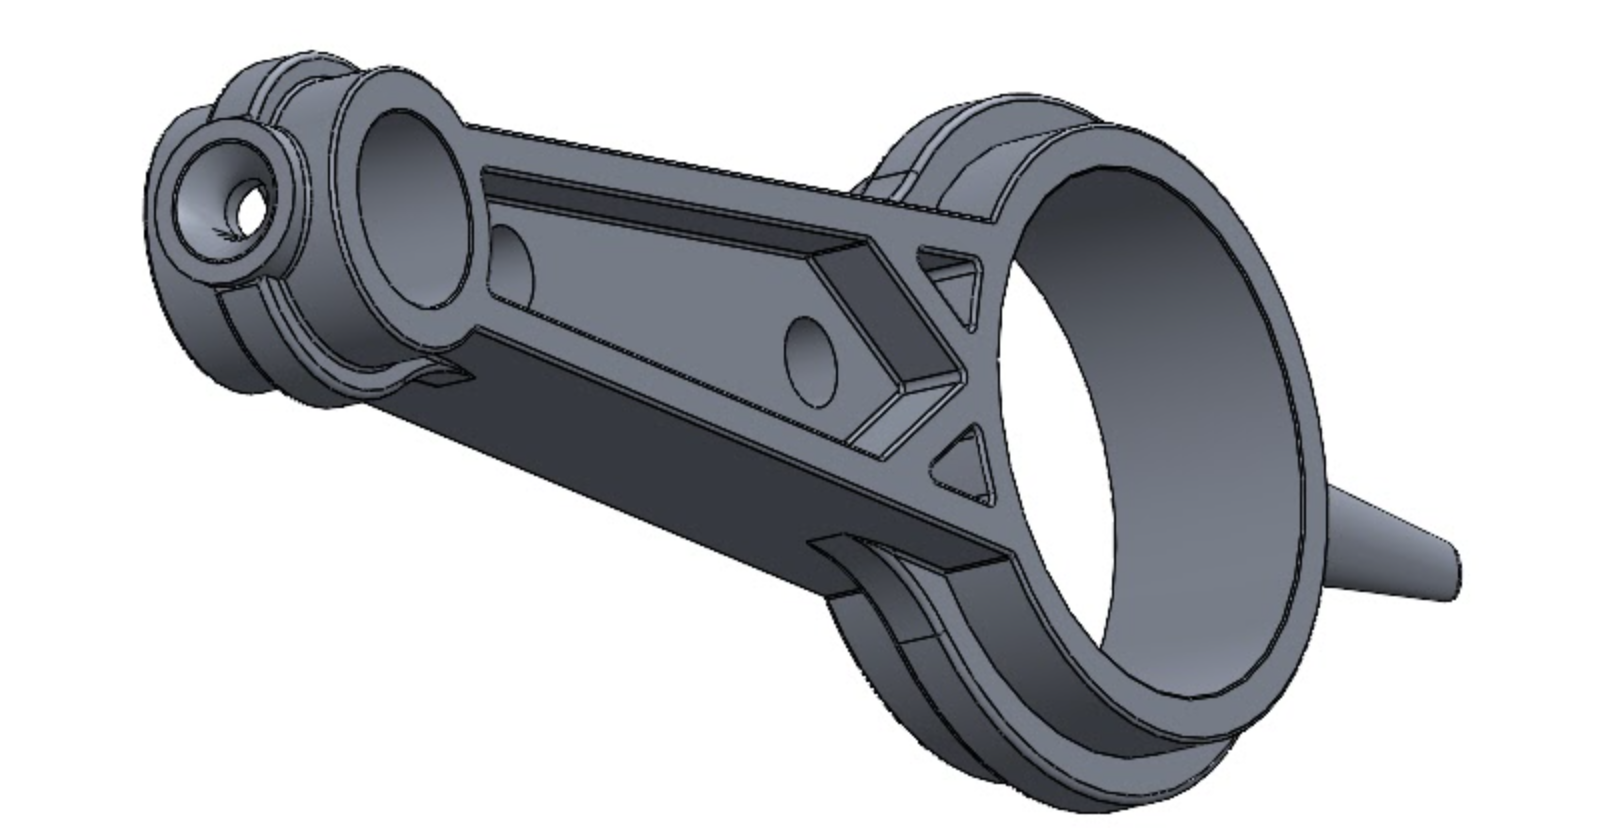
\includegraphics[width=.49\textwidth]{Immagini/Biella2.png}}
\caption{Modello CAD SOLIDWORKS della biella}
\label{fig:Biella}
\end{figure}
\begin{figure}[h]
    \centering
    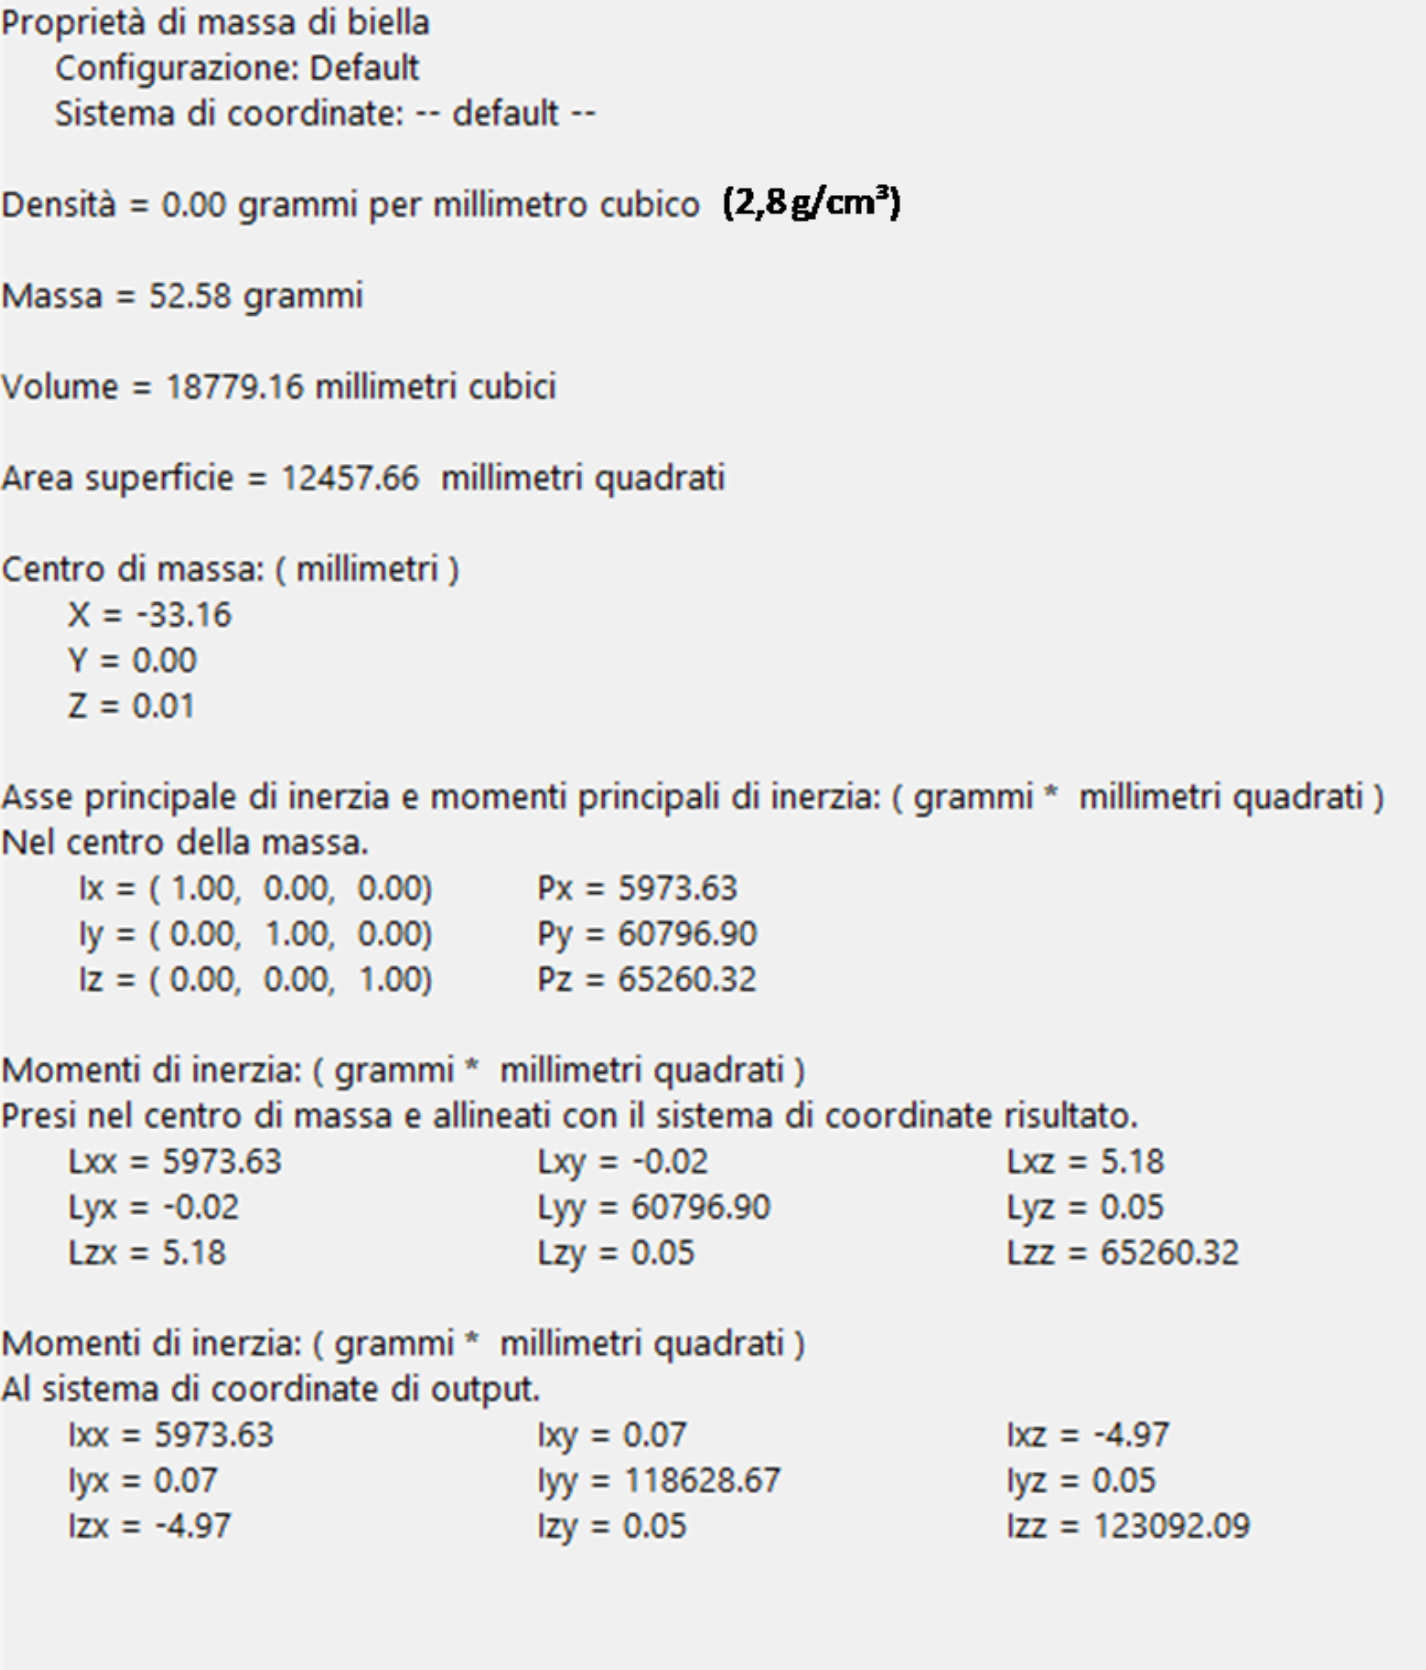
\includegraphics[scale=0.4]{Immagini/CaratteristicheBiella.png}
    \caption{Caratterstiche biella ricavate mediante software SOLIDWORKS}
    \label{fig:CaratteristicheBiella}
\end{figure}
\newpage
\subsubsection{Spinotto}
\begin{figure}[h]
\centering
   {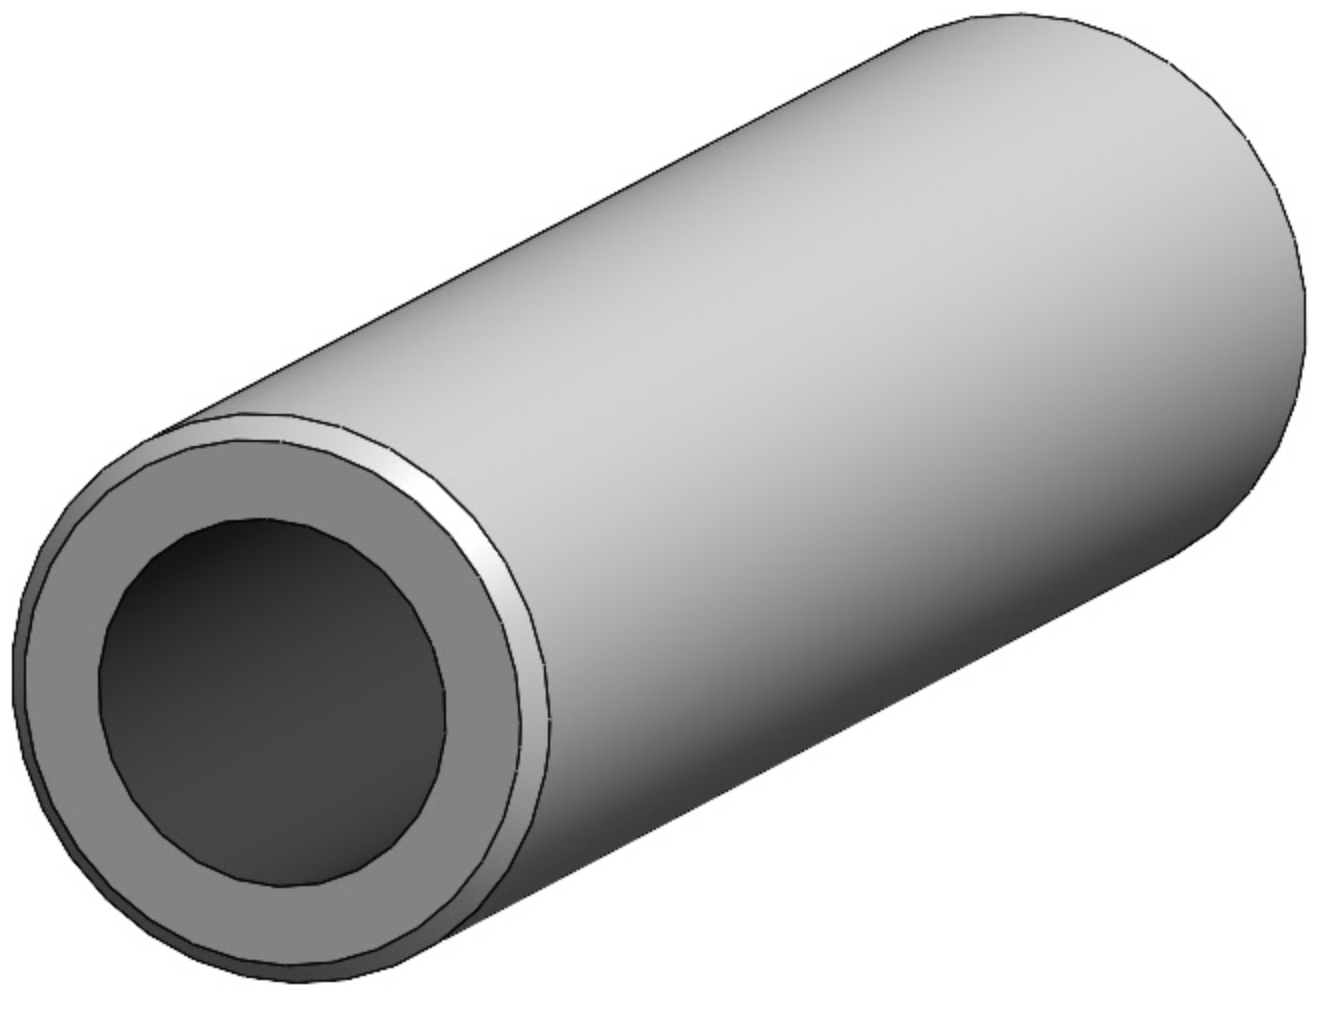
\includegraphics[width=.35\textwidth]{Immagini/Spinotto1.png}} \quad
   {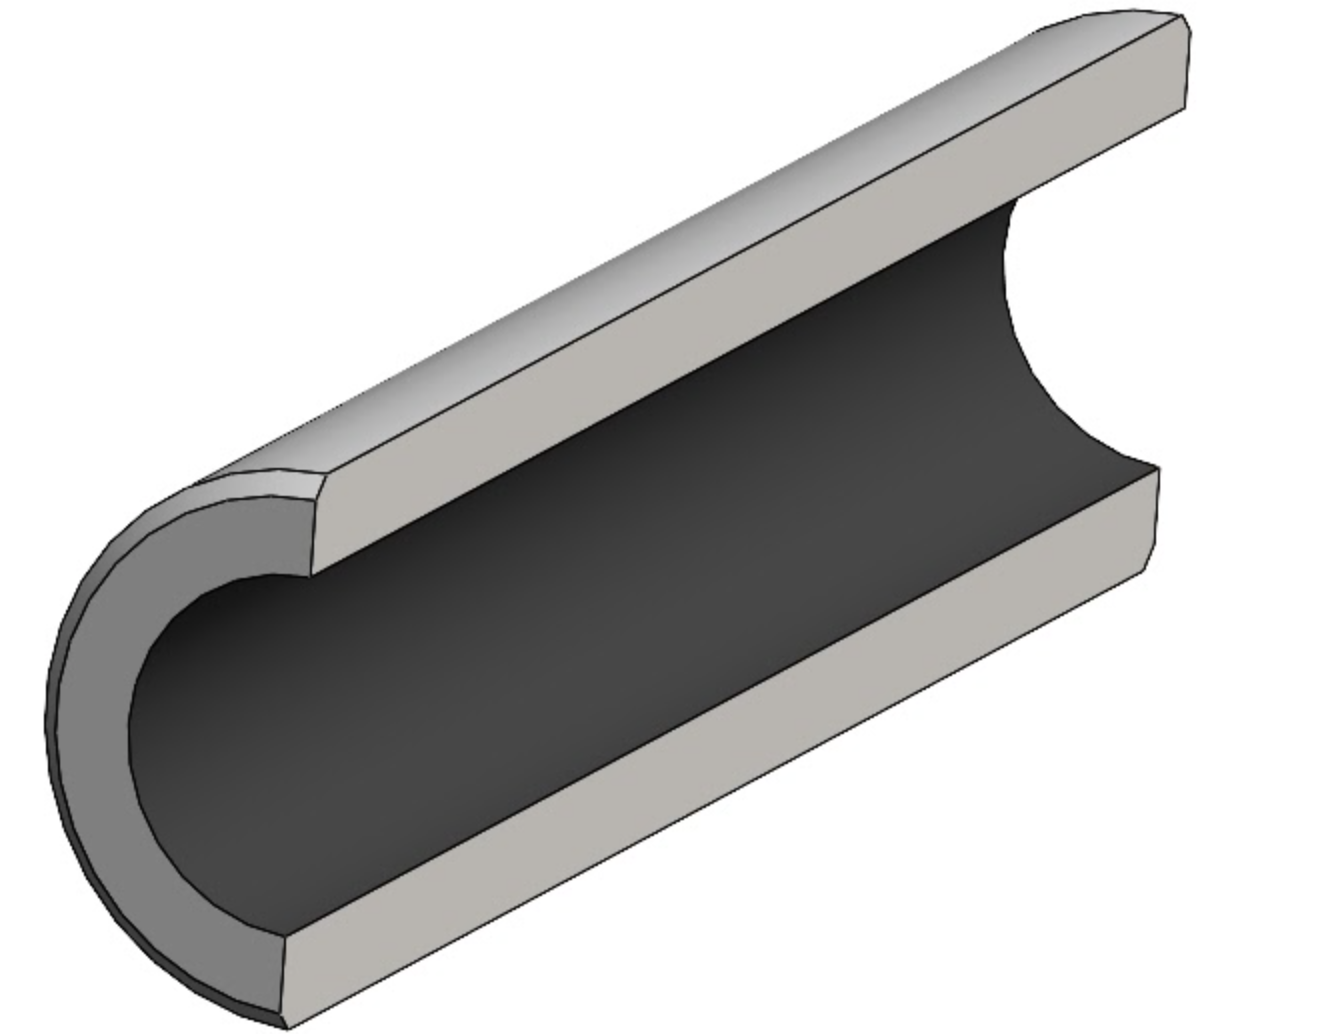
\includegraphics[width=.35\textwidth]{Immagini/Spinotto2.png}}
\caption{Modello CAD SOLIDWORKS dello spinotto}
\label{fig:Spinotto}
\end{figure}
\begin{figure}[h]
    \centering
    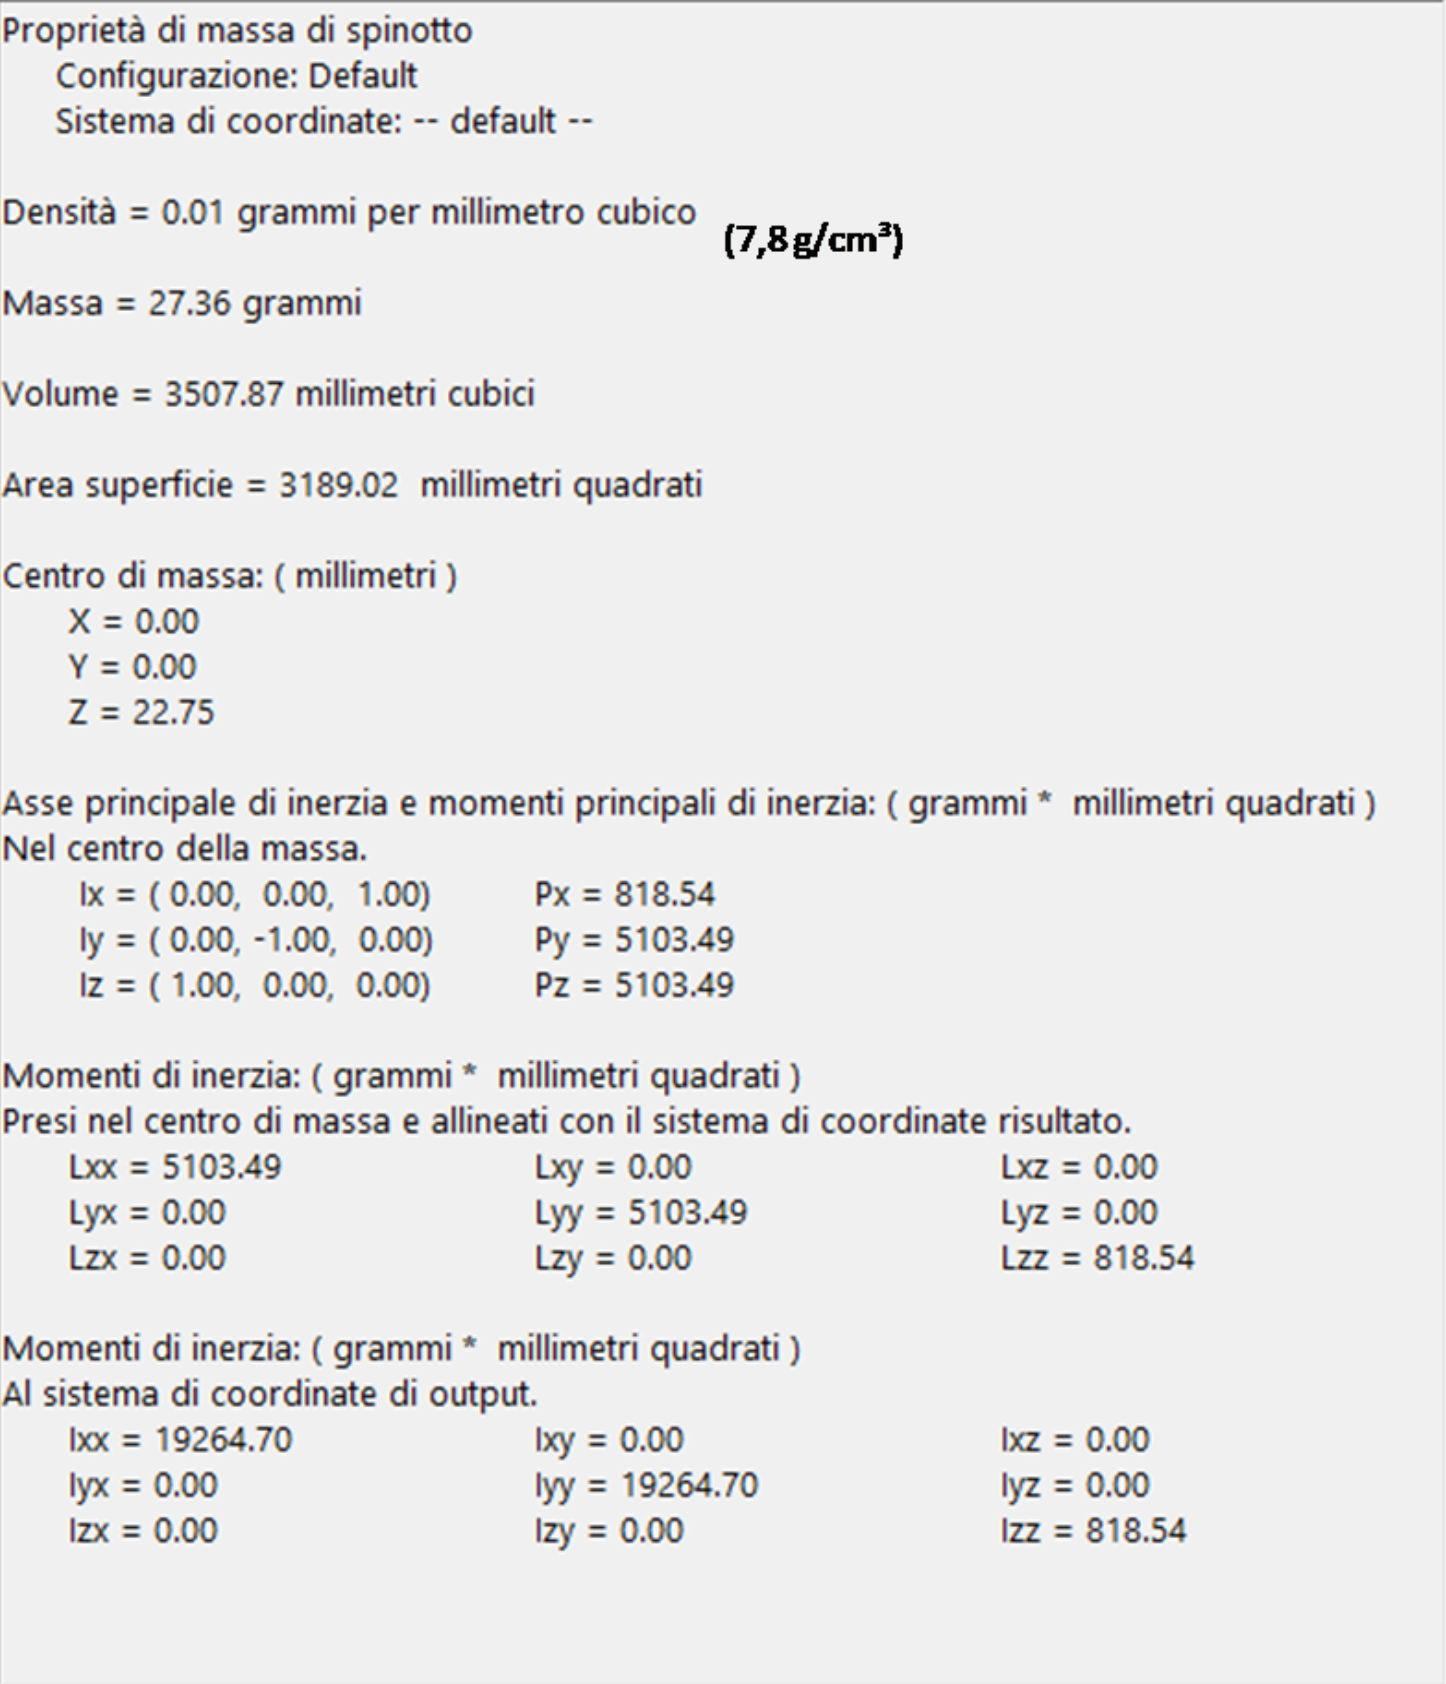
\includegraphics[scale=0.37]{Immagini/CaratteristicheSpinotto.png}
    \caption{Caratteristiche dello spinotto ricavate mediante software SOLIDWORKS}
    \label{fig:CaratteristicheSpinotto}
\end{figure}
\newpage
\subsubsection{Albero a gomiti}
\begin{figure}[h]
\centering
   {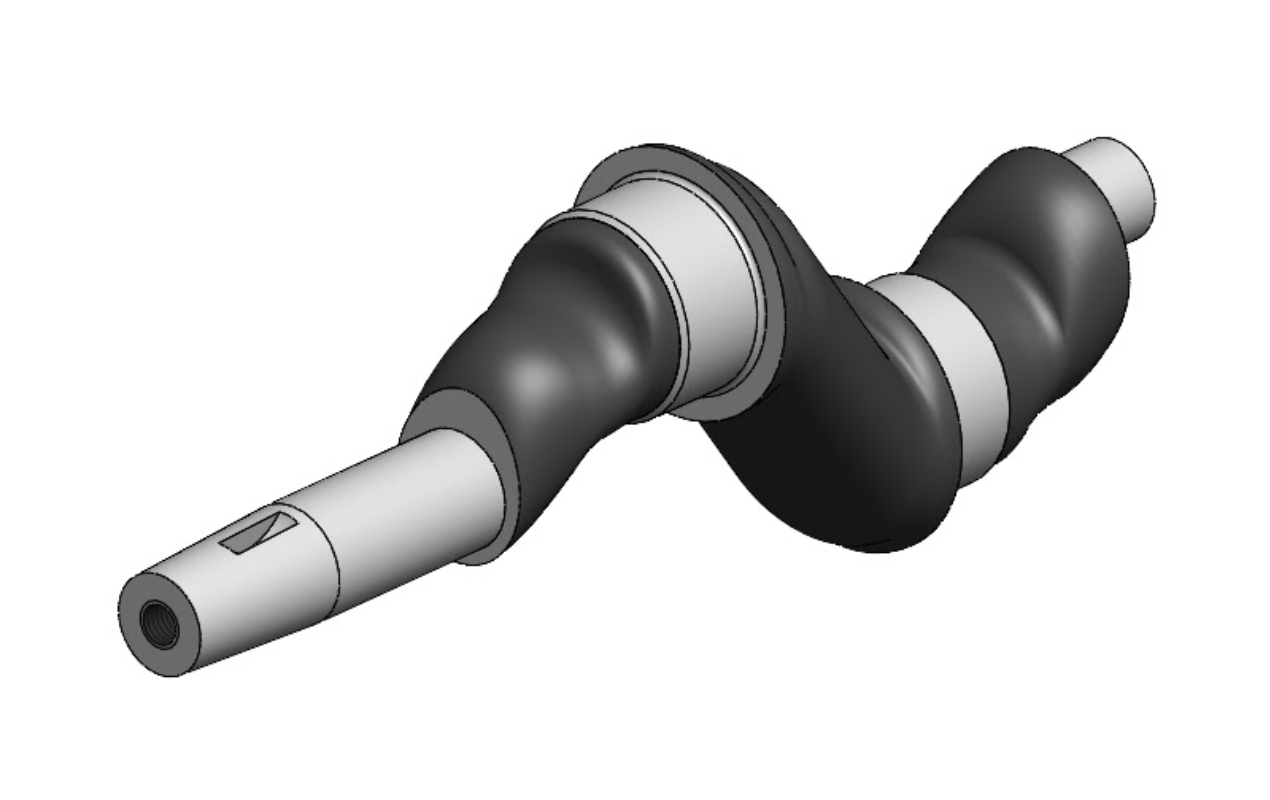
\includegraphics[width=.48\textwidth]{Immagini/Albero1.png}} \quad
   {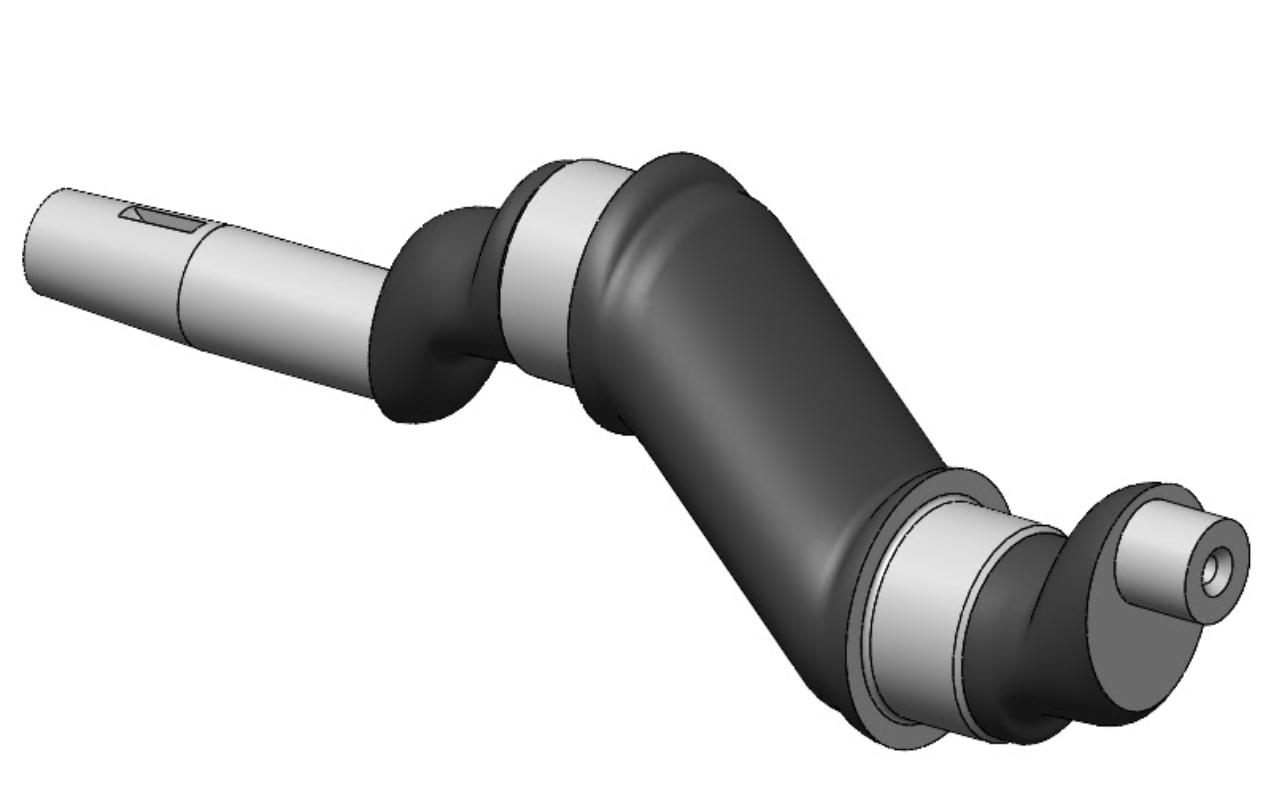
\includegraphics[width=.48\textwidth]{Immagini/Albero2.png}}
\caption{Modello CAD SOLIDWORKS dell'albero}
\label{fig:Albero}
\end{figure}
\begin{figure}[h]
    \centering
    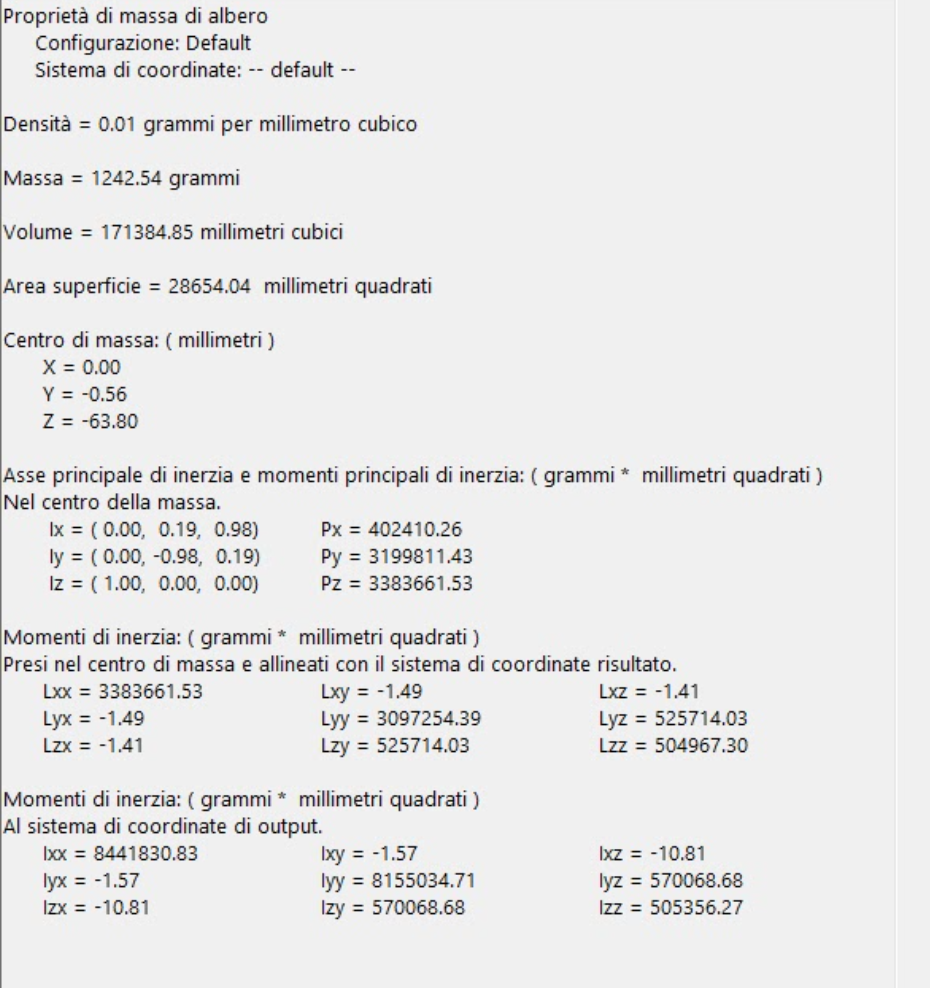
\includegraphics[scale=0.66]{Immagini/CaratteristicheAlbero.png}
    \caption{Caratteristiche dell'albero ricavate mediante software SOLIDWORKS}
    \label{fig:CaratteristicheAlbero}
\end{figure}
\newpage
\subsection{Andamento delle forze agenti in funzione dell'angolo di manovella}
Si analizzano ora le forze agenti sui vari elementi del cinematismo biella, pistone, spinotto e albero motore dovute all’effetto della pressione e alle azioni inerziali. 
\subsubsection{Pistone}
La forza complessiva che agisce sul pistone è data dalla somma del contributo dovuto alla pressione del fluido e quello dovuto all’inerzia dei corpi.
\paragraph{Forza dovuta alla pressione del fluido}
In questo caso il riferimento all’interno del quale la forza è stata calcolata è relativo, perché la sollecitazione è quella che agisce sul pistone; quindi, il punto di vista è all’interno del cilindro.\\
Per questo motivo la pressione istante per istante viene diminuita della pressione atmosferica. 
\begin{figure}[h]
    \centering
    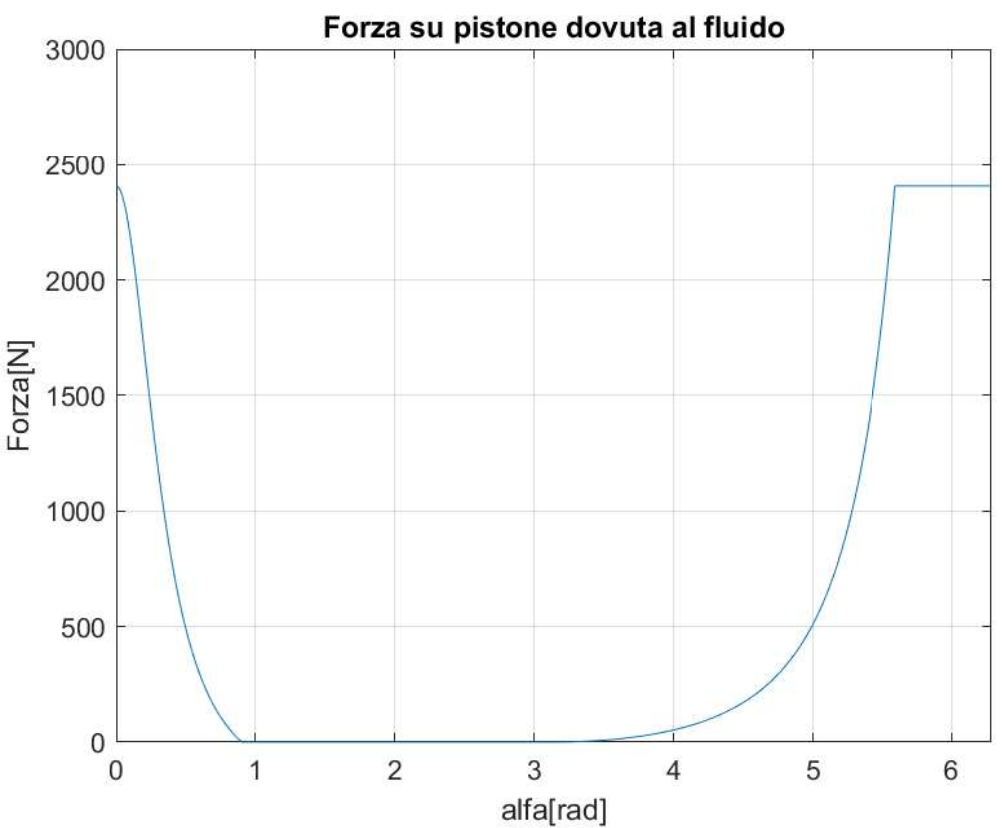
\includegraphics[scale=0.6]{Immagini/ForzaFluidoPistone.png}
    \caption{Forza esercitata dalla pressione del fluido sul pistone in funzione di $\alpha$}
    \label{fig:ForzaFluidoPistone}
\end{figure}
\begin{lstlisting}[frame=trBL]
%Calcolo forza su pistone%

Pressione=[ pressioneesp ya pressionecomp ym];  %raccolgo tutti i 
                                               %valori delle pressioni 
                                                %al variare degli 
                                                %angoli, per poi 
                                                %sottrarci 101325 Pa
alfatot=[ alfaesp xa alfacomp xm ]; %vettore degli angoli
Prel=Pressione-101325;
Forzapistone1= Apist*Prel; %1 perche dovuta al fluido
plot(alfatot,Forzapistone1);
xlabel('alfa[rad]'),ylabel('Forza[N]'),
      title('Forza su pistone dovuta al fluido'),
      grid on,xlim([0 2*pi]),ylim([0 3000]);
\end{lstlisting}
\paragraph{Forza dovuta all'inerzia del pistone}Per ricavare la forza dovuta all’inerzia è necessario ricavare l’accelerazione del pistone in funzione dell’angolo di manovella.\\
\\
Derivando due volte la formula dello spostamento in funzione del tempo (eq.(\ref{spostamento})) è possibile ricavare l’accelerazione cercata:
\begin{equation}
    a=\frac{dv}{dt}=\frac{d^2s}{{dt}^2}=\omega^2r(cos(\alpha)+\frac{cos(2\alpha)}{\lambda})
\end{equation}
con $\omega=\frac{2\pi n}{60}$.
\\
L'andamento dell'accelerazione in funzione dell'angolo di manovella è stato ricavato in ambiente Matlab.
\begin{figure}[h]
    \centering
    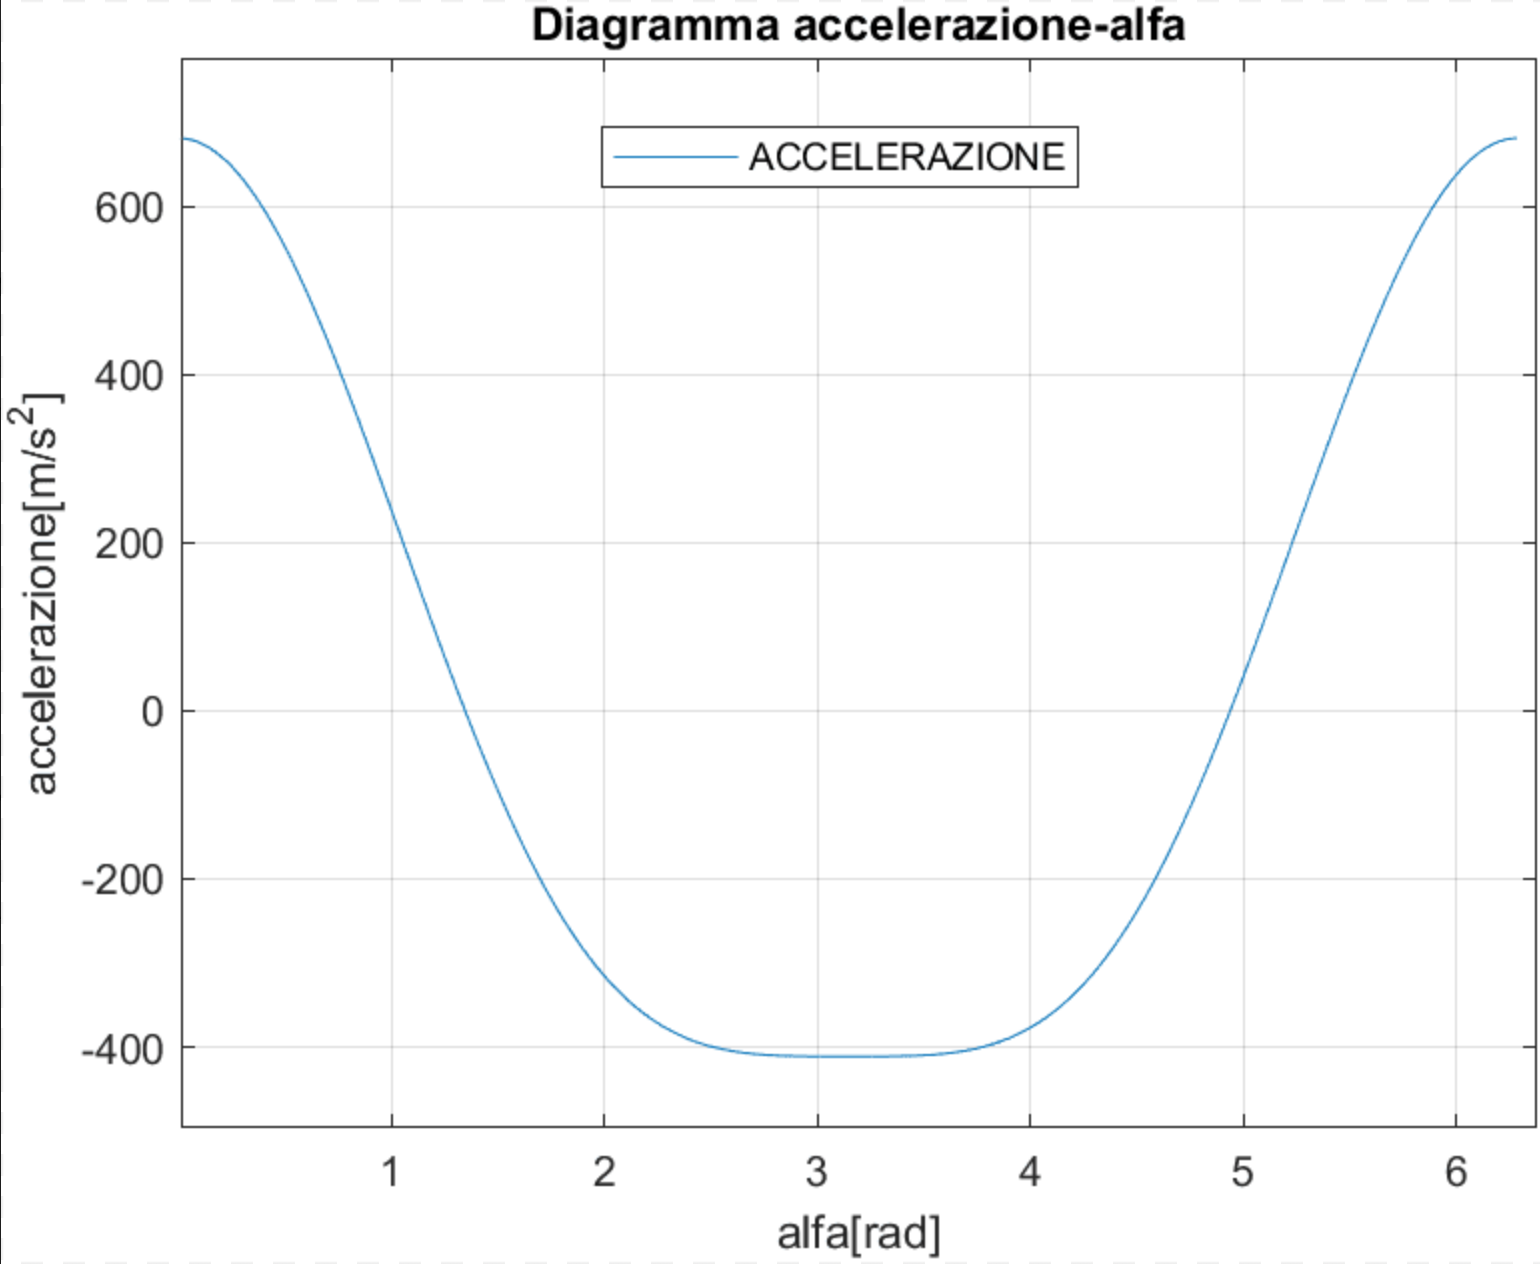
\includegraphics[scale=0.35]{Immagini/GraficoAccelerazionePistone.png}
    \caption{Accelerazione pistone in funzione dell'angolo di manovella}
    \label{fig:GraficoAccelerazionePistone}
\end{figure}
\begin{lstlisting}[frame=trBL]
%Grafico accelerazione al variare di alfa

alfa=linspace(0,2*pi,2000)
accelerazione=(w^2)*r*((cos(alfa))+(cos(2*alfa)*lambda^(-1)));
plot(alfa,accelerazione);
xlabel('alfa[rad]'),ylabel('accelerazione[m/s^2]'),
      title('Diagramma accelerazione-alfa'),grid on;xlim(0,2*pi);
\end{lstlisting}
\newpage
La forza di inerzia si definisce come:
\begin{equation}
    F_i=-m_{pistone}\cdot a_{pistone}
\end{equation}
Questa forza ha una direzione parallela a quella del moto del pistone e con verso discorde a quello dell’accelerazione.\\
La massa del pistone è stata determinata precedentemente mediante software di modellazione SOLIDWORKS ($m_p$=112,81 g).\\
Anche in questo caso è stato ricavato l'andamento mediante uno script Matlab dell'andamento di questa forza in funzione dell'angolo di manovella.
\begin{figure}[h]
    \centering
    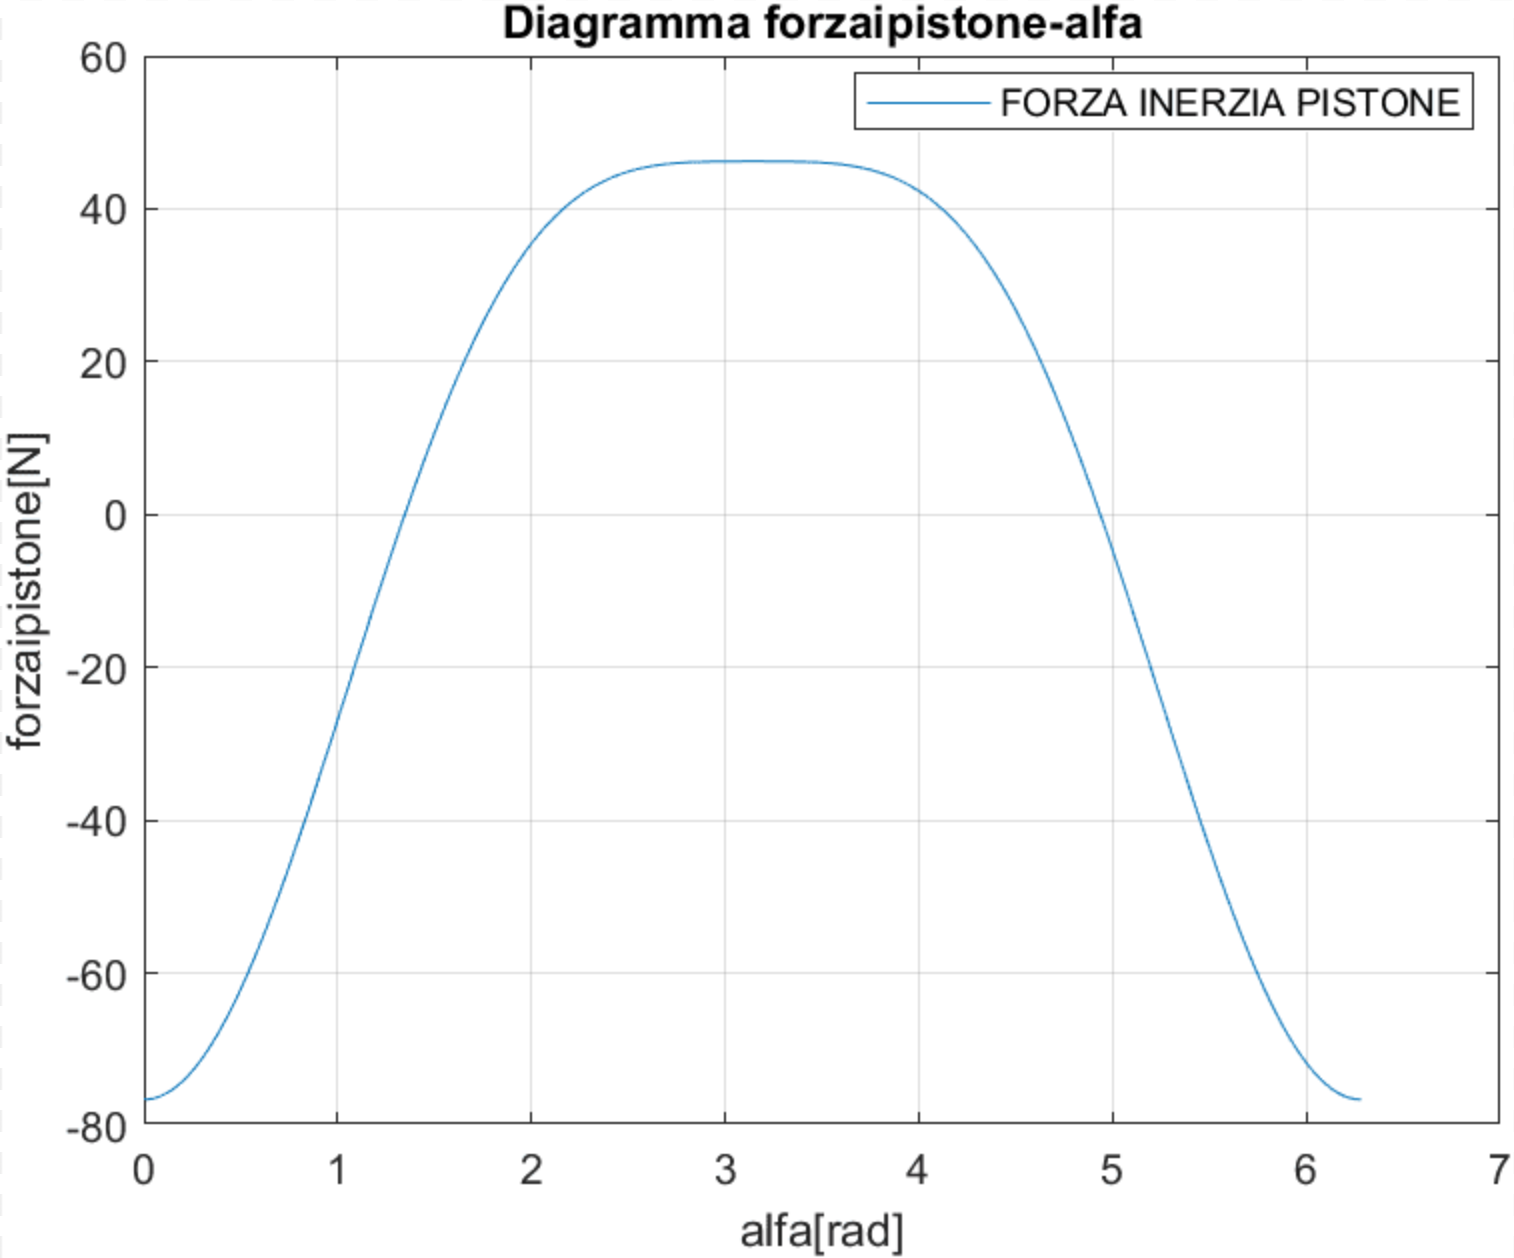
\includegraphics[scale=0.33]{Immagini/GraficoInerziaPistone.png}
    \caption{Forza dovuta all'inerzia del pistone al variare di $\alpha$}
    \label{fig:GraficoInerziaPistone}
\end{figure}
\begin{lstlisting}[frame=trBL]
%Grafico forza inerzia al variare di alfa

mp=0.11238 %massa pistone [Kg]
forzaipistone=-mp*accelerazione;
plot(alfa,forzaipistone);

xlabel('alfa[rad]'),ylabel('forzaipistone[N]'),
      title('Diagramma forzaipistone-alfa'),
      grid on;xlim(0,2*pi);
\end{lstlisting}
\paragraph{Forza dovuta all'inerzia della biella} Per studiare le sollecitazioni agenti sul pistone dovute alla biella è necessario fare una semplificazione. Si passa dallo studio di un corpo rigido tridimensionale avente massa e tensore di inerzia fissati, all’analisi di un sistema equivalente costituito da due masse puntiformi concentrate alle estremità.\\
Per poter adoperare questo stratagemma, bisogna imporre che l’energia cinetica rimanga invariata, così come il baricentro.\\
Condizioni per le quali le precedenti assunzioni sono verificate: 
\begin{equation}
    m_A+m_B=m
\end{equation}
\begin{equation}
    m_Aa^2+m_Bb^2+J_0=J
\end{equation}
\begin{equation}
    m_Aa=m_Bb
\end{equation}
\begin{figure}[h]
\centering
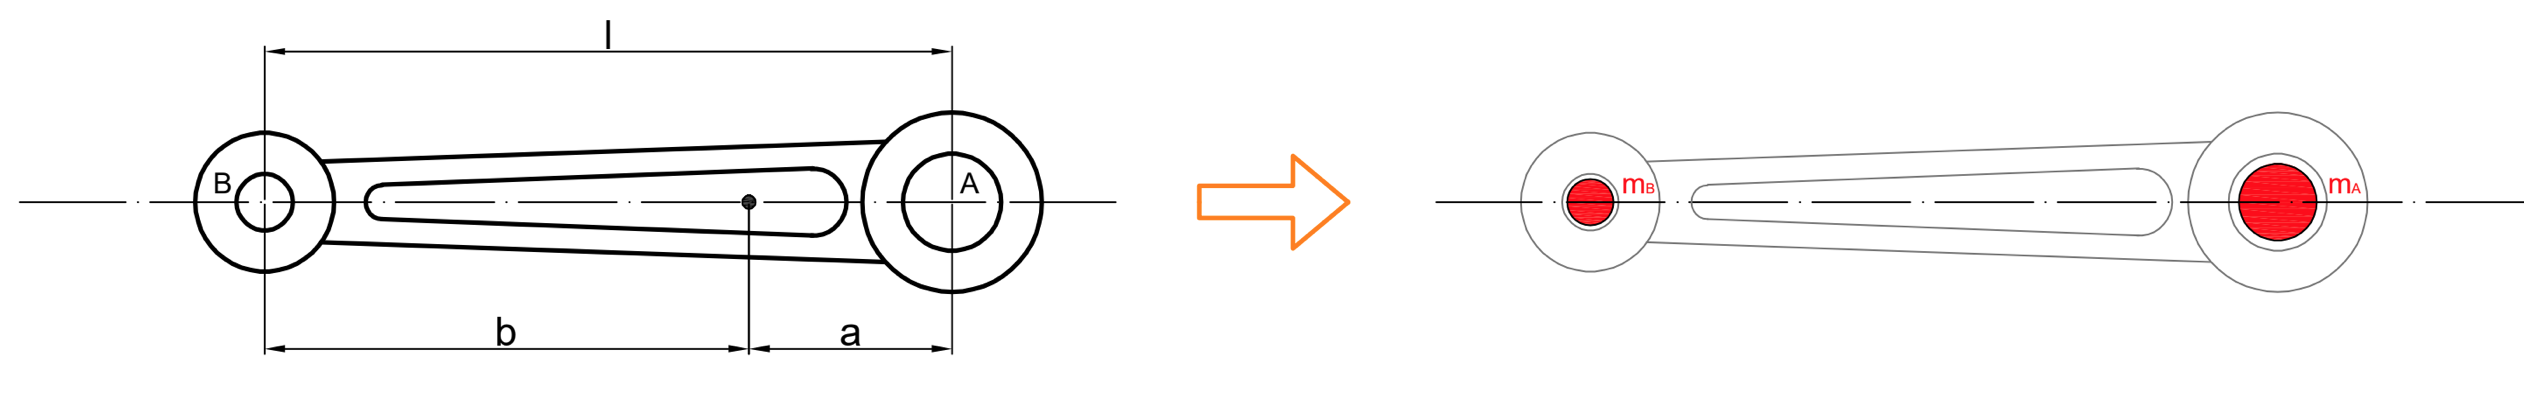
\includegraphics[scale=0.3]{Immagini/SostituzioneBiella.png}
\caption{Semplificazione per lo studio della biella}
\label{fig:SostituzioneBiella}
\end{figure}
\\
I termini $m_A$ e $m_B$ sono le due masse, $J_0$ è il momento d'inerzia puro, m è la massa della biella e $J$ è il suo momento di inerzia rispetto a un asse baricentrico ortogonale al piano del moto. \\
Il termine $J_0$ è un termine fittizio che è necessario introdurre come artificio algebrico (talvolta trascurabile) per steli snelli e che quasi sempre corrisponde ad una correzione di segno negativo. \\
Le distanze a e b sono prese in valore assoluto dal baricentro G ai punti A e B nei quali sono collocate $m_A$ e $m_B$.\\
Dalle condizioni scritte precedentemente si ottiene: 
\begin{equation}
    m_A=\frac{mb}{l}
\end{equation}
\begin{equation}
    m_B=\frac{ma}{l}
\end{equation}
\begin{equation}
    J_0=J-mab
\end{equation}
Dall’analisi delle proprietà di massa della biella su SOLIDWORKS (Fig.\ref{fig:CaratteristicheBiella}) è stato possibile ricavare la posizione del baricentro, quindi le distanze a e b e il momento d’inerzia J. 
\begin{equation}
    J\left(P_z\right)=6,5311{\cdot10}^{-5}\ kgm^2
\end{equation}
\begin{equation}
    a=33.16{\cdot10}^{-3}\ m
\end{equation}
\begin{equation}
    b=l-a=\left(85-33,16\right){\cdot10}^{-3}m=51,84{\cdot10}^{-3}\ m.
\end{equation}
Noti questi parametri, si ricavano dalle formule prima citate le grandezze associate allo studio della biella: 
\begin{equation}
    m_B=0,0205\ kg
\end{equation}
\begin{equation}
    m_A=m-m_B=\left(52,61{\cdot10}^{-3}-0,0205\right)\ kg=0,03209\ kg
\end{equation}
\begin{equation}
    J_0=-2,5126{\cdot10}^{-5}\ kgm^2.
\end{equation}
Avendo supposto di avere parte della massa di biella concentrata sul piede, essa durante il moto sarà soggetta a un’accelerazione che si tradurrà in una forza d’inerzia trasmessa al pistone.\\
La forza d’inerzia sarà: 
\begin{equation}
    F_i=-m_B\cdot a_{\mbox{pistone}}
\end{equation}
il cui andamento è stato ricavato mediante uno script Matlab.
\begin{figure}[h]
    \centering
    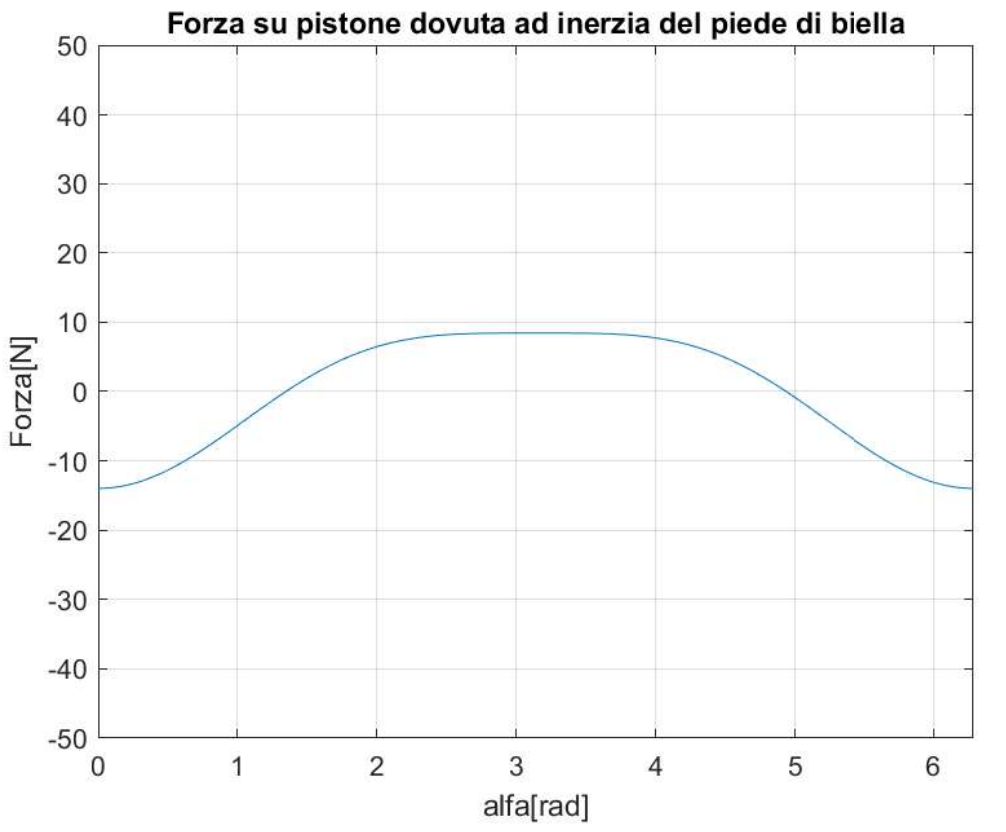
\includegraphics[scale=0.6]{Immagini/GraficoInerziaPiede.png}
    \caption{Andamento della forza di inerzia dovuta al piede di biella}
    \label{fig:GraficoInerziaPiede}
\end{figure}
\begin{lstlisting}[frame=trBL]
%Grafico forze di inerzia dovute alla massa del piede di biella

mbiella=52.61*(10^-3); %[kg]
b=33.16*(10^-3); %distanza tra centro di massa e testa di biella [m]
a=51.84*(10^-3); %distanza tra centro di massa e piede di biella[m]
l=85*(10^-3); %interasse tra testa e piede di biella [m]
mB=(mbiella*b)*(l^-1);
Forzapistone3=-mB*accelerazione;
plot(alfa,Forzapistone3);
xlabel('alfa[rad]'),ylabel('Forza[N]'),
      title('Forza su pistone dovuta ad inerzia de piede di biella'),
      grid on,xlim([0 2*pi]),ylim([-50 50]);
\end{lstlisting}
\paragraph{Forza dovuta all'inerzia dello spinotto} Essendo lo spinotto solidale al pistone durante il moto, anch’esso contribuirà a geneare una componente d’inerzia sul pistone. \\
Tale forza può essere quantificata come: 
\begin{equation}
    F_i=-m_{\mbox{spinotto}}\cdot a_{\mbox{pistone}}
\end{equation}
il cui andamento è ricavato mediante uno script Matlab.
\newpage
\begin{figure}[h]
    \centering
    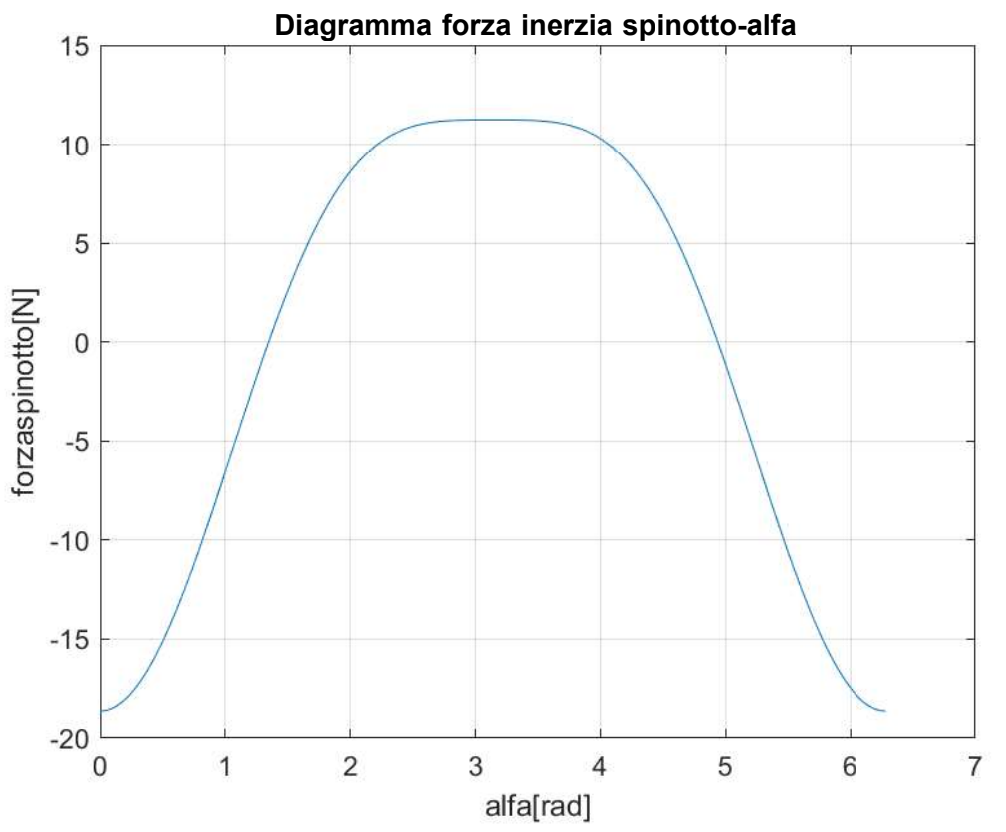
\includegraphics[scale=0.5]{Immagini/GraficoInerziaSpinotto.png}
    \caption{Andamento della forza di inerzia dovuta allo spinotto}
    \label{fig:GraficoInerziaSpinotto}
\end{figure}

\begin{lstlisting}[frame=trBL]
%Grafico forze di inerzia dovute alla massa dello spinotto

mspinotto=27.36*(10^-3); %[kg]
forzaspinotto=-mspinotto*accelerazione;
plot(alfa,forzaspinotto);
xlabel('alfa[rad]'),ylabel('forzaspinotto[N]'),
       title('Diagramma forza inerziaspinotto-alfa'),
       grid on;xlim(0,2*pi);
\end{lstlisting}
Di seguito si riportano in un unico grafico tutti i contributi di forze dovuti alla pressione e alle inerzie che agiscono sul pistone.\\
Si può notare come queste ultime siano trascurabili rispetto all’entità della forza generata dalla pressione del fluido.
\begin{figure}[h]
\centering
   {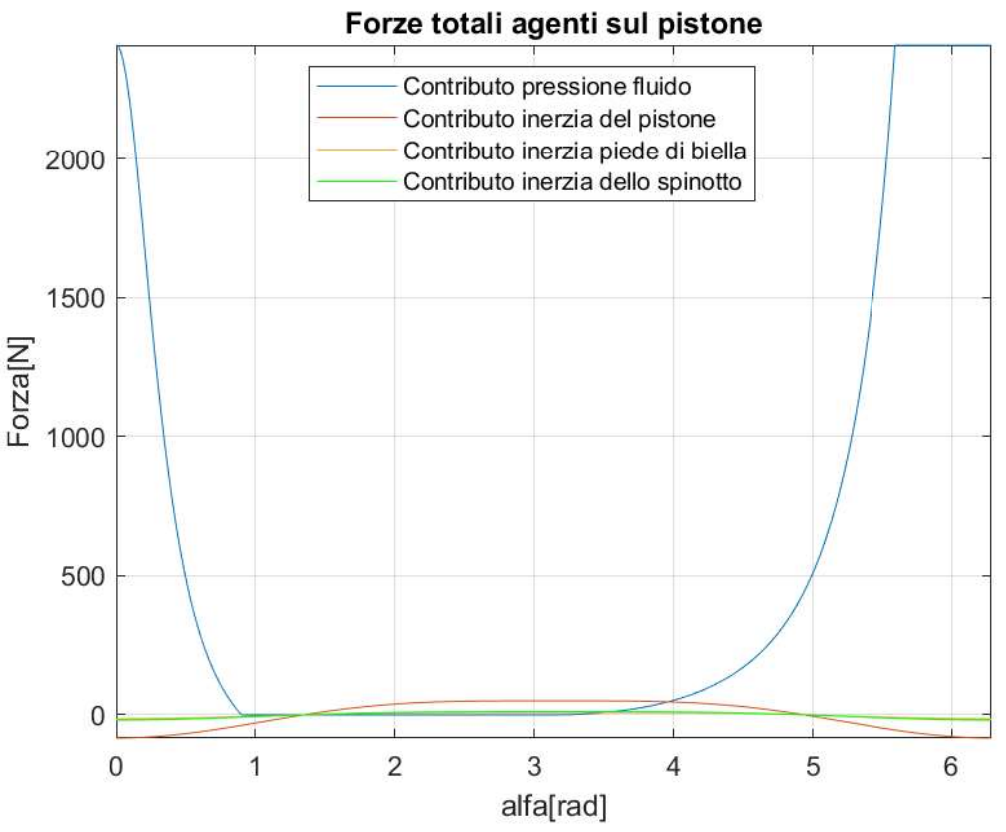
\includegraphics[width=.48\textwidth]{Immagini/GraficoInsiemeForze1.png}} \quad
   {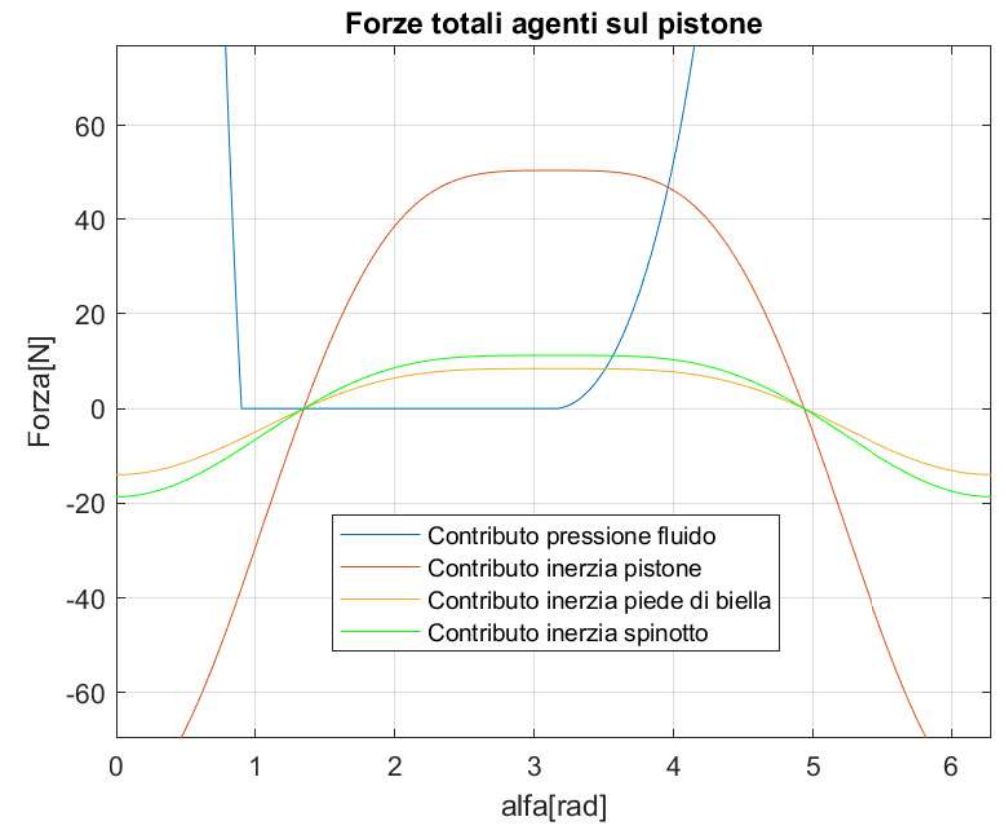
\includegraphics[width=.48\textwidth]{Immagini/GraficoInsiemeForze2.png}}
\caption{Insieme delle forze agenti sul pistone al variare di $\alpha$}
\label{fig:GraficoInsiemeForze}
\end{figure}
\newpage
\begin{lstlisting}[frame=trBL]
%Grafico insieme delle forze

plot(alfatot,Forzapistone1);
hold on     
plot(alfa,forzaipistone);
plot(alfa,Forzapistone3);
plot(alfa,forzaspinotto,'g');
xlabel('alfa[rad]'),ylabel('Forza[N]'),
       title('Forze totali agenti sul pistone'),
       grid on,xlim([0 2*pi]),ylim([-50 50]);
hold off
\end{lstlisting}
Sommando tutti i contributi delle forze agenti sul pistone la risultante avrà un andamento come mostrato in figura:
\begin{figure}[h]
    \centering
    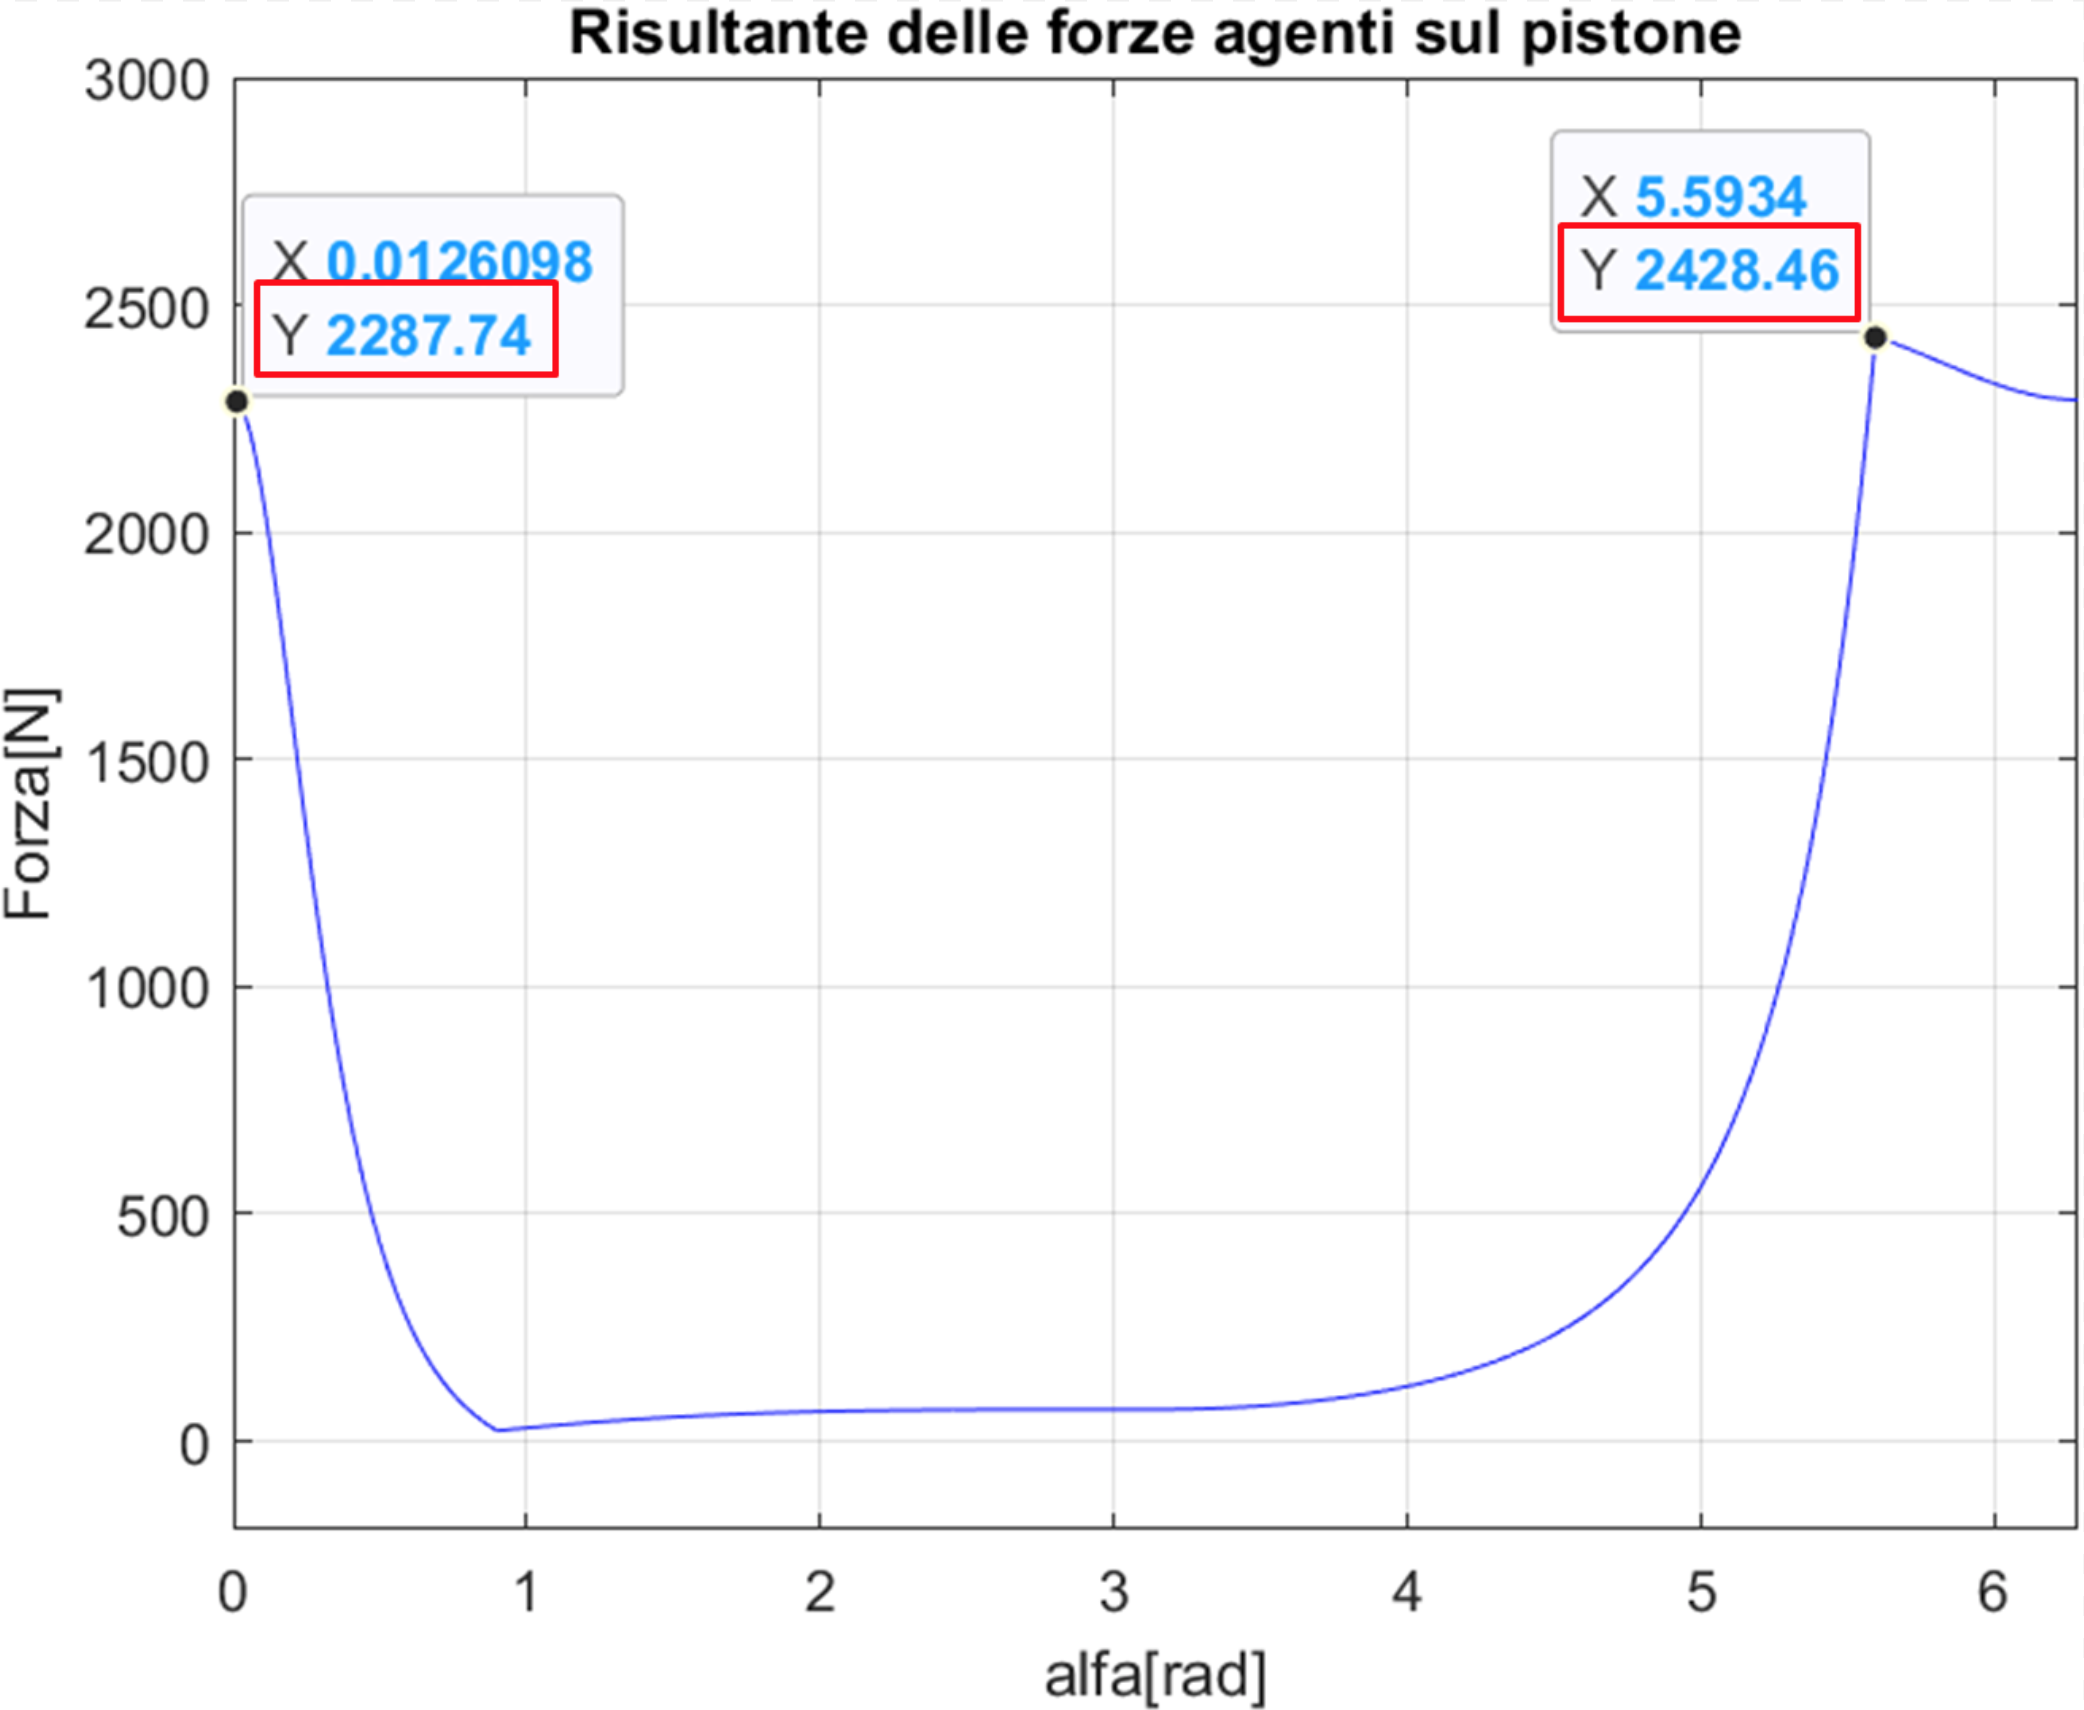
\includegraphics[scale=0.3]{Immagini/GraficoForzaRisultante.png}
    \caption{Andamento della forza risultante sul pistone al variare di $\alpha$}
    \label{fig:GraficoForzaRisultante}
\end{figure}
\begin{lstlisting}[frame=trBL]
%Grafico andamento forza totale

Ftot=forzaspinotto+Forzapistone3,+Forzapistone1+forzaipistone;
plot(alfa,Ftot)

xlabel('alfa[rad]'),ylabel('Forza[N]'),
      title('Risultante delle forze agenti sulpistone'),
      grid on,xlim([0 2*pi]),ylim([-100 3000]);
\end{lstlisting}
Come è possibile dedurre dal grafico, le posizioni in cui il pistone è soggetto a maggiori sollecitazioni comprendono dal punto di fine compressione a quello di inizio espansione.\\
La forza massima agente si può assumere da grafico pari a 2428.46 N.\\
Per i calcoli strutturali che verranno effettuati successivamente si ipotizzerà di avere una forza massima agente sul pistone pari a $F_{\mbox{pistone}} = 2500\ N$, contemplando già da qui un fattore di sicurezza per considerare eventuali valutazioni approssimative effettuate durante l’analisi dei carichi del cinematismo (per esempio la considerazione del ciclo ideale per i calcoli, il fatto che la modellazione CAD non è perfettamente fedele alla realtà e la scelta del materiale). 
\subsubsection{Spinotto}
Le forze che agiscono sullo spinotto sono le stesse che agiscono sul pistone e quindi quelle che possono essere osservate in Fig.\ref{fig:GraficoForzaRisultante}.\\
Quindi anche in questo caso per i calcoli strutturali, esattamente come quanto detto per il pistone, considereremo una forza massima agente pari a $F_{\mbox{spinotto}} = 2500\ N$. 
\subsubsection{Biella}
Le forze che agiscono sulla biella sono:
\paragraph{Forza agente sul piede di biella}La forza totale agente sul piede di biella è quella trovata precedentemente dovuta a pressione del fluido, inerzie di pistone, spinotto e piede di biella. \\
L’andamento in funzione dell’angolo di manovella è quindi analogo a quello osservato per il pistone (Fig.\ref{fig:GraficoForzaRisultante}).  La sollecitazione sulla biella si divide in due componenti, una parallela all’asse della biella (compressione) e una ortogonale (flessione). 
\paragraph{Forza di inerzia centrifuga sulla testa di biella}La forza di inerzia dovuta alla rotazione della testa di biella attorno all’asse dell’albero ha direzione radiale ed è indipendente, in modulo, dall’angolo di manovella $\alpha$.\\
Il modulo può essere quantificato con la seguente formula: 
\begin{equation}
    F_{c1}=m_Ar\omega^2
\end{equation}
con $m_A$ massa della testa di biella pari a 0,03209 kg, r raggio di manovella pari a 0,021 m e $\omega$ velocità angolare di rotazione pari a $\omega=\frac{2\pi n}{60}=161,27\ rad/s$.\\
Si ottiene quindi $F_{c1}=17,53\ N$.\\
\\
Bisogna tenere conto, inoltre, della forza rotante centrifuga dovuta al moto della manovella, secondo la formula 
\begin{equation}
    F_{c2}=m_mr_m\omega^2
\end{equation}
si ottiene quindi $F_{c2}=327,7\ N$.\\
\\
In conclusione, la forza risultante agente sulla testa di  biella corrisponde a:
\begin{equation}
    F_c=F_{c1}+F_{c2}=\left(17,53+327,7\right)\ N=345,2\ N
\end{equation}
\newpage
\begin{figure}[h]
    \centering
    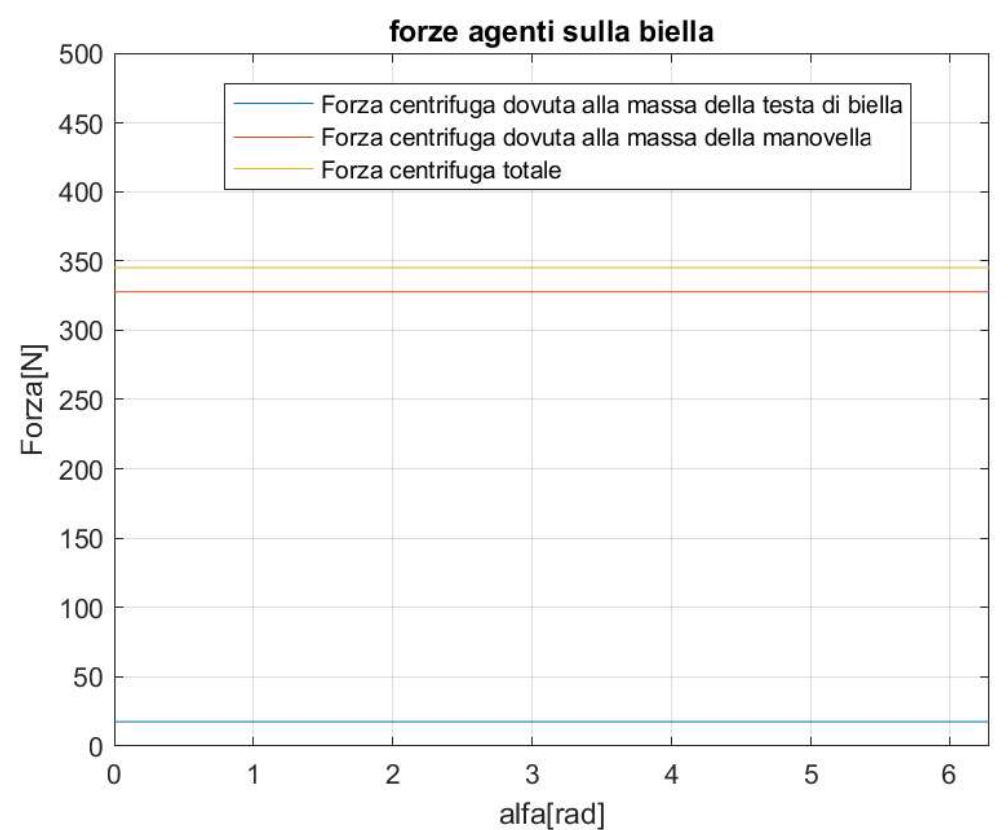
\includegraphics[scale=0.5]{Immagini/GraficoForzeCentrifugheBiella.png}
    \caption{Andamento forze centrifughe agenti sulla biella}
    \label{fig:GraficoForzeCentrifugheBiella}
\end{figure}
\begin{lstlisting}[frame=trBL]
%Calcolo forze su biella

%Dati
mB=0.03209; %massa B sistema equivalente biella [kg]
massaman=0.6; %massa di meta albero, ovvero della manovella [kg]
r=0.021; %raggio dimanovella [m]
n=1540; %velocita rotazione [giri/s]
l=0.085;
lambda=l*(r^-1); %[kg m^2]
Jo=-2.5126*(10^-5);

%Grandezze derivate
w=(2*pi*n)*(60^-1); %velocita angolare [rad/s]

%Forza centrifuga testa di biella
Fcent1=(mB)*r*w^2;
F=linspace(Fcent1,Fcent1,2000);
alfa=linspace(0,2*pi,2000);
plot(alfa, F);
xlabel('alfa[rad]'),ylabel('Forza[N]'),
      title('forze agenti sulla biella'),grid on,xlim([0 2*pi]);
      ylim([0 500]);
hold on
Fcent2=(massaman)*r*w^2;
F=linspace(Fcent2,Fcent2,2000);
alfa=linspace(0,2*pi,2000);
plot(alfa, F);
hold on
Ftot=Fcent1+Fcent2;
F=linspace(Ftot,Ftot,2000);
alfa=linspace(0,2*pi,2000);
plot(alfa, F);
hold off
\end{lstlisting}
\paragraph{Coppia di biella}
Ricordando la semplificazione ad uno schema equivalente adottato nello studio della biella è possibile stimare la coppia di inerzia rotante agente sul corpo.\\
La coppia di inerzia vale $-J_0\lambda\Omega^2\sin\alpha$.\\
Essa si può pensare come due forze di uguale intensità e direzione, ma di versi opposti, con la retta d’azione passante per A e per B e dirette perpendicolarmente all’asse di moto del pistone 
\begin{equation}
    F_{ci}=\left|\frac{J_0r}{l^2}\Omega^2sin{\left(\alpha\right)}\right|.
    \label{ForzaCoppiaBiella}
\end{equation}
\begin{figure}[h]
\centering
   {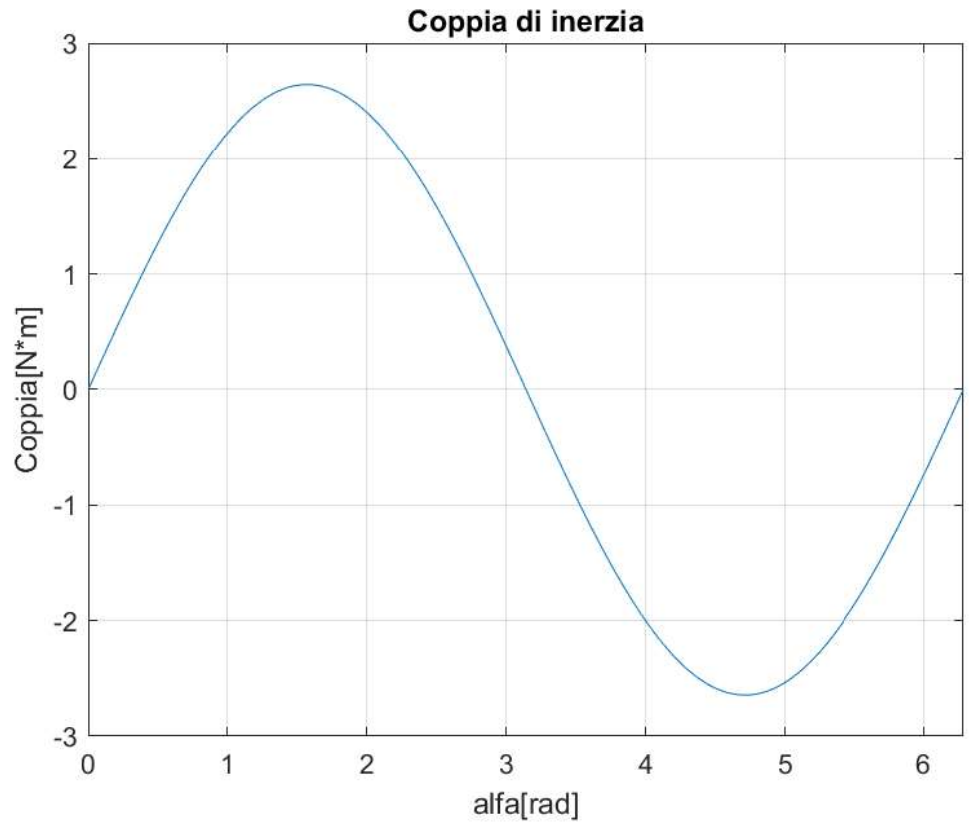
\includegraphics[width=.48\textwidth]{Immagini/GraficoCoppiaInerzia.png}} \quad
   {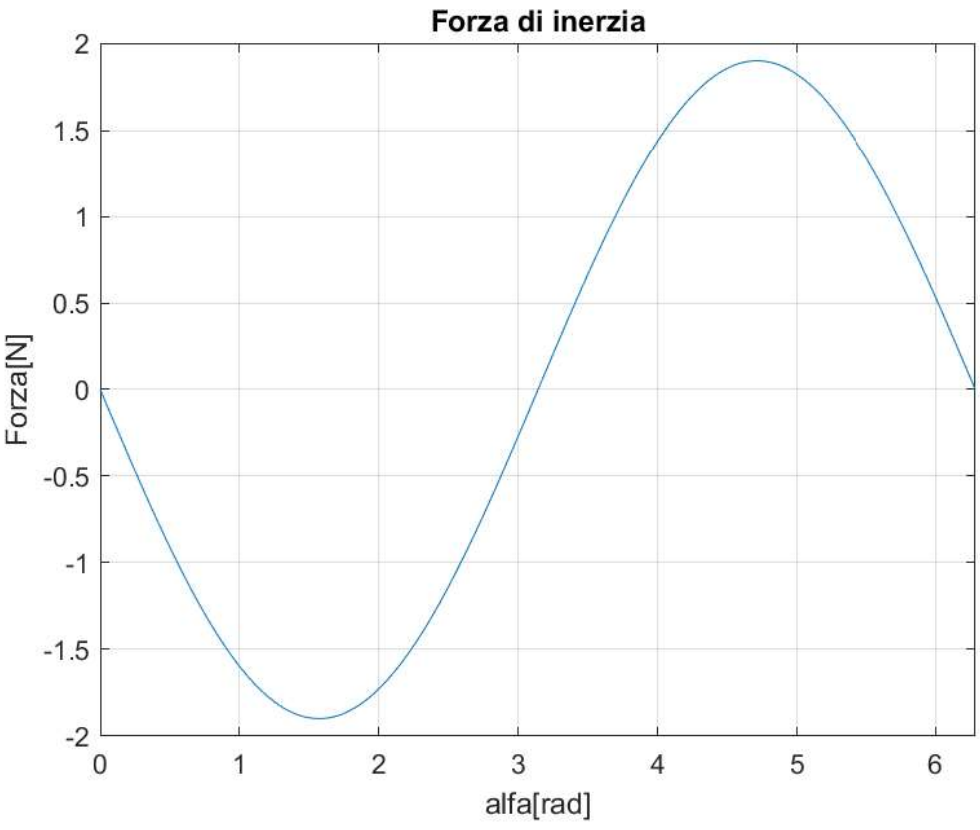
\includegraphics[width=.48\textwidth]{Immagini/GraficoForzaInerzia.png}}
\caption{Andamento della coppia e forza di inerzia al variare di $\alpha$}
\label{fig:GraficoInerziaBiella}
\end{figure}
\begin{lstlisting}[frame=trBL]
%Grafico coppia di inerzia
alfa=linspace(0,2*pi,2000);
Coppiainerzia=-Jo*lambda*w^2*(sin(alfa))
plot(alfa,Coppiainerzia);
xlabel('alfa[rad]'),ylabel('Coppia[N*m]'),
      title('Coppia di inerzia'),grid on,xlim([0 2*pi]);

%Grafico forza di inerzia
Finerzia=Jo*(r/(l^2))*(w^2)*sin(alfa);
plot(alfa,Finerzia);
xlabel('alfa[rad]'),ylabel('Forza[N]'),
      title('Forza di inerzia'),grid on,xlim([0 2*pi]);
\end{lstlisting}
\newpage
\subsubsection{Albero a gomiti}
\paragraph{Forza di inerzia centrifughe}
Le forze di inerzia centrifughe attorno all’asse di rotazione dell’albero corrispondono alle stesse agenti sulla testa di biella, calcolate in precedenza.\\
Quindi $F_c=345,2\ N$.\\
Tuttavia in questo caso, essendoci due manovelle sfasate tra loro di 180°, si formerà una coppia di forze rotanti di medesimo modulo, verso opposto e con rette di applicazioni non appartenenti allo stesso piano ortogonale all’asse.\\
Per tale motivo l’albero sarà equilibrato alle forze alterne del I ordine (traslazione), ma non al momento, manifestando un fenomeno di beccheggio durante il funzionamento. 
\begin{figure}[h]
\centering
   {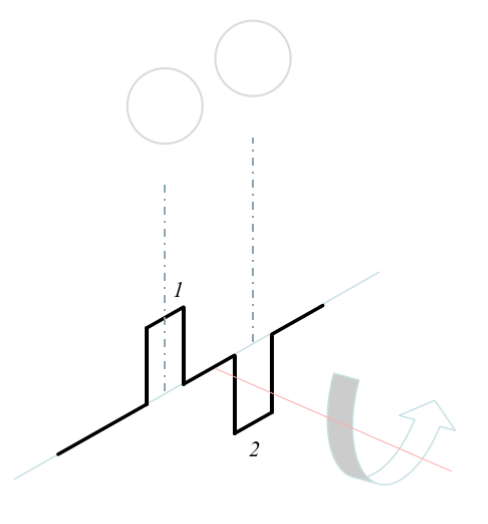
\includegraphics[width=.3\textwidth]{Immagini/Equilibratura1.png}} \quad
   {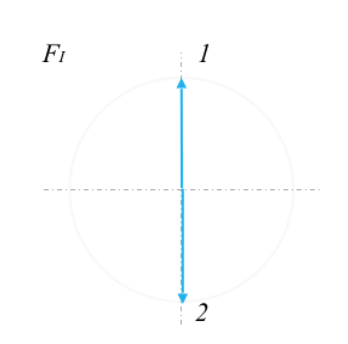
\includegraphics[width=.35\textwidth]{Immagini/Equilibratura2.png}}
\caption{Equilibratura albero a gomiti}
\label{fig:Equilibratura}
\end{figure}
\paragraph{Reazioni scaricate dalla biella sull'albero}Le forze che agiscono su pistone, spinotto e biella si scaricano sull’albero, secondo l’andamento trovato in precedenza (Fig.\ref{fig:GraficoForzaRisultante}).\\
Essendo doppi gli elementi del cinematismo di spinta, in totale sull’albero agiranno due azioni uguali, ma sfasate di 180° tra loro.\\
\begin{figure}[h]
    \centering
    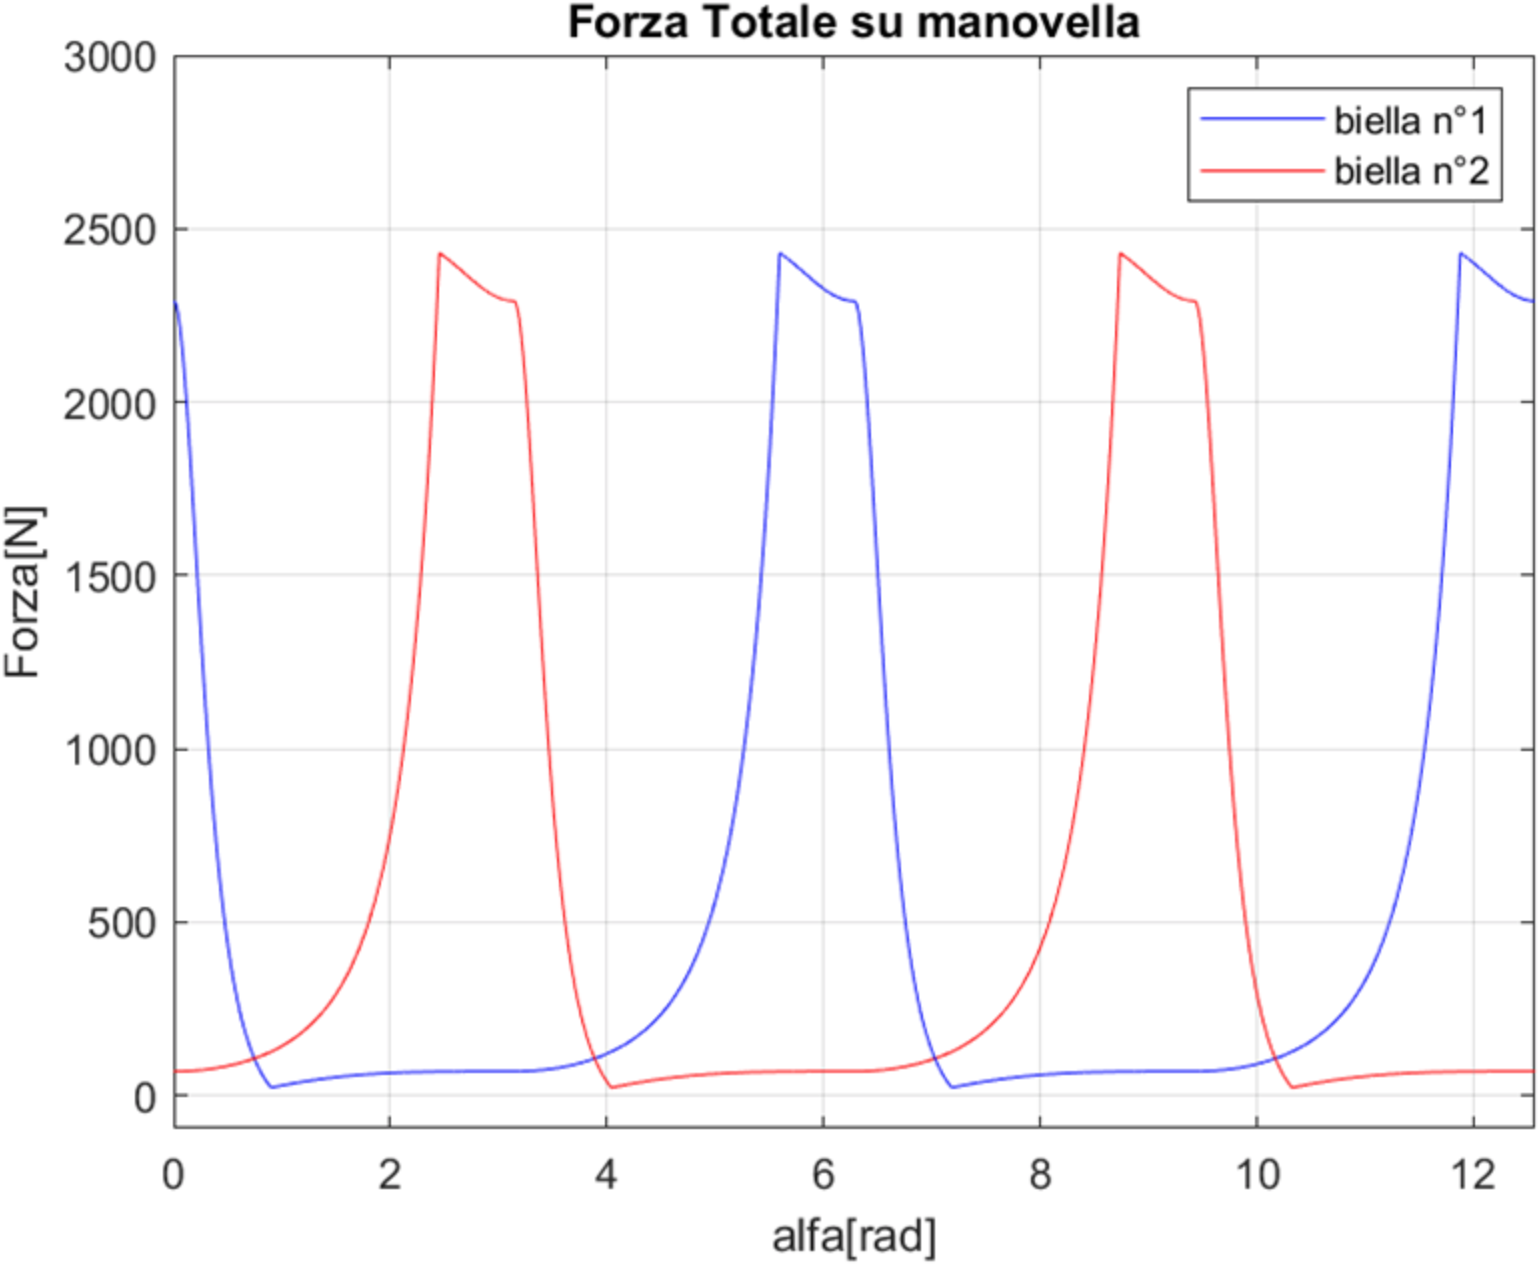
\includegraphics[scale=0.32]{Immagini/GraficoReazioniScaricateAlbero.png}
    \caption{Reazioni scaricate sull'albero al variare di $\alpha$}
    \label{fig:GraficoReazioniScaricateAlbero}
\end{figure}
\subsection{Andamento del momento torcente in funzione dell'angolo di manovella}
Per calcolare il momento torcente sarà necessario identificare la forza $F_{PB}$ ricavata a partire dalla forza totale, precedentemente ricavata, $F_{tot}$ agente sul pistone:
\begin{equation}
    F_{PB}=\frac{F_{tot}}{\cos\beta}
\end{equation}
\begin{figure}[h]
    \centering
    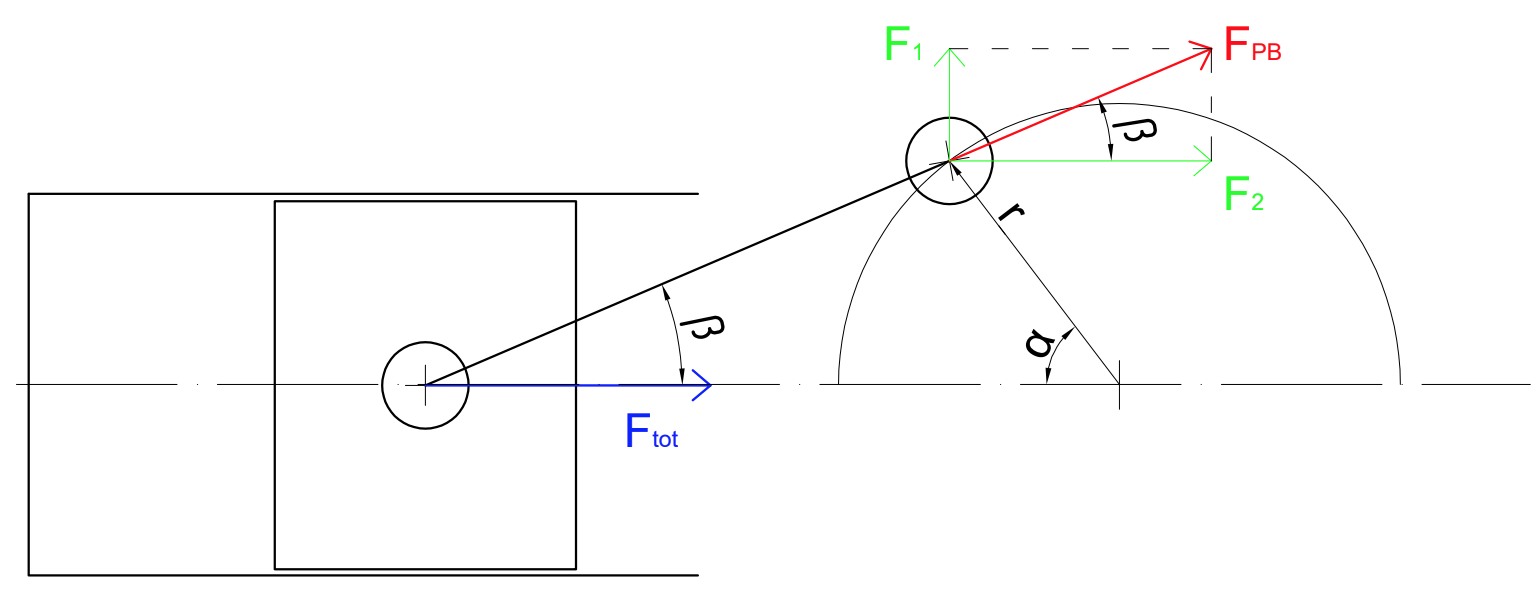
\includegraphics[scale=0.4]{Immagini/SchemaBiellaManovella.png}
    \caption{Schematizzazione delle forze di contributo al momento torcente}
    \label{fig:SchemaBiellaManovella}
\end{figure}
\\
Per quantificare il momento generato da tale forza attorno all’asse di rotazione sarà necessario scomporla in due componenti $F_1$ (ortogonale all’asse di moto del pistone) e $F_2$ (parallela all’asse di moto del pistone).
\begin{equation}
    F_2=F_{PB}\cos\beta
\end{equation}
\begin{equation}
    F_1=F_{PB}\sin\beta
\end{equation}
Ricavate queste componenti sarà quindi possibile calcolare i momenti, noti i rispettivi bracci d’azione.
\begin{equation}
    M_1=F_1r\cos\alpha
\end{equation}
\begin{figure}[h]
    \centering
    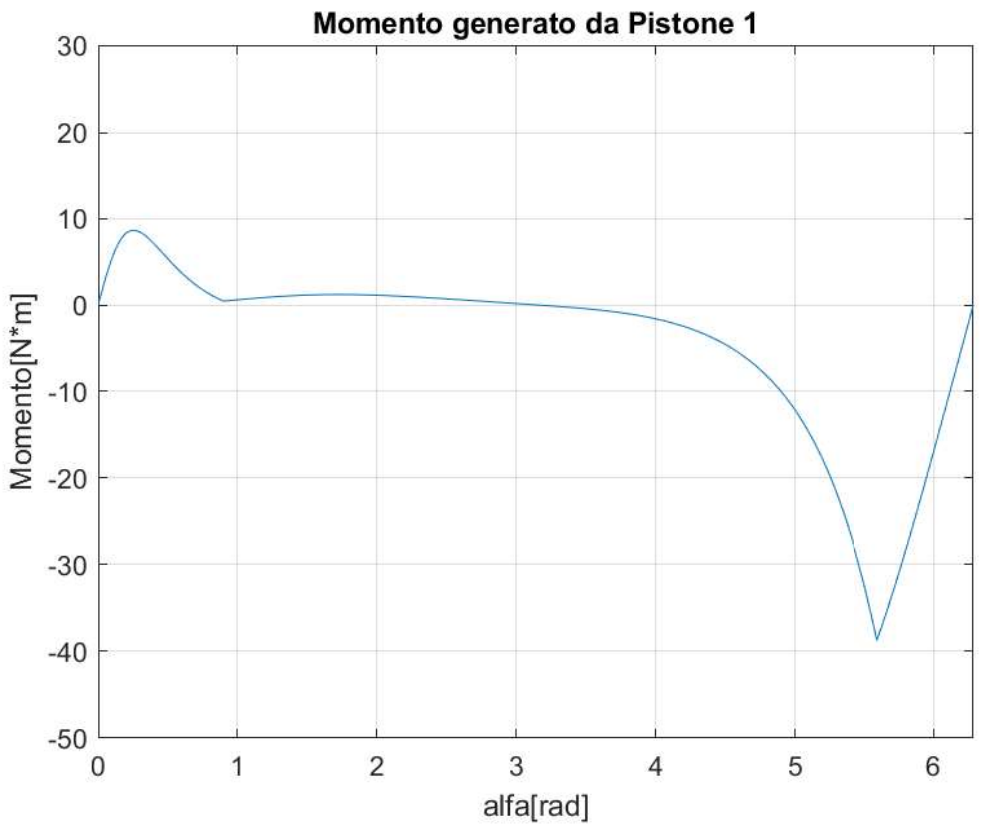
\includegraphics[scale=0.45]{Immagini/GraficoMomento1.png}
    \caption{Andamento del momento torcente generato dal primo cilindro}
    \label{fig:GraficoMomento1}
\end{figure}
\newpage
L’immagine di Fig.\ref{fig:GraficoMomento1} mostra l’andamento del momento torcente sull’albero a gomiti dovuto alle forze di pressione, all’inerzia del pistone, spinotto, testa e piede di biella. 
\begin{lstlisting}[frame=trBL]
%Grafico Momento torcente cilindro 1

senbeta=r/l*sin(alfatot);
cosbeta=sqrt(1-senbeta.^2);
Forzatrasmessa=Ftot./cosbeta;
F1=Forzatrasmessa.*senbeta;
F2=Forzatrasmessa.*cosbeta;
Mt1=r.*cos(alfatot).*F1+r.*sin(alfatot).*F2;
plot(alfatot,Mt1,'b');
xlabel('alfa[rad]'),ylabel('Momento[N*m]'),
      title('Momento generato da Pistone 1'),
      grid on,xlim([0 2*pi]),ylim([-50 50]);
\end{lstlisting}
L’andamento del momento torcente dovuto all’azione del secondo cilindro sarà uguale in modulo a quello ottenuto per il primo (Fig.\ref{fig:GraficoMomento1}), ma sfasato di 180°. 
\begin{equation}
    M_2=F_2r\sin\alpha
\end{equation}
\begin{figure}[h]
    \centering
    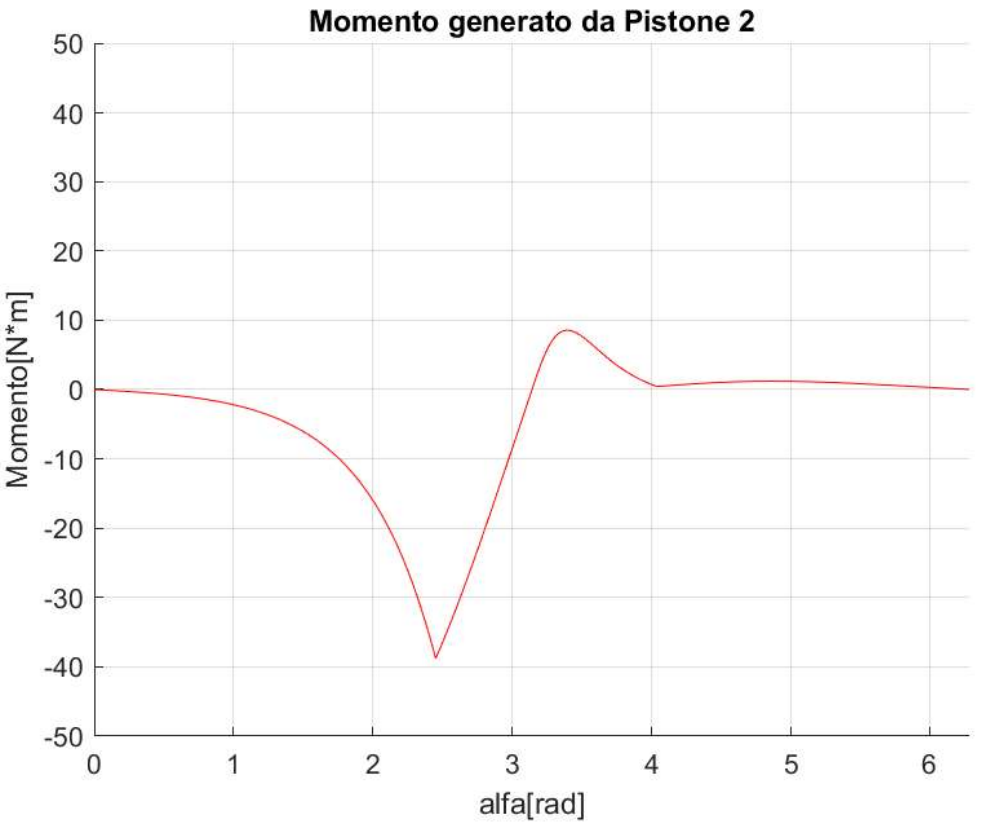
\includegraphics[scale=0.45]{Immagini/GraficoMomento2.png}
    \caption{Andamento del momento torcente generato dal secondo cilindro}
    \label{fig:GraficoMomento2}
\end{figure}
\begin{lstlisting}[frame=trBL]
%Momento torcente pistone 2

alfatot2=alfatot+3.14;
senbeta2=r/l*sin(alfatot2);
cosbeta2=sqrt(1-senbeta2.^2);
F12=Forzatrasmessa.*senbeta2;
F22=Forzatrasmessa.*cosbeta2;
Mt2=+r.*cos(alfatot2).*F12-r.*sin(alfatot2).*F22;
plot(alfatot2,Mt2,'r');
hold on
plot(alfatot2-2*pi,Mt2,'r');

xlabel('alfa[rad]'),ylabel('Momento[N*m]'),
      title('Momento generato da Pistone 2'),
      grid on,xlim([0 2*pi]),ylim([-50 50]);
\end{lstlisting}
In aggiunta bisognerebbe considerare anche il contributo in termini di momento dovuto alle forze derivanti dal momento di inerzia della biella J:
\begin{equation}
    M_{ci}=F_{ci}r\cos\alpha
\end{equation}
con $F_{ci}$ da eq.(\ref{ForzaCoppiaBiella}), il cui andamento era già stato riportato in Fig.\ref{fig:GraficoInerziaBiella}.
\begin{figure}[h]
    \centering
    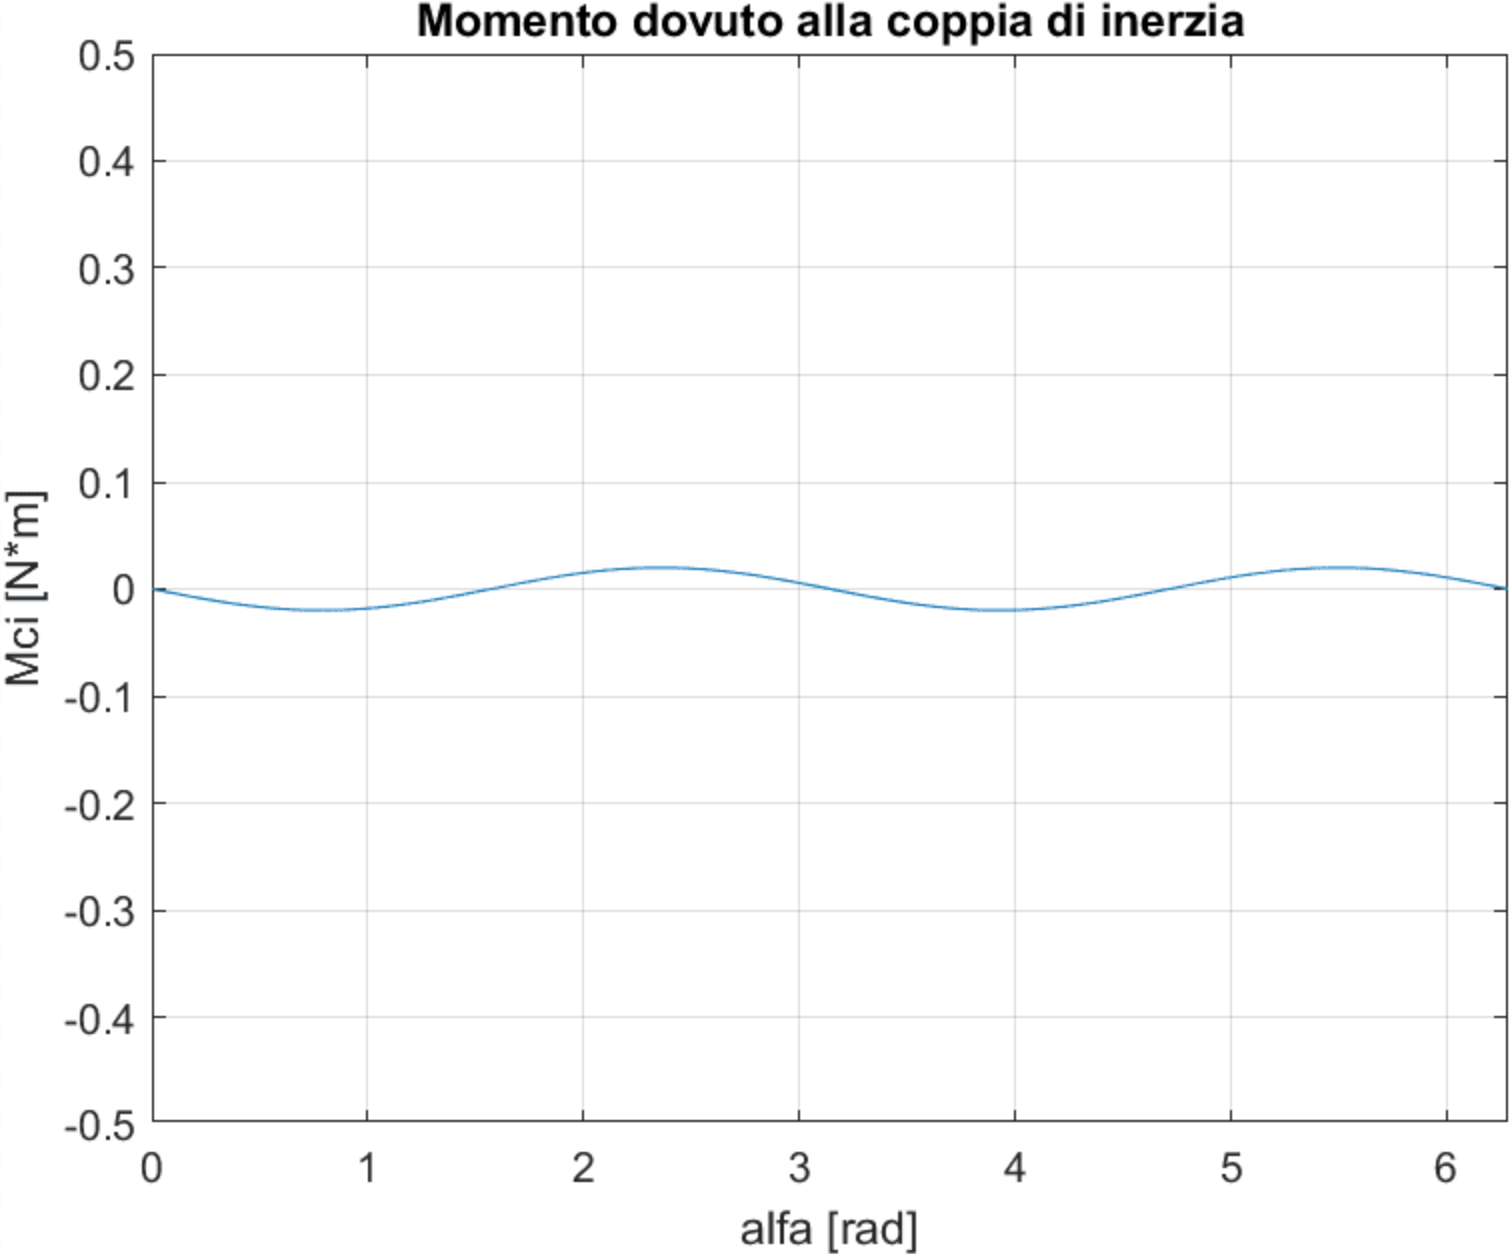
\includegraphics[scale=0.3]{Immagini/GraficoMomentoCoppiaBiella.png}
    \caption{Andamento del momento torcente dovuto alle forze di inerzia della biella}
    \label{fig:GraficoMomentoCoppiaBiella}
\end{figure}
\begin{lstlisting}[frame=trBL]
% Momento torcente dovuto alla coppia di inerzia della biella

Mci=Finerzia*r.*cos(alfa);
plot(alfa,Mci);
xlabel('alfa [rad]'),ylabel('Mci [N*m]'),
      title('Momento dovuto alla coppia di inerzia'),
      grid on, xlim([0 2*pi]),ylim([-0.5 0.5]);
\end{lstlisting}
Com’è possibile osservare dal grafico ottenuto in Matlab questo contributo risulta trascurabile in termini quantitativi rispetto ad $M_1$ ed $M_2$.\\
Quindi questo contributo non sarà tenuto in considerazione nemmeno per il momento torcente complessivamente generato sull'albero a gomiti. \\
In fase di calcolo si terrà comunque conto indirettamente di questo contributo, assumendo un minimo coefficiente di sicurezza, che contempli il fatto che il momento potrebbe essere leggermente superiore rispetto al valore considerato.\\
\\
Di seguito vengono riportati i due andamenti precedentemente ottenuti all’interno di un unico grafico.
\begin{figure}[h]
    \centering
    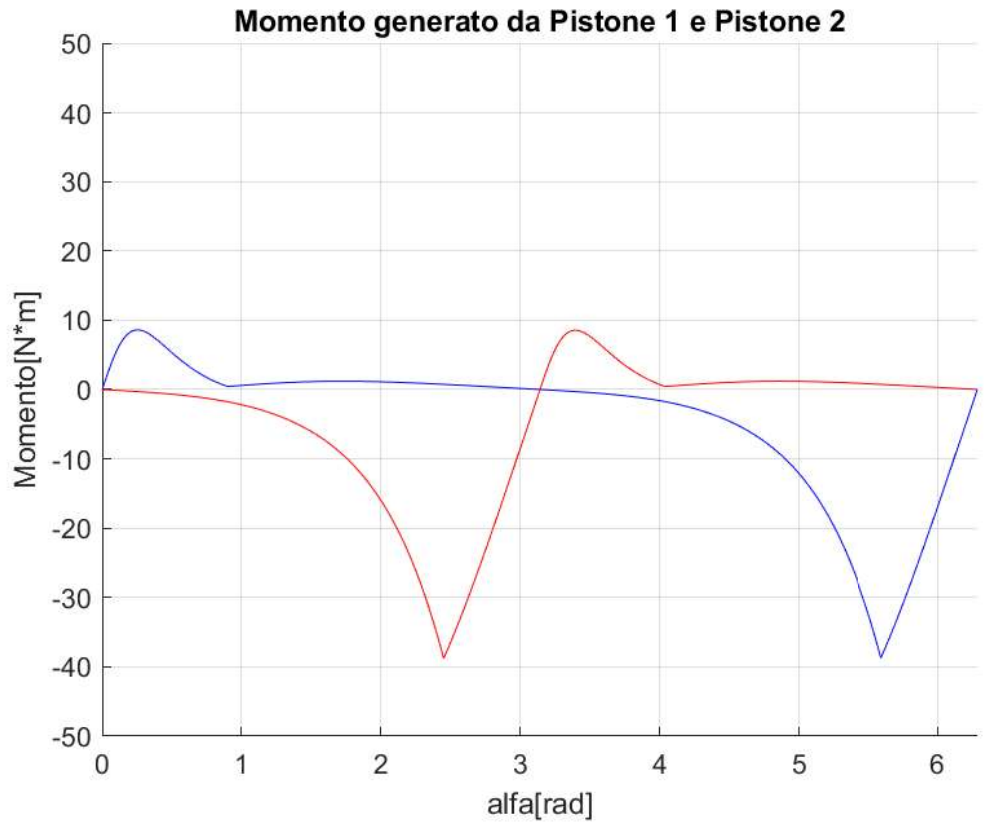
\includegraphics[scale=0.5]{Immagini/GraficoMomento1e2.png}
    \caption{Andamento dei due momenti generati all'interno di un unico giro di manovella}
    \label{fig:GraficoMomento1e2}
\end{figure}
\begin{lstlisting}[frame=trBL]
%%Momento torcente dei due pistoni insieme

%Momento torcente pistone 1
senbeta=r/l*sin(alfatot);
cosbeta=sqrt(1-senbeta.^2);
Forzatrasmessa=Forzaris./cosbeta;
F1=Forzatrasmessa.*senbeta;
F2=Forzatrasmessa.*cosbeta;
Mt1=r.*cos(alfatot).*F1+r.*sin(alfatot).*F2;
plot(alfatot,Mt1,'b');

hold on       %del momento torcente 1

%Momento torcente pistone 2
alfatot2=alfatot+3.14;
senbeta2=r/l*sin(alfatot2);
cosbeta2=sqrt(1-senbeta2.^2);
F12=Forzatrasmessa.*senbeta2;
F22=Forzatrasmessa.*cosbeta2;
Mt2=+r.*cos(alfatot2).*F12-r.*sin(alfatot2).*F22;
plot(alfatot2,Mt2,'r');
hold on       %del momento torcente 2
plot(alfatot2-2*pi,Mt2,'r');

xlabel('alfa[rad]'),ylabel('Momento[N*m]'),
      title('Momento generato da Pistone 1 e Pistone 2'),
      grid on,xlim([0 2*pi]),ylim([-50 50]);

hold off       %dei due momenti torcenti
\end{lstlisting}
Il momento torcente totale relativo ai due cilindri sarà definito come:
\begin{equation}
    M=M_1+M_2.
\end{equation}
\begin{figure}[h]
    \centering
    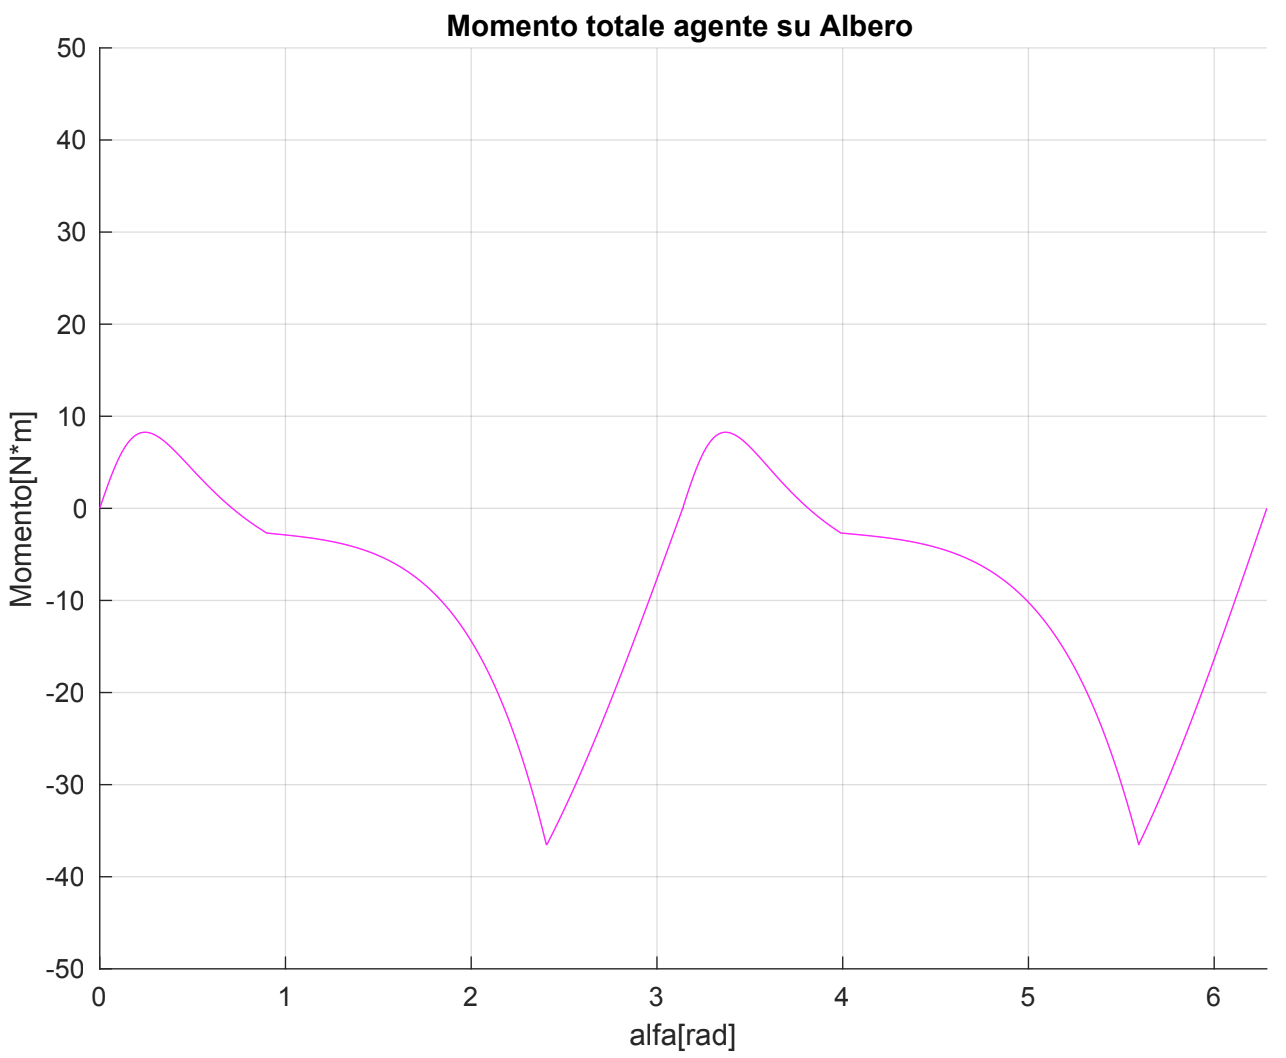
\includegraphics[scale=0.4]{Immagini/GraficoMomentoTotale.png}
    \caption{Andamento del momento torcente risultate sull'albero a gomiti}
    \label{fig:GraficoMomentoTotale}
\end{figure}
\begin{lstlisting}[frame=trBL]
%Grafico momento torcente totale

Mt2=circshift(Mt1,1000); %shifta il vettore Mt1 
                         %di meta dei valori (1000)
Mttot=Mt1+Mt2;
plot(alfatot,Mttot,'m');
xlabel('alfa[rad]'),ylabel('Momento[N*m]'),
      title('Momento totale agente su albero'),
      grid on,xlim([0 2*pi]),ylim([-50 50])
\end{lstlisting}
\subsection{Determinazione del volano che regolarizza il momento torcente}
Il volano ha il compito di assorbire l’eccesso di lavoro resistente rispetto a quello motore, sotto forma di energia cinetica, evitando che si verifichino incrementi di velocità angolare non compatibili con l’impiego a cui il sistema è destinato. \\
Come già mostrato, in Fig.\ref{fig:GraficoMomentoTotale} è riportato il momento resistente del compressore bicilindrico in esame. \\
Quando il momento resistente medio $M_{rm}$ è uguale al momento motore $M_m$, la velocità di rotazione media $\omega$ rimane costante, ma nell’intervallo in cui il momento resistente effettivo è maggiore del momento motore, la velocità istantanea di rotazione diminuisce (e quando il momento resistente è minore del momento motore, la velocità istantanea tende ad aumentare). 
\begin{figure}[h]
    \centering
    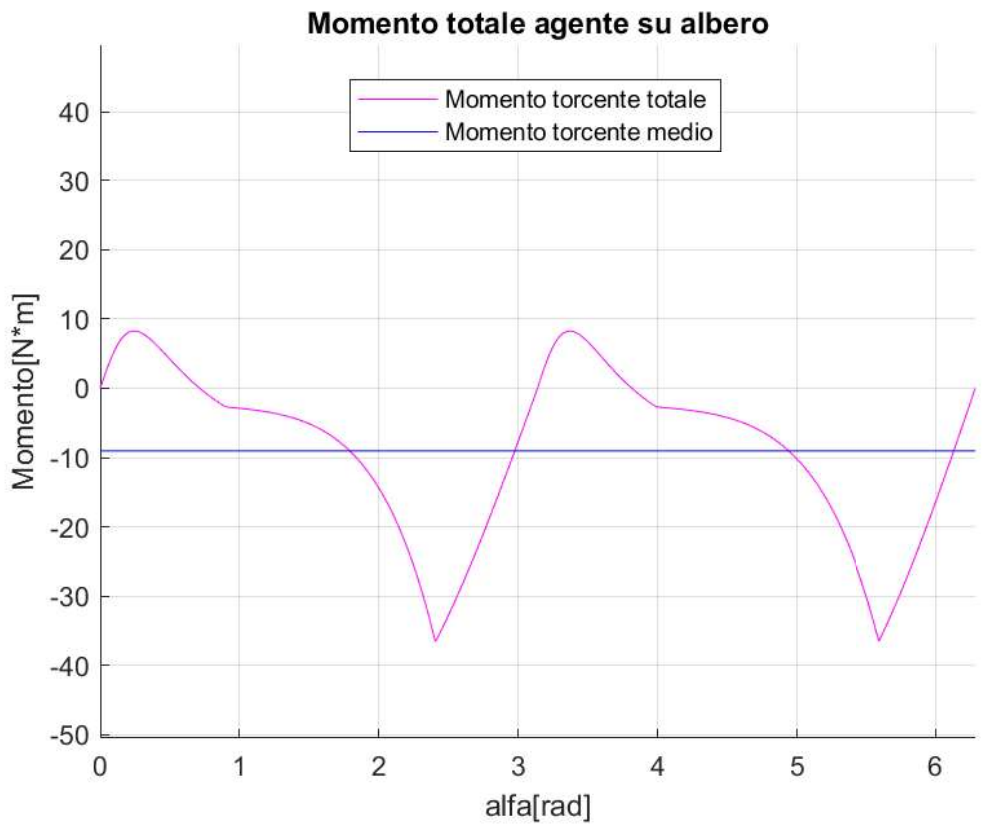
\includegraphics[scale=0.5]{Immagini/GraficoMomentoMedio.png}
    \caption{Confronto andamento momento torcente con momento torcente medio}
    \label{fig:GraficoMomentoMedio}
\end{figure}
\begin{lstlisting}[frame=trBL]
%Momento torcente medio

m=mean(Mttot); %trova la media
s=linspace(m,m,2000);
plot(alfatot,s,'b')
hold off %il vecchio grafico era stato tenuto in 
         %plot con comando hold on
\end{lstlisting}
\paragraph{Grado di irregolarità e lavoro eccedente}Indicando con $\omega_2$ la massima velocità nel periodo e con $\omega_1$ la minima, è possibile ricavare la la velocità mediante: 
\begin{equation}
    \omega=\frac{\left(\omega_1+\omega_2\right)}{2}.
\end{equation}
Si definisce grado di irregolarità nel periodo il rapporto tra la variazione di velocità e la velocità media: 
\begin{equation}
    \delta=\frac{\omega_2-\omega_1}{\omega}
\end{equation}
Da tabella I.141 del Manuale di meccanica Hoepli si stima $\delta=0.03$, relativo alle trasmissioni da officina.
\paragraph{Calcolo del momento di inerzia del volano}
Indicando con N [W] la potenza e con n [giri/min] i giri al minuto dell’albero motore, si ha:
\begin{equation}
    N=M_{rm}\omega=M_{rm}\frac{2\pi n}{60}
\end{equation}
da cui si può ricavare il lavoro medio in un giro: 
\begin{equation}
    M_{rm}2\pi=60\frac{N}{n}.
    \label{LavoroMedioGiro}
\end{equation}
Il lavoro massimo di fluttuazione risulta essere pari a: 
\begin{equation}
    L_F=\int_{\alpha_A}^{\alpha_B}{(M_r-}M_{rm})d\alpha\ =\frac{1}{2}I\left(\omega_2^2-\omega_1^2\right)
    \label{LavoroFluttuazione}
\end{equation}
dove I rappresenta il momento di inerzia di tutte le masse rotanti rispetto all’asse di rotazione.\\
\begin{figure}[h]
    \centering
    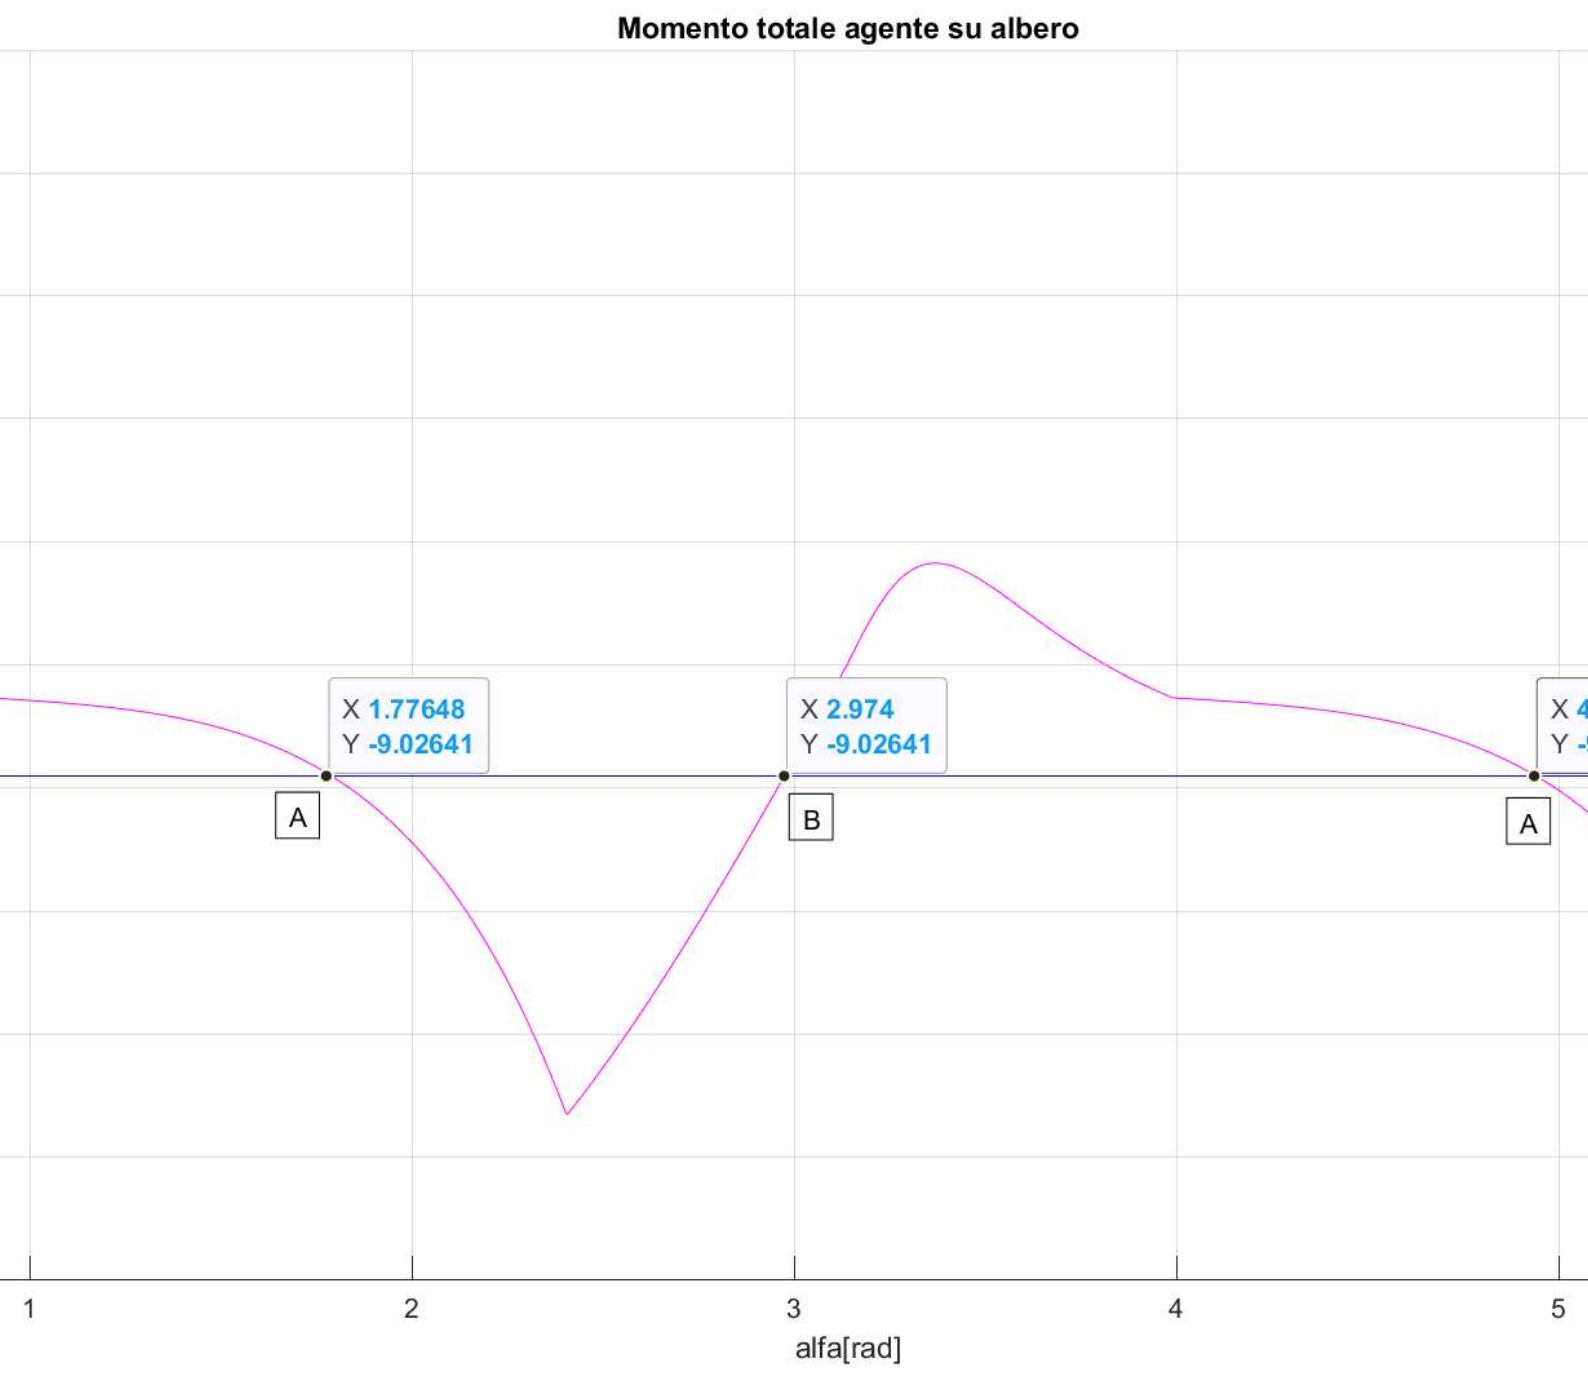
\includegraphics[scale=0.3]{Immagini/GraficoPuntiMomento.png}
    \caption{Punti A e B indicati in formula \ref{LavoroFluttuazione}}
    \label{fig:GraficoPuntiMomento}
\end{figure}
\\
In prima approssimazione si ritiene preponderante il momento di inerzia del volano rispetto alle altre masse e, quindi, nella trattazione I sarà il momento di inerzia del volano.\\
\\
Concretamente il lavoro massimo di fluttuazione corrisponde alla massima area sottesa tra la curva del momento resistente $M_r$ e il suo valore medio $M_{rm}$.\\
Esso può essere anche espresso come frazione del lavoro medio in un giro: 
\begin{equation}
    L_F=\varphi M_r2\pi=\varphi\ 60\frac{N}{n}
    \label{FrazioneLavoroMedio}
\end{equation}
in cui $\varphi$ è il coefficiente di fluttuazione, dipendente dal tipo di applicazione e ricavabile tramite tabelle. \\
Per i successivi calcoli considereremo un $\varphi$ pari a 0,15. 
\paragraph{Calcolo momento di inerzia del volano}Tenendo conto delle eq.(\ref{FrazioneLavoroMedio}), (\ref{LavoroFluttuazione}) e (\ref{LavoroMedioGiro}), può essere scritta:
\begin{equation}
    \varphi\ 60\frac{N}{n}=I\omega^2
\end{equation}
da cui si può ricavare il momento di inerzia del volano in funzione della potenza, del coefficiente di fluttuazione e del grado di irregolarità:
\begin{equation}
    I=\frac{2\pi\varphi N}{\delta \omega^3}.
\end{equation}
Facendo i calcoli si ottiene che $I=\left|10,9\cdot10^{-3}\right|\ kgm^2$. 
Noto il raggio del volano pari a $r=150\ mm$, è possibile determinare la massa del volano come: 
\begin{equation}
    m=\frac{I}{r^2}=0,5\ kg.
\end{equation}
I risultati ottenuti sono compatibili con quelli ricavati mediante SOLIDWORKS.
\begin{figure}[h]
    \centering
    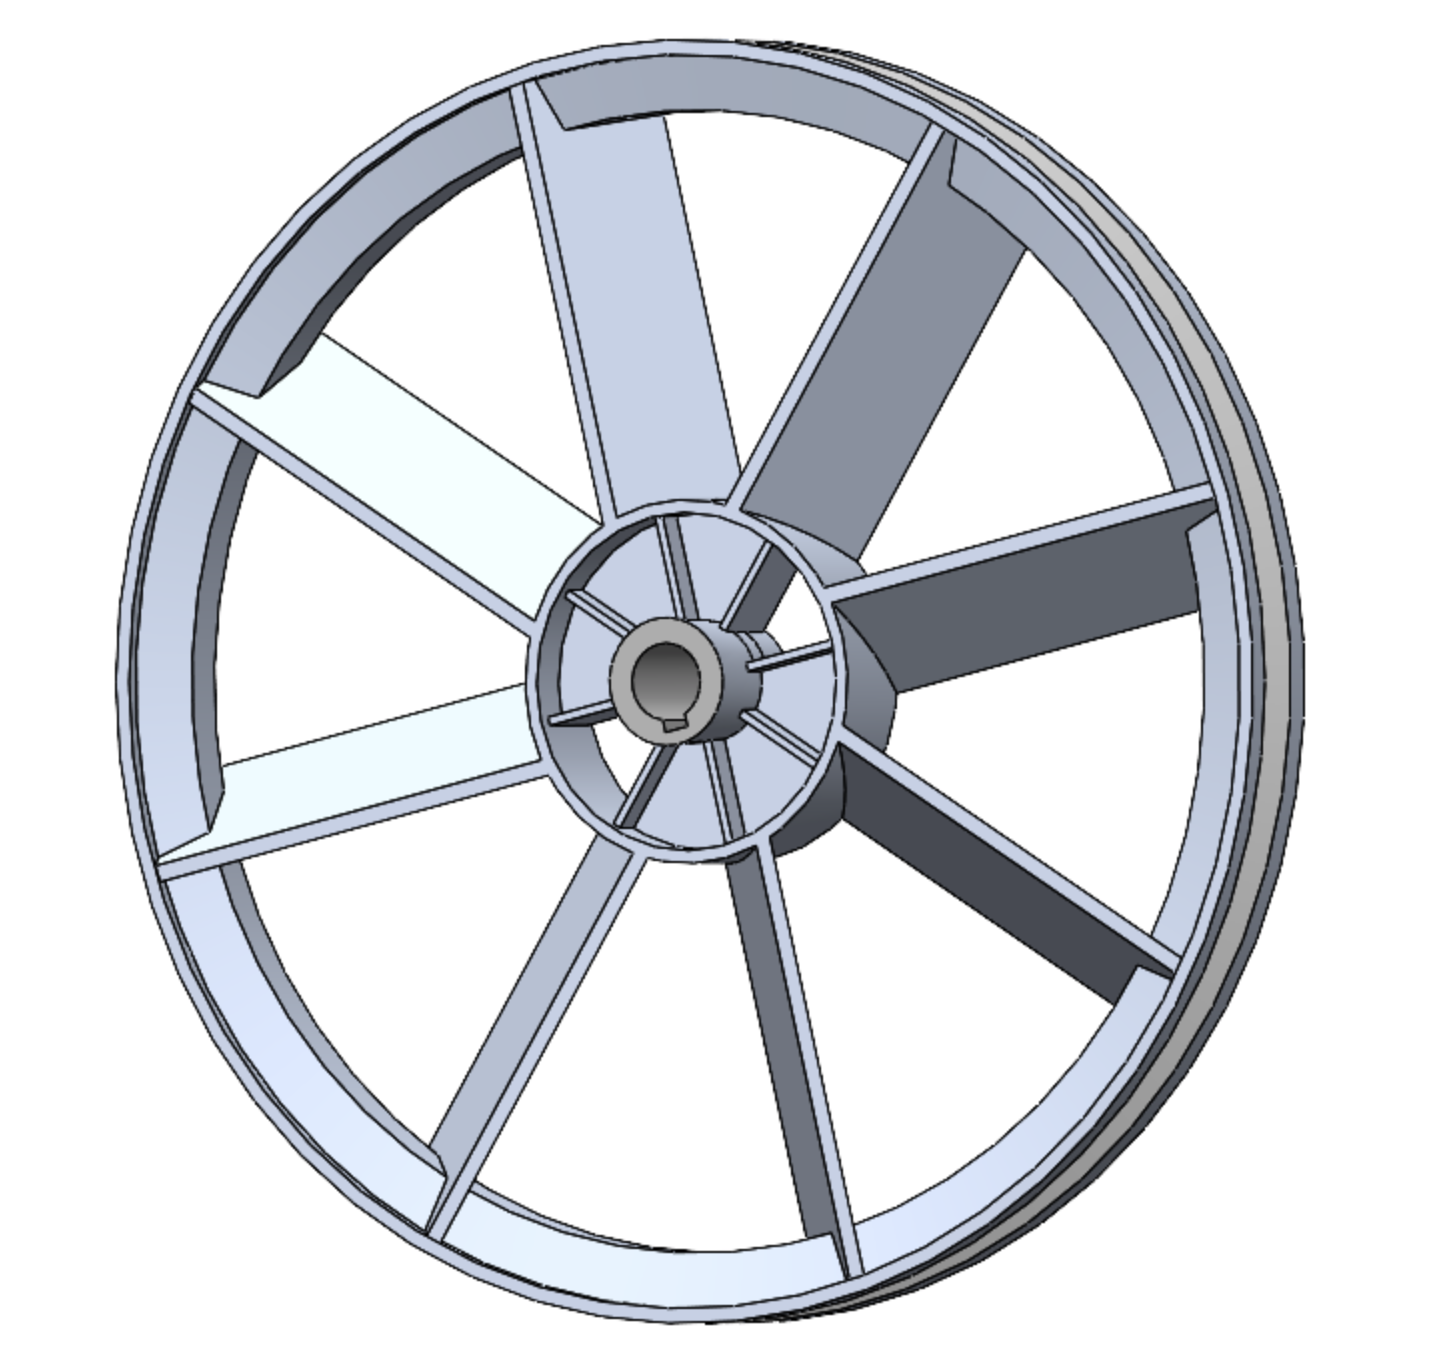
\includegraphics[scale=0.2]{Immagini/Volano.png}
    \caption{Modello CAD SOLIDWORKS del volano}
    \label{fig:Volano}
\end{figure}
\begin{figure}[h]
    \centering
    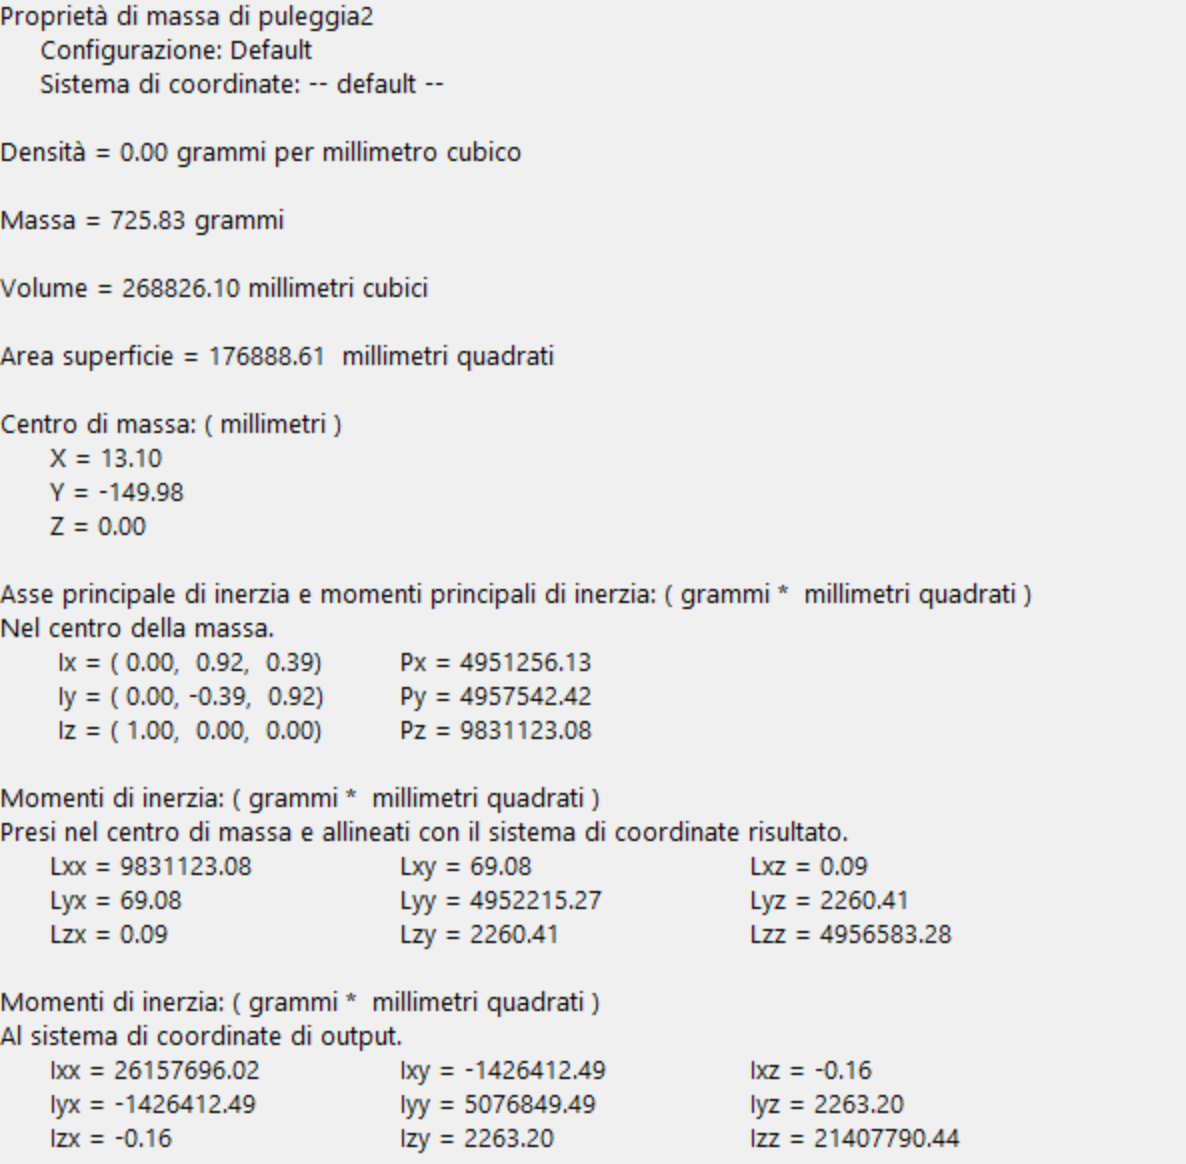
\includegraphics[scale=0.5]{Immagini/CaratteristicheVolano.png}
    \caption{Caratteristiche del volano ricavate mediante software SOLIDWORKS}
    \label{fig:CaratteristicheVolano}
\end{figure}
\newpage
È possibile, inoltre, determinare la velocità periferica dei punti più esterni della corona che non può superare limiti ben precisi, per non creare eccessive sollecitazioni nel materiale.\\
Nella maggior parte dei casi si tende a mantenere tale velocità intorno ai 30 - 35 m/s. Nel caso specifico in esame si ottiene una velocità periferica pari a:
\begin{equation}
    v=\omega r=24,25\ m/s
\end{equation}
rientrante nel range di sicurezza. 
\subsection{Determinazione del motore elettrico}
Noto il valore medio del momento resistente, sarà possibile determinare la potenza motrice richiesta per il funzionamento del compressore alla macchina elettrica: 
\begin{equation}
    N=M_{rm}\omega=1454,64\ W=1,45\ kW.
\end{equation}
Considerando un rendimento complessivo della trasmissione a cinghia pari a $\eta=0,96$ si ottiene che la potenza che il motore deve complessivamente fornire corrisponde a: 
\begin{equation}
    N_{eff}=\frac{N}{\eta}=1,5\ kW.
\end{equation}
Da catalogo Nuova Omas è stato scelto un motore con caratteristiche idonee. 
\begin{figure}[h]
    \centering
    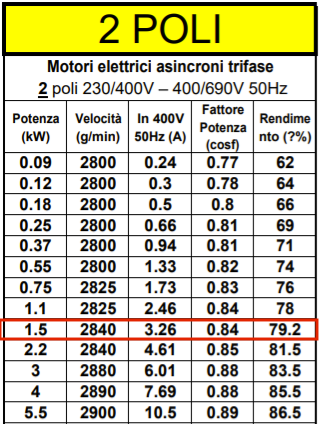
\includegraphics[scale=0.6]{Immagini/CatalogoMotoreElettrico.png}
    \caption{Catalogo Nuova Omas per la scelta del motore elettrico}
    \label{fig:CatalogoMotoreElettrico}
\end{figure}
\subsection{Calcolo della trasmissione con cinghia trapezoidale}
Le cinghie trapezoidali sono così chiamate per la forma della loro sezione, che si presenta come nella figura sottostante (Fig.\ref{fig:CinghiaTrapezoidale}).
\newpage
\begin{figure}[h]
    \centering
    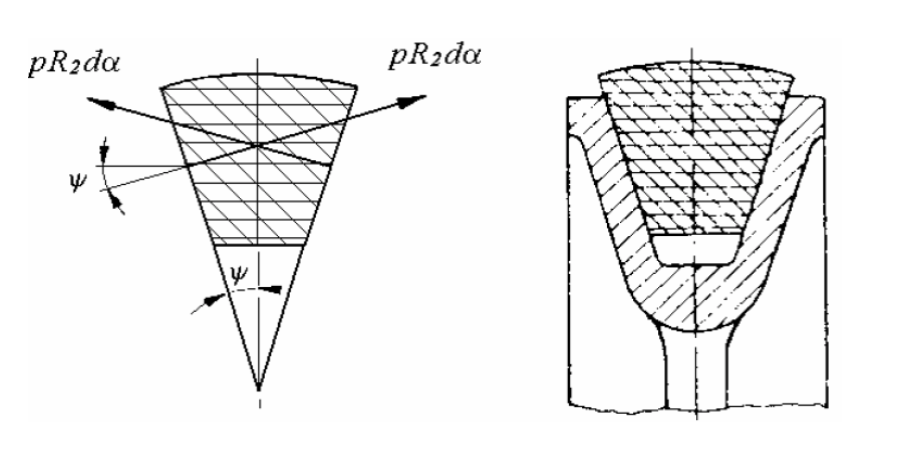
\includegraphics[scale=0.4]{Immagini/CinghiaTrapezoidale.png}
    \caption{Vista di una cinghia trapezoidale in sezione}
    \label{fig:CinghiaTrapezoidale}
\end{figure}
La cinghia è costruita in elastomero, con uno o più strati di trefoli in poliestere ed un rivestimento esterno protettivo di tela impregnata con elastomero. Il materiale con cui la cinghia è realizzata permette di raggiungere elevati coefficienti di attrito, ma è soprattutto il modo con  cui essa esercita la sua azione sulla puleggia, che contribuisce ad accrescere l’attrito con quest’ultima (contatto con le superfici laterali di una gola a V).\\
Le cinghie di trasmissione trapezoidali sono le più utilizzate per la trasmissione di potenza, perché risolvono allo stesso tempo il problema dell’allineamento e parzialmente dello slittamento. \\
Se le potenze in gioco sono elevate, è possibile utilizzare sulla stessa puleggia (con scanalature multiple) più cinghie trapezoidali.\\
\\
I dati fino ad ora noti ed indispensabili per la progettazione del sistema di trasmissione sono: 
\begin{itemize}
    \item Velocità di rotazione albero a gomiti: $n = n_2 = 1540\ rpm$ 
    \item Velocità di rotazione albero motore elettrico: $n_1 = 2840\ rpm$
    \item Diametro esterno puleggia compressore: $d_{2e} = 300\ mm$
    \item Diametro interno puleggia compressore: $d_{2i} = 274\ mm$
    \item Diametro medio puleggia compressore: $d_{2m}=\frac{d_{2e}+d_{2i}}{2}=287\ mm$
    \item Potenza trasmessa: $P = 1,5\ kW$
    \item Velocità periferica media puleggia compressore: $v_{2m}=\frac{2\pi n_2}{60}\ \frac{d_{2m}}{2}=23,14\ m/s$ (gamma di velocità ottimale varia fra i 5 e i 50 m/s).
\end{itemize}
\begin{figure}[h]
    \centering
    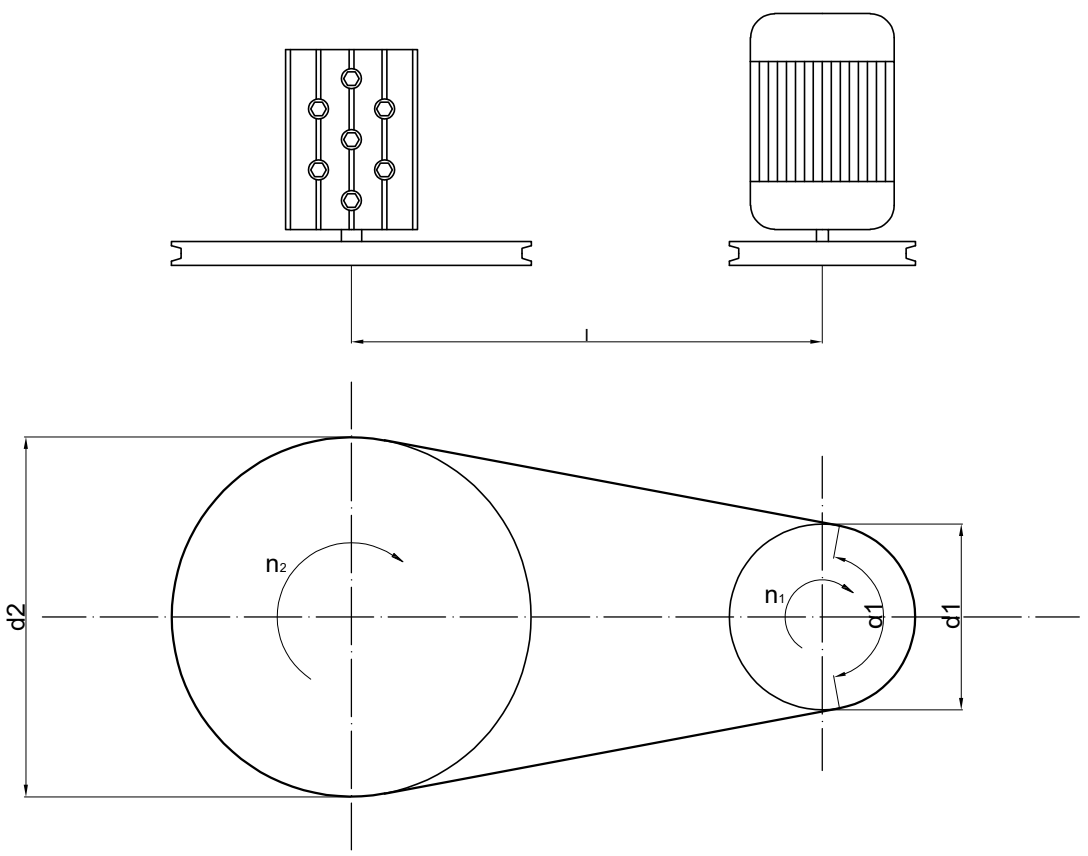
\includegraphics[scale=0.55]{Immagini/SchemaMontaggio.png}
    \caption{Schema di montaggio delle pulegge}
    \label{fig:SchemaMontaggio}
\end{figure}
Note le velocità di rotazione del motore elettrico e dell’albero motore del compressore, è possibile stimare il rapporto di trasmissione del sistema meccanico come:
\begin{equation}
    \tau=\frac{n_2}{n_1}=1,844
\end{equation}
da cui è possibile ricavare il diametro medio della puleggia associata alla macchina elettrica, ovvero quella più piccola:
\begin{equation}
    d_{1m}=\frac{d_{2m}}{\tau}=155,6\ mm.
\end{equation}
Ottenuti questi parametri si può quindi procedere nella progettazione della trasmissione a cinghia trapezoidale, riferendosi alle procedure indicate sul catalogo Pi Belt Pizzirani. \\
Si inizia supponendo un opportuno interasse tra le due pulegge scelto fra un range di valori raccomandati, in funzione dei diametri medi delle due pulegge. 
\begin{equation}
    0,7(d_{1m}+d_{2m})<I<2(d_{1m}+d_{2m})=309,83\ mm<I<885,24\ mm\ 
\end{equation}
Si sceglie un interasse teorico pari a $I_{th}=450\ mm$.
Da questo sarà quindi poi possibile determinare la lunghezza complessiva dell’organo flessibile mediante la seguente relazione: 
\begin{equation}
    L_{th}=2I_{th}+1,57\left(d_{1m}+d_{2m}\right)+\frac{\left(d_{2m}-d_{1m}\right)^2}{4 I_{th}}=1604,5\ mm
\end{equation}
Prima di determinare la lunghezza reale della cinghia sarà però necessario determinarne la tipologia costruttiva, in base alle dimensioni note della puleggia reperibili mediante valutazione del disegno su SOLIDWORKS.\\
\begin{figure}[h!]
    \centering
    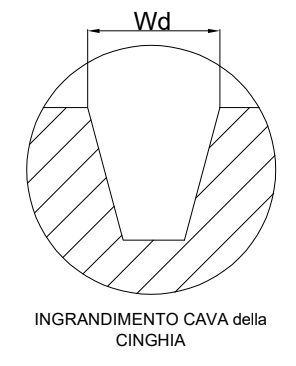
\includegraphics[scale=0.6]{Immagini/IngrandimentoCinghia.png}
    \caption{Ingrandimento della cava della cinghia}
    \label{fig:IngrandimentoCinghia}
\end{figure}

Poiché risulta $W_d=13\ mm$ è stata scelta una cinghia di tipologia B con le caratteristiche dimensionali rappresentate sotto in tabella.\\
\begin{figure}[h]
    \centering
    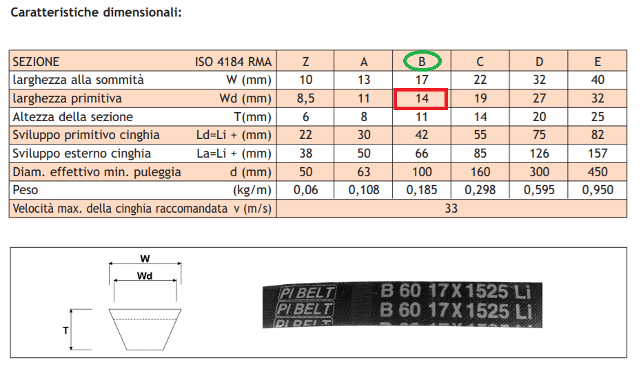
\includegraphics[scale=0.7]{Immagini/CaratteristicheDimensionaliCinghia.png}
    \caption{Dimensionamento cinghia da catalogo}
    \label{fig:CaratteristicheDimensionaliCinghia}
\end{figure}

A questo punto è possibile individuare la lunghezza reale della cinghia, scegliendola sempre dal medesimo catalogo.\\
\newpage
\begin{figure}[h]
    \centering
    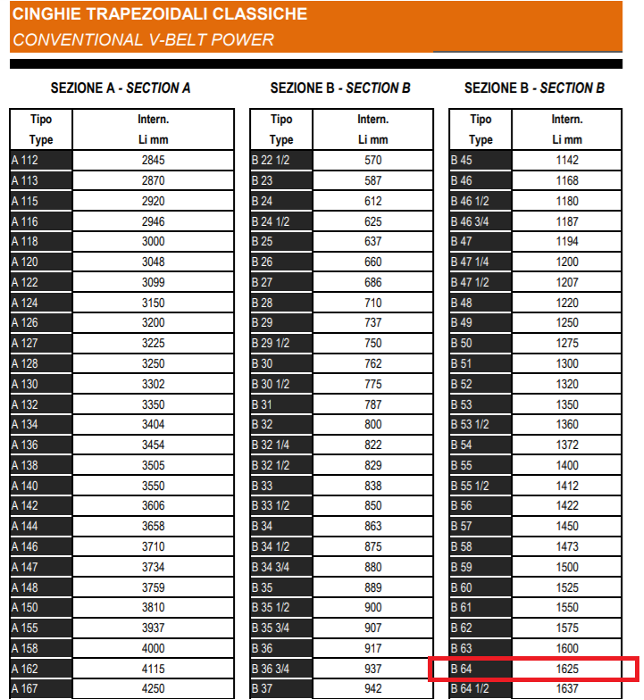
\includegraphics[scale=0.65]{Immagini/SceltaCinghia.png}
    \caption{Selta della cinghia da catalogo}
    \label{fig:SceltaCinghia}
\end{figure}

La cinghia scelta è la B64, con una lunghezza pari a: 
\begin{equation}
    L=1625\ mm.
\end{equation}
Da questa si ricava il valore reale dell’interasse, che inizialmente era solo stato ipotizzato, come: 
\begin{equation}
    I=\frac{L-1,57\left(d_{1m}+d_{2m}\right)}{2}-\frac{\left(d_{2m}-d_{1m}\right)^2}{4\left[L-1,57\left(d_{1m}+d_{2m}\right)\right]}=462\ mm
\end{equation}
Si è quindi caratterizzato dimensionalmente il sistema di trasmissione meccanica a cinghia.\\
\\
Si può poi proseguire con la valutazione del pretensionamento da conferire alla cinghia, per garantire la trasmissione del moto fra le due pulegge evitando slittamenti. 
\paragraph{Calcolo del pretensionamento}Nuovamente dal catalogo è possibile quantificare il valore della forza di pretensionamento da fornire al sistema di trasmissione, come esplicitato dalla seguente relazione: 
\begin{equation}
    T=\frac{50\left(2,5-a\right) P}{a N v_{2m}}+Kv_{2m}^2
\end{equation}
dove: 
\begin{itemize}
    \item a: fattore di correzione dell’arco di contatto (ricavabile dalla Fig.\ref{fig:ArcoDiContatto}) 
    \item K: coefficiente relativo alla massa lineare delle cinghie (ricavabile dalla Fig.\ref{fig:CoefficienteK})
    \item N = numero di pulegge (supposto inizialmente N = 1).
\end{itemize}
Quindi con $a=0.96$, $K=0,019$ e $N=1$ si ottiene una forza di pretensionamento pari a: 
\begin{equation}
    T=52,1\ N.
\end{equation}
Questo pretensionamento T genera sull’albero una forza statica di modulo: 
\begin{equation}
    R_s=2NT\cos\left(90^\circ-\frac{\alpha_1}{2}\right)=103,05\ N
\end{equation}
con $\alpha_1=163^\circ$, arco di contatto della cinghia sulla puleggia minore, ricavato dalla Fig.\ref{fig:ArcoDiContatto}.
\begin{figure}[h]
    \centering
    \includegraphics[scale=0.54]{Immagini/ArcoDiContatto.png}
    \caption{Tabella per la scelta del fattore di correzione dell'arco di contatto}
    \label{fig:ArcoDiContatto}
\end{figure}
\newpage
\begin{figure}[h]
    \centering
    \includegraphics[scale=0.8]{Immagini/CoefficienteK.png}
    \caption{Tabella per la scelta del coefficiente K relativo alla massa lineare delle cinghie}
    \label{fig:CoefficienteK}
\end{figure}
\paragraph{Verifica della potenza trasmissibile dalla cinghia} Al termine della progettazione si verifica che il sistema flessibile scelto riesca a trasmettere la potenza necessaria al compressore per il suo funzionamento. \\
Si può stimare la potenza massima trasmissibile dalla cinghia con la seguente formulazione, estraibile dal catalogo: 
\begin{equation}
    P_{amm}=a{C}_{l}\left(P_{nom}+P_{aggiuntiva}\right)
\end{equation}
con
\begin{itemize}
    \item a = 0,96 (già ottenuto in precedenza) 
    \item $C_l$: fattore correttivo della lunghezza (ricavabile dalla Fig.\ref{fig:FattoreDiCorrezioneDellaLunghezza}) 
    \item $P_{nom}$: potenza massima complessiva che può essere trasmessa alla cinghia (ricavabile da Fig.\ref{fig:PotenzaTrasmissibile})
    \item $P_{aggiuntiva}$: potenza aggiuntiva alla $P_{nom}$ (ricavabile anch’essa da Fig.\ref{fig:PotenzaTrasmissibile}).
\end{itemize}
\begin{figure}[h]
    \centering
    \includegraphics[scale=0.7]{Immagini/FattoreDiCorrezioneDellaLunghezza.png}
    \caption{Tabella del fattore di correzione della lunghezza $C_l$}
    \label{fig:FattoreDiCorrezioneDellaLunghezza}
\end{figure}
\begin{figure}[h]
    \centering
    \includegraphics[scale=0.9]{Immagini/PotenzaTrasmissibile.png}
    \caption{Potenza nominale trasmissibile dalla cinghia}
    \label{fig:PotenzaTrasmissibile}
\end{figure}

Con $a=0.96$, $C_l=0,85$, $P_{nom}\cong10\ kW$ e $P_{aggiuntiva}\cong 1,10\ kW$, si ottiene:
\begin{equation}
    P_{amm}=9,06\ kW.
\end{equation}
Risulta quindi verificato che: 
\begin{equation}
    P_{amm}=9.05\ kW>P=1,5\ kW
\end{equation}
Il sistema adottato è quindi idoneo a questa applicazione, ed è verificata l’ipotesi iniziale di un’unica cinghia, quindi N =1. 



\section{Verifiche del cinematismo}
Si procede ora con la verifica degli elementi del cinematismo.
\subsection{Spinotto}
Il primo componente sottoposto ad analisi è lo spinotto, le cui caratteristiche geometriche e di carico risultano espresse in Fig.\ref{fig:CarichiSpinotto}.\\
\begin{figure}[h]
\centering
   {\includegraphics[width=.48\textwidth]{Immagini/CarichiSpinotto1.png}} \quad
   {\includegraphics[width=.48\textwidth]{Immagini/CarichiSpinotto2.png}}
\caption{Schematizzazione sollecitazione spinotto}
\label{fig:CarichiSpinotto}
\end{figure}
\\
dove:
\begin{itemize}
    \item $a=19\ mm$
    \item $b=13,25\ mm$
    \item $F_a=2500\ N$
    \item $F_b=\frac{Fa}{2}=1250\ N$
\end{itemize}
avendo assunto una distribuzione delle pressioni di contatto sullo spinotto costante lungo l'asse del componente.\\
\\
Attraverso uno studio di Scienza delle Costruzioni, basato su una schematizzazione a trave, si ottengono i seguenti diagrammi di caratteristiche delle sollecitazioni.
\begin{figure}[h]
    \centering
    \includegraphics[scale=0.4]{Immagini/SollecitazioniSpinotto.png}
    \caption{Andamento delle sollecitazioni lungo lo spinotto}
    \label{fig:SollecitazioniSpinotto}
\end{figure}
\newpage
Durante il funzionamento del cinematismo, lo spinotto è sottoposto a diverse tipologie di carico:
\begin{itemize}
    \item taglio puro
    \item flessione
    \item ovalizzazione
\end{itemize}
\subsubsection{Taglio puro} 
Dall'analisi a taglio della Fig.\ref{fig:SollecitazioniSpinotto} si deduce che le sezioni maggiormente interessate da questo tipo di sforzo saranno in corrispondenza dei picchi del diagramma (sezioni 2, Fig.\ref{fig:SezioniCriticheSpinotto}).\\
Si calcola attraverso la seguente formula la massima tensione tangenziale $\tau$ in corrispondenza dell'asse passante per i punti C e C' di Fig.\ref{fig:TaglioSezioneSpinotto2}.
\begin{equation}
    \tau=\frac{4}{3}\frac{F_a}{\frac{\pi}{2}\left(D^2-d^2\right)}=24,11\ MPa
\end{equation}
con $D=13\ mm$ e $d=8,4\ mm$.
\begin{figure}[h]
    \centering
    \includegraphics[scale=0.4]{Immagini/TaglioSezionesSpinotto2.png}
    \caption{Andameto delle tensioni di taglio lungo le sezioni 2}
    \label{fig:TaglioSezioneSpinotto2}
\end{figure}
\subsubsection{Flessione}
Seguendo l'approccio già utilizzato, si procede alla valutazione degli sforzi dovuti alla sollecitazione di flessione. \\
Analogamente a quanto fatto in precedenza, osservando Fig.\ref{fig:SollecitazioniSpinotto} si nota che la sezione maggiormente sollecitata da questo tipo di sforzo, risulterà essere quella di mezzeria in corrispondenza del momento flettente massimo.\\
Si può valutare l'entità dello sforzo massimo $\sigma_f$ sulla sezione 1 (sezione sollecitata a massimo momento flettente), in corrispondenza dei punti A ed A', attraverso la seguente formula:
\begin{equation}
    \sigma_f=\frac{M_{f,Max}}{W}=113,20\ MPa
\end{equation}
dove $W=\frac{\pi\left(D^4-d^4\right)}{32D}=178,09\ mm^3$.
\newpage
\begin{figure}[h]
    \centering
    \includegraphics[scale=0.5]{Immagini/FlessioneSezioneSpinotto1.png}
    \caption{Andamento delle tensioni di flessione lungo la sezione 1}
    \label{fig:FlessioneSezioneSpinotto1}
\end{figure}
\subsubsection{Ovalizzazione} 
Questo tipo di stato tensionale non deriva dalla schematizzazione a trave precedentemente discussa, ma si manifesta nel caso in cui le forze in gioco siano molto elevate e lo spinotto sia di ridotte dimensioni. 
La tensione di ovalizzazione si calcola con la seguente formula:
\begin{equation}
    \sigma_o=\frac{3}{4}\frac{F_a\cdot r_m}{l\cdot s^2}=41,68\ MPa
\end{equation}
dove $r_m=\frac{r_e+r_i}{2}=5,35\ mm$ è il raggio medio, $l=45,5\ mm$ è la lunghezza dello spinotto e $s=2,3\ mm$ il suo spessore.
\begin{figure}[h]
    \centering
    \includegraphics[scale=0.3]{Immagini/OvalizzazioneSezioneSpinotto.png}
    \caption{Rappresentazione deformata di ovalizzazione}
    \label{fig:OvalizzazioneSezioneSpinotto}
\end{figure}
\newpage
\subsubsection{Verifica Statica}
Da quanto osservato fin ora, le sezioni maggiormente sollecitate risultano essere:
\begin{itemize}
    \item sezione 1, in corrispondenza della mezzeria del componente
    \item sezione 2, a distanza b dall'estremità dello spinotto 
\end{itemize}
\begin{figure}[h]
    \centering
    \includegraphics[scale=0.3]{Immagini/SezioniCriticheSpinotto.png}
    \caption{Posizione delle sezioni critiche per lo spinotto}
    \label{fig:SezioniCriticheSpinotto}
\end{figure}
\paragraph{Sezione 1} Nella prima sezione sono presenti sollecitazioni di flessione ed ovalizzazione, mentre il taglio risulta essere nullo (Fig.\ref{fig:SollecitazioniSpinotto}).\\
Combinando i due andamenti noti delle sollecitazioni appena definite, si ottiene una configurazione rappresentata in Fig.\ref{fig:Sezione1Spinotto}, dove è possibile osservare che in corrispondenza del punto A è presente lo stato di massimo sforzo.\\
\begin{figure}[h]
    \centering
    \includegraphics[scale=0.3]{Immagini/Sezione1Spinotto.png}
    \caption{Combinazione degli sforzi di flessione ed ovalizzazione}
    \label{fig:Sezione1Spinotto}
\end{figure}
\\
La sollecitazione equivalente agente in A la si calcola attraverso il criterio di Von Mises:
\begin{equation}
    \sigma_{eq_{A}}=\sqrt{\sigma_f^2+\sigma_o^2-\sigma_f\sigma_o}=138,82\ MPa.
\end{equation}
Effettuando la verifica statica si ottiene un coefficiente di sicurezza n pari a:
\begin{equation}
    n=\frac{\sigma_{amm}}{\sigma_{eq_{A}}}=4,18
\end{equation}
essendo note le caratteristiche del materiale del materiale (mat.C45 con $R_S=580\ MPa$).
\paragraph{Sezione 2}Nella seconda sezione sono presenti sollecitazioni di taglio, ovalizzazione e  flessione. Tuttavia, avendo già studiato la sezione in cui la flessione è massima, si sceglie di privilegiare il punto in cui lo stato tensionale di taglio è massimo (punto in cui la flessione è nulla).\\
Combinando i due andamenti noti delle sollecitazioni appena definite si ottiene una configurazione rappresentata in Fig.\ref{fig:Sezione2Spinotto}, dove è possibile osservare che in corrispondenza del punto B è presente lo stato di massimo sforzo.\\
\begin{figure}[h]
    \centering
    \includegraphics[scale=0.3]{Immagini/Sezione2Spinotto.png}
    \caption{Combinazione degli sforzi di taglio ed ovalizzazione}
    \label{fig:Sezione2Spinotto}
\end{figure}
\\
Osservando l'andamento della tensione di ovalizzazione e combinandolo con l'andamento costante del taglio, si deduce che il punto con maggiore criticità è quello interno, in quanto in corrispondenza di questo le sollecitazioni $\sigma_o$ e $\tau$ hanno medesimo verso.\\
La sollecitazione equivalente agente in B la si calcola attraverso il criterio di Von Mises:
\begin{equation}
    \sigma_{eq_{B}}=\sqrt{\sigma_o^2+3\tau^2}=59\ MPa.
\end{equation}
Effettuando la verifica statica si ottiene un coefficiente di sicurezza n pari a:
\begin{equation}
    n=\frac{\sigma_{amm}}{\sigma_{eq_{B}}}=9,83
\end{equation}
Il componente risulta quindi essere ampiamente verificato a livello statico. 
\subsubsection{Verifica a fatica}
Essendo la forza $F_a$ caratterizzata da un andamento variabile nel tempo, risulta necessario andare ad effettuare una verifica a fatica delle sezioni più sollecitate del componente.\\
Per i successivi calcoli si considera l'ipotesi di piccoli spostamenti per l'angolo $\beta$, trascurando la rotazione dello spinotto attorno al suo asse longitudinale.
\paragraph{Sezione 1} Si può considerare, in prima approssimazione, un ciclo di carico all'annullamento (R=0), in cui quindi si può supporre una forza minima nulla e massima pari a $F_a$. Da cui ne deriva una variabilità delle tensioni da $\sigma_{max}$ a $\sigma_{min}$ in modo sinusoidale.
\begin{itemize}
    \item $\sigma_{A,Max}=\sigma_{eq_{A}}=138,82\ MPa$
    \item $\sigma_{A,Min}\simeq0\ MPa$
    \item $\sigma_m=\sigma_a=\frac{\sigma_{A,Max}}{2}=69,41\ MPa$
\end{itemize}
\newpage
\begin{figure}[h]
    \centering
    \includegraphics[scale=0.4]{Immagini/CicloFaticaSpinotto.png}
    \caption{Ciclo di carico spinotto}
    \label{fig:CicloFaticaSpinotto}
\end{figure}
È possibile ora stimare il limite di fatica con la seguente formula:
\begin{equation}
    \sigma_{w0}=0,5\cdot R_m\cdot C_{surf}\cdot C_{size}\cdot C_{load}=303,41\ MPa
\end{equation}
\begin{itemize}
    \item $C_{surf}=0,87$, da tabella in Fig.\ref{fig:CurvaCLoad} considerando rettifica 
    \item $C_{size}=1,189\cdot d^{-0,097}=0,93$
    \item $C_{load}=1$
\end{itemize}
\begin{figure}[h]
    \centering
    \includegraphics[scale=0.4]{Immagini/CurvaCLoad.png}
    \caption{Andamento del coefficiente $C_{surf}$}
    \label{fig:CurvaCLoad}
\end{figure}
Effettuando la verifica a fatica si ottiene un coefficiente di sicurezza n pari a:
\begin{equation}
    n=\frac{1}{\frac{\sigma_a}{\sigma_{w0}}+\frac{\sigma_m}{R_m}}=3,11
\end{equation}
\paragraph{Sezione 2}
Esattamente come per la sezione 1, si può considerare in prima approssimazione, un ciclo di carico all'annullamento (R=0), in cui quindi si può supporre una forza minima nulla e massima pari a $F_a$. Da cui ne deriva una variabilità delle tensioni da $\sigma_{max}$ a $\sigma_{min}$ in modo sinusoidale (Fig.\ref{fig:CicloFaticaSpinotto}).
\begin{itemize}
    \item $\sigma_{B,Max}=\sigma_{eq_{B}}=59\ MPa$
    \item $\sigma_{B,Min}\simeq0\ MPa$
    \item $\sigma_m=\sigma_a=\frac{\sigma_{B,Max}}{2}=29,5\ MPa$
\end{itemize}
È possibile ora stimare il limite di fatica con la seguente formula:
\begin{equation}
    \sigma_{w0}=0,5\cdot R_m\cdot C_{surf}\cdot C_{size}\cdot C_{load}=216\ MPa
\end{equation}
\begin{itemize}
    \item $C_{surf}=0,65$, da tabella in Fig.\ref{fig:CurvaCLoad} considerando trafilatura 
    \item $C_{size}=1,189\cdot d^{-0,097}=0,96$
    \item $C_{load}=1$
\end{itemize}
Effettuando la verifica a fatica si ottiene un coefficiente di sicurezza n pari a:
\begin{equation}
    n=\frac{1}{\frac{\sigma_a}{\sigma_{w0}}+\frac{\sigma_m}{R_m}}=5,6
\end{equation}
Il componente risulta quindi essere ampiamente verificato a fatica, nonostante l'approccio cautelativo adottato inizialmente.
\subsubsection{Verifica a pressioni di contatto}
In ultima analisi, si prende in considerazione l'effetto delle pressioni di contatto fra spinotto e biella.\\
Queste ultime possono essere valutate secondo la seguente formula:
\begin{equation}
    p_c=\frac{F_a}{D\cdot l_b}=6,4\ MPa\leq p_{amm}=16\ MPa
\end{equation}
dove $l_b$ corrisponde alla larghezza del piede di biella che si impegna sullo spinotto.
\begin{figure}[h]
    \centering
    \includegraphics[scale=0.2]{Immagini/PressioniContatto.jpeg}
    \caption{Pressioni di contatto ammissibili}
    \label{fig:PressioniContatto}
\end{figure}
Il componente risulta quindi verificato alle pressioni di contatto. 
\subsection{Biella}
Si prosegue ora con l'analisi dei componenti del cinematismo focalizzando l'attenzione sulla biella. \\
Le sollecitazioni agenti sull'elemento sono molteplici:
\begin{itemize}
    \item sforzo normale
    \item impuntamento
    \item colpo di frusta
\end{itemize}
\subsubsection{Sforzo normale}
Durante il funzionamento del compressore la biella sarà soggetta ad uno sforzo normale derivante dalla pressione del fluido e dalle inerzie in gioco. L'andamento di tale sollecitazione è già stato rappresentato in Fig.\ref{fig:GraficoForzaRisultante}, dove si evince una forza massima agente sul componente assunta pari a $F_{max}=2500\ N$.\\
La sezione più sollecitata da questa sforzo sarà quella che presenta area resistente minore. La valutazione per questo parametro, unito al momento di inerzia, è stata effettuata mediante software di modellazione SOLIDWORKS. 
\begin{figure}[h]
    \centering
    \includegraphics[scale=0.3]{Immagini/SezioneMinoreBiella1.png}
    \includegraphics[scale=0.6]{Immagini/SezioneMinoreBiella2.png}
    \caption{Sezione resistente minore biella }
    \label{fig:SezioneMinoreBiella}
\end{figure}
I dati caratteristici di questa sezione sono:
\begin{itemize}
    \item Area resistente minima: $A_{min}=134,75\ mm^2$
    \item Momento di inerzia: $J_{min}=3661,9\ mm^4$
    \item Materiale: lega Al 2010-T6
    \item Carico di snervamento: $R_s=349\ MPa$
    \item Carico di rottura: $R_m=359\ MPa$
\end{itemize}
Noti questi parametri è possibile calcolare il valore del massimo stato tensionale di compressione come:
\begin{equation}
    \sigma_{max}=\left|\frac{F_{max}}{A_{min}}\right|=18,55\ MPa
\end{equation}
dalla quale si ottiene un coefficiente di sicurezza:
\begin{equation}
    n=\frac{\sigma_{amm}}{\sigma_{max}}=\frac{R_s}{\sigma_{max}}=18,81.
\end{equation}
Bisogna ricordare che tale valore deve essere sufficientemente elevato da comprendere la presenza di un foro immediatamente adiacente alla sezione considerata, che genera una riduzione dell'area resistente e una concentrazione delle tensioni. Il valore ricavato risulta quindi conforme alle considerazioni appena esposte. 
\subsubsection{Impuntamento}
Successivamente si passa ad analizzare il fenomeno di instabilità all'impuntamento. \\
Tale fenomeno si presenta nel momento in cui il carico di punta risulta maggiore del carico critico di impuntamento.
\begin{figure}[h]
    \centering
    \includegraphics[scale=0.3]{Immagini/CaricoImpuntamento.png}
    \caption{Schema impuntamento della biella}
    \label{fig:CaricoImpuntamento}
\end{figure}

In primo luogo è necessario valutare la snellezza della biella identificata dal parametro:
\begin{equation}
    \lambda=5,27\cdot \frac{L}{H}=30,16
\end{equation}
dove $H=14,85\ mm$ e $L=85\ mm$.\\
\\
In generale, se $\lambda<20$ si possono trascurare fenomeni di instabilità a carico di punta e ci si può limitare a verificare la resistenza unicamente a sforzo normale.\\
\\
Nel caso in esame, essendo $20<\lambda<100$, risulta necessario effettuare una verifica all'impuntamento mediante \emph{metodo omega}.\\
\\
Tale metodo prevede il confronto di una tensione ammissibile con una tensione fittizia dipendente dal parametro $\omega$ estraibile graficamente dalla Fig \ref{fig:GraficoOmega} ($\omega=1,25$).
\newpage
\begin{figure}[h]
    \centering
    \includegraphics[scale=0.2]{Immagini/GraficoOmega.png}
    \caption{Grafico di $omega$ in funzione della snellezza}
    \label{fig:GraficoOmega}
\end{figure}

La tensione fittizzia risulta essere pari a:
\begin{equation}
    \sigma_f=\omega\cdot \frac{F_{max}}{A_{min}}=23,19\ MPa
\end{equation}
dalla quale si ottiene un coefficiente di sicurezza:
\begin{equation}
    n=\frac{\sigma_{amm}}{\sigma_{f}}=\frac{R_s}{\sigma_{f}}=15
\end{equation}
Il componente risulta quindi verificato all'impuntamento.
\subsubsection{Colpo di frusta}
Ulteriormente occorre verificare la biella a flesso-compressione nella posizione di quadratura (quando forma un angolo di 90° con la manovella).
\begin{figure}[h]
    \centering
    \includegraphics[scale=0.35]{Immagini/QuadraturaBiella1.png}
    \includegraphics[scale=0.35]{Immagini/QuadraturaBiella2.png}
    \caption{Schema di biella nella posizione di quadratura}
    \label{fig:QuadraturaBiella}
\end{figure}

Osservando la Fig.\ref{fig:QuadraturaBiella} si nota che la biella è soggetta ad un moto composto da una traslazione ed una rotazione e i suoi punti sono sottoposti ad accelerazione con una componente diretta normalmente alla biella, che è massima nella posizione di quadratura. La componente trasversale dell'accelerazione è massima nel punto B ($a_B=\omega^2\cdot r$) e nulla nel punto P; un punto X distante x da quest'ultimo ha accelerazione $a_X=\omega^2\cdot r\left(x/L\right)$.\\
Ne consegue che la biella risulta essere sottoposta ad un carico distribuito triangolare, il cui momento flettente massimo si ha in una sezione distante $\frac{1}{\sqrt{3L}}$ dal punto P, e vale:
\begin{equation}
    M_{f,max}=0,064\cdot m_b\cdot \omega^2\cdot r\cdot L=156351\ N\cdot mm
\end{equation}
dove $m_b=51,61\ g$, $\omega=161,27\ rad/s$, $r=21\ mm$ e $L=85\ mm$.
La verifica si effettua con la seguente relazione:
\begin{equation}
    \sigma_{max}=\frac{F_{max}}{A_{\frac{3}{5}}\cos \beta'}+\frac{M_{f,max}}{W_{\frac{3}{5}}}\le \sigma_{amm}
    \label{colpodifrusta}
\end{equation}
in cui:
\begin{itemize}
    \item $A_{\frac{3}{5}}=160\ mm^2$ è l'area della sezione della biella a 3/5 della sua lunghezza, ottenuta mediante SOLIDWORKS
    \item $W_{\frac{3}{5}}=\frac{J}{B/2}=1027,83\ mm^3$ è il modulo di resistenza a flessione , $J=7708,75\ mm^4$  corrisponde al momento di inerzia e $B=15\ mm$ della sezione valutata mediante SOLIDWORKS
    \item $\beta'$ l'angolo per cui si verifica la quadratura che si calcola come $\beta'=\arctan(r/L)=13,88^\circ$
\end{itemize}
\begin{figure}[h]
    \centering
    \includegraphics[scale=0.3]{Immagini/SezioneColpoFrustaBiella.png}
    \caption{Sezione della biella maggiormente sottoposta a colpo di frusta}
    \label{fig:SezioneColpoFrustaBiella}
\end{figure}
Sostituendo questi parametri all'interno dell'eq.(\ref{colpodifrusta}) si ottiene:
\begin{equation}
    \sigma_{max}=168\ MPa
\end{equation}
per cui si ottiene un fattore di sicurezza:
\begin{equation}
    n=\frac{\sigma_{amm}}{\sigma_{max}}=\frac{R_s}{\sigma_{max}}=2,1. 
\end{equation}
Il componente risulta quindi verificato al colpo di frusta.
\subsubsection{Verifica a fatica}
Essendo la forza $F_{max}$ caratterizzata da un andamento variabile nel tempo, risulta necessario andare ad effettuare una verifica a fatica della sezione più sollecitata del componente, ovvero quella in corrispondenza del foro in prossimità del piede di biella ($A_{foro}$).
\begin{figure}[h]
    \centering
    \includegraphics[scale=0.3]{Immagini/SezioneForoBiella.png}
    \caption{Sezione in corrispondenza del foro, vicina al piede di biella}
    \label{fig:SezioneForoBiella}
\end{figure}

I dati caratteristici di questa sezione sono:
\begin{itemize}
    \item Area resistente minima: $A_{foro}=104,75\ mm^2$
    \item Materiale: lega Al 2010-T6
    \item Carico di snervamento: $R_s=349\ MPa$
    \item Carico di rottura: $R_m=359\ MPa$
\end{itemize}
Si può considerare, in prima approssimazione, l'ininfluenza della sollecitazione flessionale dovuta al colpo di frusta, considerando quindi la biella unicamente soggetta a forze normali. \\
La forza massima sarà dovuta alla risultante agente di massima compressione, la forza minima sarà una forza di trazione dovuta all'inerzia in prossimità del termine della fase di discesa. 
Da cui ne deriva una variabilità delle tensioni da $\sigma_{max}$ a $\sigma_{min}$ in modo pressoché sinusoidale,
ne risulta il seguente andamento del ciclo di carico:
\begin{figure}[h]
    \centering
    \includegraphics[scale=0.27]{Immagini/CicloFaticaBiella.png}
    \caption{Ciclo di carico biella}
    \label{fig:CicloFaticaBiella}
\end{figure}
\begin{itemize}
    \item $\sigma_{max}=\frac{F_{max}}{A_{foro}}=23,86\ MPa$
    \item $\sigma_{min}=\frac{F_{min}}{A_{foro}}=-0,66\ MPa$
    \item $\sigma_m=\frac{\sigma_{max}+\sigma_{min}}{2}=11,6\ MPa$
    \item $\sigma_a=\sigma_{max}-\sigma_m=12,26\ MPa$
\end{itemize}

È possibile ora stimare il limite di fatica con la seguente formula:
\begin{equation}
    \sigma_{w0}=0,5\cdot R_m\cdot C_{surf}\cdot C_{size}\cdot C_{load}=88,9\ MPa
\end{equation}
dove:
\begin{itemize}
    \item $C_{surf}=0,5$, da tabella in Fig.\ref{fig:CurvaCLoad} considerando forgiatura/pressofusione 
    \item $C_{size}=1,189\cdot d_{eq}^{-0,097}=0,99$ dove $d_{eq}=\frac{4A_{foro}}{2p}=6,19\ mm$ 
    \item $C_{load}=1$
\end{itemize}
Si considera un fattore di intaglio statico dovuto alla presenza del foro pari a $K_t=2,2$ ricavato tramite Fig.\ref{fig:KtBiella}.
\begin{figure}[h]
    \centering
    \includegraphics[scale=0.25]{Immagini/KtBiella.png}
    \caption{Grafico Kt considerato per la biella}
    \label{fig:KtBiella}
\end{figure}

Con tale fattore è possibile calcolare il fattore di intaglio a fatica:
\begin{equation}
    K_f=q\left(K_t-1\right)+1=1,95
\end{equation}
dove $q=0,79$ ricavato mediante Fig.\ref{fig:KfBiella}
\begin{figure}[h]
    \centering
    \includegraphics[scale=0.4]{Immagini/KfBiella.png}
    \caption{Grafico q in funzione del raggio }
    \label{fig:KfBiella}
\end{figure}

In conclusione, si ottiene un coefficiente di sicurezza a fatica calcolato mediante:
\begin{equation}
    n=\frac{1}{\frac{K_f\sigma_a}{\sigma_{w0}}+\frac{\sigma_m}{R_m}}=3,3.
\end{equation}
Il componente risulta quindi verificato a fatica. 
\subsection{Albero a gomiti}
In conclusione si procede con la verifica dell'albero a gomiti. Per studiare tale componente è necessario considerare l'andamento delle forze scaricate sullo stesso in funzione dell'angolo di manovella, rappresentate in Fig.\ref{fig:GraficoReazioniScaricateAlbero}.\\
Poiché le manovelle sono sfasate di 180°, nell'istante in cui la forza agente su una manovella raggiunge il suo valore massimo pari a $F_{max}=2500\ N$, si ha un valore di forza minimo agente sull'altra pari a $F_{min}=70\ N$.\\
Si possono quindi individuare due configurazioni tali per cui la forza agente è massima:
\begin{itemize}
    \item configurazione A ($\alpha\simeq 2,45\ rad$), la forza massima è scaricata in corrispondenza della manovella 2, cioè più vicina alla sede della linguetta.
    \item configurazione B ($\alpha\simeq 2,45+\pi\ rad$), la forza massima è scaricata in corrispondenza della manovella 1, cioè la più lontana dalla sede della linguetta.
\end{itemize}
\begin{figure}[h]
    \centering
    \includegraphics[scale=0.3]{Immagini/ConfigurazioneAlberoAB.png}
    \caption{Configurazione A e B dell'albero a gomiti}
    \label{fig:ConfigurazioneAlberoAB}
\end{figure}
La forza massima considerata ha sempre direzione parallela all'asse della biella, e dovrà quindi essere scomposta in due componenti come in Fig.\ref{fig:ScomposizioneForzeAlbero}.
\begin{figure}[h]
    \centering
    \includegraphics[scale=0.45]{Immagini/ScomposizioneForzeAlbero.png}
    \caption{Scomposizione delle due componenti della forza agente sull'albero a gomito}
    \label{fig:ScomposizioneForzeAlbero}
\end{figure}
Quando le manovelle sono soggette alla forza massima, le due componenti avranno valore:
\begin{itemize}
    \item $F_{\parallel}=F_{max}\cdot \sin \gamma=2500\cdot \sin (41,2°)= 1646\ N$
    \item $F_{\perp}=F_{max}\cdot\cos\gamma=2500\cdot \cos(41,2°)=1881\ N$
\end{itemize}
dove $\gamma=\frac{\pi}{2}-\left(\beta+\alpha\right)$.
\newpage
\subsubsection{Andamento delle caratteristiche di sollecitazione}
È possibile studiare questo componente mediante un modello a trave di Scienza delle Costruzioni. 
\paragraph{Configurazione A, piano parallelo}
In questa situazione si avrà una schematizzazione come rappresentata di Fig.\ref{fig:SchemaAlberoAPar}.
\begin{figure}[h]
    \centering
    \includegraphics[scale=0.5]{Immagini/SchemaAlberoAPar.png}
    \caption{Configurazione A piano parallelo schematizzazione a trave albero a gomiti}
    \label{fig:SchemaAlberoAPar}
\end{figure}

Mediante software FTool è stato possibile valutare gli andamenti di taglio, momento flettente e sforzo normale. 
\newpage
\begin{figure}[h]
    \centering
    \includegraphics[scale=0.5]{Immagini/AndamentoTaglioAAlberoPar.png}
    \caption{Andamento dello sforzo di taglio in configurazione A, piano parallelo}
    \label{fig:AndamentoTalioAAlberoPar}
\end{figure}
\begin{figure}[h]
    \centering
    \includegraphics[scale=0.5]{Immagini/AndamentoMomentoAAlberoPar.png}
    \caption{Andamento del momento flettente in configurazione A, piano parallelo}
    \label{fig:AndamentoMomentoAAlberoPar}
\end{figure}
\begin{figure}[h!]
    \centering
    \includegraphics[scale=0.5]{Immagini/AndamentoNormaleAAlberoPar.png}
    \caption{Andamento dello sforzo normale in configurazione A, piano parallelo}
    \label{fig:AndamentoNormaleAAlberoPar}
\end{figure}
\newpage
\paragraph{Configurazione A, piano perpendicolare}
In questa situazione si avrà una schematizzazione come rappresentata di Fig.\ref{fig:SchemaAlberoAPerp}.
\begin{figure}[h]
    \centering
    \includegraphics[scale=0.5]{Immagini/SchemaAlberoAPerp.png}
    \caption{Configurazione A piano perpendicolare schematizzazione a trave albero a gomiti}
    \label{fig:SchemaAlberoAPerp}
\end{figure}

Mediante software FTool è stato possibile valutare gli andamenti di taglio e momento flettente. 
\begin{figure}[h]
    \centering
    \includegraphics[scale=0.5]{Immagini/AndamentoTaglioAAlberoPerp.png}
    \caption{Andamento dello sforzo di taglio in configurazione A, piano perpendicolare}
    \label{fig:AndamentoTalioAAlberoPerp}
\end{figure}
\begin{figure}[h]
    \centering
    \includegraphics[scale=0.5]{Immagini/AndamentoMomentoAAlberoPerp.png}
    \caption{Andamento del momento flettente in configurazione A, piano perpendicolare}
    \label{fig:AndamentoMomentoAAlberoPerp}
\end{figure}
\newpage
\paragraph{Configurazione B, piano parallelo}
In questa situazione si avrà una schematizzazione come rappresentata di Fig.\ref{fig:SchemaAlberoBPar}.
\begin{figure}[h]
    \centering
    \includegraphics[scale=0.45]{Immagini/SchemaAlberoBPar.png}
    \caption{Configurazione B piano parallelo schematizzazione a trave albero a gomiti}
    \label{fig:SchemaAlberoBPar}
\end{figure}

Mediante software FTool è stato possibile valutare gli andamenti di taglio, momento flettente e sforzo normale. 
\begin{figure}[h]
    \centering
    \includegraphics[scale=0.5]{Immagini/AndamentoTaglioBAlberoPar.png}
    \caption{Andamento dello sforzo di taglio in configurazione B, piano parallelo}
    \label{fig:AndamentoTalioBAlberoPar}
\end{figure}
\begin{figure}[h]
    \centering
    \includegraphics[scale=0.5]{Immagini/AndamentoMomentoBAlberoPar.png}
    \caption{Andamento del momento flettente in configurazione B, piano parallelo}
    \label{fig:AndamentoMomentoBAlberoPar}
\end{figure}
\begin{figure}[h]
    \centering
    \includegraphics[scale=0.5]{Immagini/AndamentoNormaleBAlberoPar.png}
    \caption{Andamento dello sforzo normale in configurazione B, piano parallelo}
    \label{fig:AndamentoNormaleBAlberoPar}
\end{figure}
\newpage
\paragraph{Configurazione B, piano perpendicolare}
In questa situazione si avrà una schematizzazione come rappresentata di Fig.\ref{fig:SchemaAlberoBPerp}.
\begin{figure}[h]
    \centering
    \includegraphics[scale=0.5]{Immagini/SchemaAlberoBPerp.png}
    \caption{Configurazione B piano perpendicolare schematizzazione a trave albero a gomiti}
    \label{fig:SchemaAlberoBPerp}
\end{figure}

Mediante software FTool è stato possibile valutare gli andamenti di taglio e momento flettente. 
\begin{figure}[h]
    \centering
    \includegraphics[scale=0.5]{Immagini/AndamentoTaglioBAlberoPerp.png}
    \caption{Andamento dello sforzo di taglio in configurazione B, piano perpendicolare}
    \label{fig:AndamentoTalioBAlberoPerp}
\end{figure}
\newpage
\begin{figure}[h]
    \centering
    \includegraphics[scale=0.5]{Immagini/AndamentoMomentoBAlberoPerp.png}
    \caption{Andamento del momento flettente in configurazione B, piano perpendicolare}
    \label{fig:AndamentoMomentoBAlberoPerp}
\end{figure}
\subsubsection{Verifica statica}
In funzione della geometria e dell'andamento delle sollecitazioni agenti sull'albero a gomiti è possibile individuare quattro sezioni critiche.
\begin{figure}[h]
    \centering
    \includegraphics[scale=0.25]{Immagini/SezioniCriticheAlbero.png}
    \caption{Sezioni critiche individuate per l'albero a gomiti}
    \label{fig:SezioniCriticheAlbero}
\end{figure}

In configurazione A, la forza agente sulla manovella 1 è minima, quindi in tale configurazione le sezioni più sollecitate saranno la A e la B.\\
In configurazione B, la forza agente sulla manovella 2 è minima, quindi in tale configurazione le sezioni più sollecitate saranno la C e la D.\\
\\
\underline{\textbf{CONFIGURAZIONE A, SEZIONE A}}:
\paragraph{Sforzo normale} Dall'osservazione del diagramma delle caratteristiche di sollecitazione in Fig.\ref{fig:AndamentoNormaleAAlberoPar} è possibile calcolare la tensione nominale all'interno del componente mediante la formula:
\begin{equation}
    \sigma_{nom}=\frac{N}{A}=2,15\ MPa
\end{equation}
con $N=669\ N$ e $A=314,2\ mm^2$.\\
\\
Poiché in questa sezione è presente uno spallamento, si genererà un fenomeno di concentrazione delle tensioni valutabile attraverso l'introduzione del coefficiente $K_t=2,8$ ottenibile dal diagramma in Fig.\ref{fig:KtSpallamentoNormale}. 
\begin{figure}[h]
    \centering
    \includegraphics[scale=0.3]{Immagini/KtSpallementoNormale.png}
    \caption{Grafico del Kt per spallamento con sforzo normale}
    \label{fig:KtSpallamentoNormale}
\end{figure}
con $r/d=0,045$ e $D/d=1,5$.\\
Il raggio di raccordo per lo spallamento, è stato ipotizzato leggermente minore rispetto al raggio di raccordo della ralla interna del cuscinetto 6204, le cui caratteristica sono rappresentate in Fig.\ref{fig:Cuscinetto6204}.
\begin{figure}[h]
    \centering
    \includegraphics[scale=0.3]{Immagini/Cuscinetto6204.png}
    \caption{Cuscinetto 6204 da catalogo SKF}
    \label{fig:Cuscinetto6204}
\end{figure}

Si può quindi ricavare una tensione massima:
\begin{equation}
    \sigma_{max}=\sigma_{nom}\cdot K_t=6,02\ MPa.
\end{equation}
\paragraph{Sforzo dovuto al momento flettente}
Per la sezione circolare A è possibile calcolare il relativo modulo di resistenza a flessione mediante la formula:
\begin{equation}
    W=\frac{\pi d^3}{32}=785,4\ mm^3.
    \label{W_A}
\end{equation}
Attraverso i diagrammi delle caratteristiche di sollecitazione già osservate in Fig.\ref{fig:AndamentoMomentoAAlberoPar} e Fig.\ref{fig:AndamentoMomentoAAlberoPerp}, è possibile ricavare i valori dei due momenti flettenti agenti sui due piani ortogonali.\\ 
\\
Sommando i due contributi $M_{\parallel}=7684,4\ Nmm$ e $M_{\perp}=8782,5\ Nmm$ si ottiene un valore del momento flettente totale agente sulla sezione interessata pari a:
\begin{equation}
    M=\sqrt{M_{\parallel}^2+M_{\perp}^2}=11669,7\ Nmm.
\end{equation}

La tensione derivante da questo tipo di sforzo è ottenibile attraverso:
\begin{equation}
    \sigma_{nom}=\frac{M}{W}=14,85\ MPa.
\end{equation}
Analogamente a quanto considerato per lo sforzo normale, ci sarà da tenere conto di un fattore di intaglio che contempli concentrazioni di tensione sulla sezione. \\
Da Fig.\ref{fig:KtSpallamentoFlettente} è possibile estrapolare una valore di $K_t=2,4$ 
\begin{figure}[h]
    \centering
    \includegraphics[scale=0.3]{Immagini/KtSpallamentoFlettente.png}
    \caption{Grafico del Kt per spallamento con sforzo a momento flettente}
    \label{fig:KtSpallamentoFlettente}
\end{figure}.

 da cui si ottiene una tensione massima di flessione:
 \begin{equation}
     \sigma_{max}=\sigma_{nom}\cdot K_t= 35,65\ MPa.
 \end{equation}
 
 La tensione \textbf{normale} massima raggiunta nella sezione A è data dalla somma dei due contributi normale e flessionale:
\begin{equation}
    \sigma_{tot}=\sigma_{Max,N}+\sigma_{Max,Mf}=41,7\ MPa.
\end{equation}
\paragraph{Sforzo di taglio}
 Attraverso i diagrammi delle caratteristiche di sollecitazione già osservate in Fig.\ref{fig:AndamentoTalioAAlberoPar} e Fig.\ref{fig:AndamentoTalioAAlberoPerp}, è possibile ricavare i valori dei due sforzi di taglio agenti sui due piani ortogonali.\\ 
Sommando i due contributi $V_{\parallel}=1182,2\ N$ e $V_{\perp}=1351,2\ N$ si ottiene un valore dello sforzo di taglio totale agente sulla sezione interessata pari a:
\begin{equation}
    V=\sqrt{V_{\parallel}^2+V_{\perp}^2}=1795,4\ N.
\end{equation}
La tensione dovuta a questo tipo di sforzo è calcolabile mediante:
\begin{equation}
    \tau=\frac{V}{A}=5,71\ MPa.
    \label{tauTaglioA}
\end{equation}
\paragraph{Sforzo torcente}Per la sezione circolare A è possibile calcolare il relativo modulo di resistenza polare a torsione mediante la formula:
\begin{equation}
    W_p=\frac{\pi d^3}{16}=1570,8\ mm^3.
\end{equation}
Dalla Fig.\ref{fig:GraficoMomentoTotale} il momento torcente massimo agente sull'albero a gomiti è pari a $M_t=36516,7\ Nmm$. \\
Nonostante la presenza di un volano che regolarizza tale andamento, si è scelto comunque di considerare il picco del grafico per adottare un approccio più cautelativo.\\
La tensione derivante da questa sollecitazione è ottenibile attraverso:
\begin{equation}
    \tau=\frac{Mt}{W_p}=23,24\ MPa
    \label{tauATorcente}
\end{equation}
 La tensione \textbf{tangenziale} massima raggiunta nella sezione A è data dalla somma dei due contributi di taglio e torsione:
\begin{equation}
    \tau_{tot}=\tau_{V}+\tau_{M_t}=28,95\ MPa.
\end{equation}

Si procede ora alla verifica statica seguendo il criterio di Von Mises:
\begin{equation}
    \sigma_{eq}=\sqrt{\sigma_{tot}^2+3\tau_{tot}^2}=61,5\ MPa
\end{equation}
considerando una $\sigma_{amm}=500\ MPa$, si ottiene un coefficiente di sicurezza pari a:
\begin{equation}
    n=\frac{\sigma_{amm}}{\sigma_{eq}}=8,1
\end{equation}
la sezione risulta quindi verificata staticamente.\\
\\
\underline{\textbf{CONFIGURAZIONE A, SEZIONE B}}:
\paragraph{Sforzo normale} Dall'osservazione del diagramma delle caratteristiche di sollecitazione in Fig.\ref{fig:AndamentoNormaleAAlberoPar} si deduce che su questa sezione non agisce alcun sforzo normale.
\paragraph{Sforzo dovuto a momento flettente} Per la sezione circolare B è possibile calcolare il relativo modulo di resistenza a flessione mediante la formula:
\begin{equation}
    W=\frac{\pi d^3}{32}=4209,2\ mm^3.
    \label{W_B}
\end{equation}
Attraverso i diagrammi delle caratteristiche di sollecitazione già osservate in Fig.\ref{fig:AndamentoMomentoAAlberoPar} e Fig.\ref{fig:AndamentoMomentoAAlberoPerp}, è possibile ricavare i valori dei due momenti flettenti agenti sui due piani ortogonali.\\ 
Sommando i due contributi $M_{\parallel}=53199,9\ Nmm$ e $M_{\perp}=60802,3\ Nmm$ si ottiene un valore del momento flettente totale agente sulla sezione interessata pari a:
\begin{equation}
    M=\sqrt{M_{\parallel}^2+M_{\perp}^2}=80790,7\ Nmm.
\end{equation}

La tensione derivante da questo tipo di sforzo è ottenibile attraverso:
\begin{equation}
    \sigma_{nom}=\frac{M}{W}=19,2\ MPa
\end{equation}
sarà necessario tenere conto di un fattore di intaglio che contempli concentrazioni di tensione sulla sezione. \\
Da Fig.\ref{fig:KtSpallamentoFlettente} è possibile estrapolare una valore di $K_t=2,3$, con $r/d=0,03$ e $D/d=1,2$. \\
Da cui si ottiene una tensione massima di flessione:
 \begin{equation}
     \sigma_{Max}=\sigma_{nom}\cdot K_t= 44,16\ MPa.
 \end{equation}
 \paragraph{Sforzo di taglio}
 Attraverso i diagrammi delle caratteristiche di sollecitazione già osservate in Fig.\ref{fig:AndamentoTalioAAlberoPar} e Fig.\ref{fig:AndamentoTalioAAlberoPerp}, è possibile ricavare i valori dei due sforzi di taglio agenti sui due piani ortogonali.\\ 
Sommando i due contributi $V_{\parallel}=1182,2\ N$ e $V_{\perp}=1351,2\ N$ si ottiene un valore dello sforzo di taglio totale agente sulla sezione interessata pari a:
\begin{equation}
    V=\sqrt{V_{\parallel}^2+V_{\perp}^2}=1795,4\ N.
\end{equation}
La tensione dovuta a questo tipo di sforzo è calcolabile mediante:
\begin{equation}
    \tau=\frac{V}{A}=1,9\ MPa.
\end{equation}

Si procede ora alla verifica statica seguendo il criterio di Von Mises:
\begin{equation}
    \sigma_{eq}=\sqrt{\sigma_{Max}^2+3\tau^2}=44,28\ MPa
\end{equation}
considerando una $\sigma_{amm}=500\ MPa$ si ottiene un coefficiente di sicurezza pari a:
\begin{equation}
    n=\frac{\sigma_{amm}}{\sigma_{eq}}=11,3
\end{equation}
la sezione risulta verificata staticamente.\\
\\
\underline{\textbf{CONFIGURAZIONE B, SEZIONE D}}:
\paragraph{Sforzo normale} Dall'osservazione del diagramma delle caratteristiche di sollecitazione in Fig.\ref{fig:AndamentoNormaleBAlberoPar} è possibile calcolare la tensione nominale all'interno del componente mediante la formula:
\begin{equation}
    \sigma_{nom}=\frac{N}{A}=3,3\ MPa
\end{equation}
con $N=746\ N$ e $A=226,9\ mm^2$.\\
\\
Poiché in questa sezione è presente uno spallamento, si genererà un fenomeno di concentrazione delle tensioni valutabile attraverso l'introduzione del coefficiente $K_t=2,8$ ottenibile dal diagramma in Fig.\ref{fig:KtSpallamentoNormale} ($r/d=0,06$ e $D/d=1,7$).\\
A differenza di quanto considerato per la sezione A, in prossimità dello spallamento è presente un distanziale, che consente di evitare lo strisciamento tra la ralla esterna del cuscinetto e lo spallamento stesso. In questo modo inoltre, si ha la possibilità di svincolarsi dalla necessità di adottare un raggio di raccordo inferiore rispetto a quello che presenterebbe la ralla interna del cuscinetto 6203. \\
Si può quindi ricavare una tensione massima:
\begin{equation}
    \sigma_{max}=\sigma_{nom}\cdot K_t=9,24\ MPa.
\end{equation}
\paragraph{Sforzo dovuto al momento flettente}
Per la sezione circolare D è possibile calcolare il relativo modulo di resistenza a flessione mediante la formula:
\begin{equation}
    W=\frac{\pi d^3}{32}=482,3\ mm^3.
    \label{W_D}
\end{equation}
Attraverso i diagrammi delle caratteristiche di sollecitazione già osservate in Fig.\ref{fig:AndamentoMomentoBAlberoPar} e Fig.\ref{fig:AndamentoMomentoBAlberoPerp}, è possibile ricavare i valori dei due momenti flettenti agenti sui due piani ortogonali.\\ 
Sommando i due contributi $M_{\parallel}=7898\ Nmm$ e $M_{\perp}=9026,7\ Nmm$ si ottiene un valore del momento flettente totale agente sulla sezione interessata pari a:
\begin{equation}
    M=\sqrt{M_{\parallel}^2+M_{\perp}^2}=11994\ Nmm.
\end{equation}

La tensione derivante da questo tipo di sforzo è ottenibile attraverso:
\begin{equation}
    \sigma_{nom}=\frac{M}{W}=24,914,85\ MPa.
\end{equation}
Analogamente a quanto considerato per lo sforzo normale, ci sarà da tenere conto di un fattore di intaglio che contempli concentrazioni di tensione sulla sezione. \\
Da Fig.\ref{fig:KtSpallamentoFlettente} è possibile estrapolare una valore di $K_t=2$, da cui si ottiene una tensione massima di flessione:
 \begin{equation}
     \sigma_{max}=\sigma_{nom}\cdot K_t= 49,8\ MPa.
 \end{equation}
 
 La tensione \textbf{normale} massima raggiunta nella sezione D è data dalla somma dei due contributi normale e flessionale:
\begin{equation}
    \sigma_{tot}=\sigma_{Max,N}+\sigma_{Max,Mf}=59\ MPa.
\end{equation}
\paragraph{Sforzo di taglio}
 Attraverso i diagrammi delle caratteristiche di sollecitazione già osservate in Fig.\ref{fig:AndamentoTalioBAlberoPar} e Fig.\ref{fig:AndamentoTalioBAlberoPerp}, è possibile ricavare i valori dei due sforzi di taglio agenti sui due piani ortogonali.\\ 
Sommando i due contributi $V_{\parallel}=1215,1\ N$ e $V_{\perp}=1388,7\ N$ si ottiene un valore dello sforzo di taglio totale agente sulla sezione interessata pari a:
\begin{equation}
    V=\sqrt{V_{\parallel}^2+V_{\perp}^2}=1845,3\ N.
\end{equation}
La tensione dovuta a questo tipo di sforzo è calcolabile mediante:
\begin{equation}
    \tau=\frac{V}{A}=8,1\ MPa.
\end{equation}
\paragraph{Sforzo torcente}Per la sezione circolare D è possibile calcolare il relativo modulo di resistenza polare a torsione mediante la formula:
\begin{equation}
    W_p=\frac{\pi d^3}{16}=964,7\ mm^3.
\end{equation}
Dalla Fig.\ref{fig:GraficoMomentoTotale} il momento torcente massimo agente sull'albero a gomiti è pari a $M_t=36516,7\ Nmm$ (approccio più cautelativo).\\
La tensione derivante da questa sollecitazione è ottenibile attraverso:
\begin{equation}
    \tau=\frac{Mt}{W_p}=37,9\ MPa.
\end{equation}
 La tensione \textbf{tangenziale} massima raggiunta nella sezione D è data dalla somma dei due contributi di taglio e torsione:
\begin{equation}
    \tau_{tot}=\tau_{V}+\tau_{M_t}=46\ MPa.
\end{equation}

Si procede ora alla verifica statica seguendo il criterio di Von Mises:
\begin{equation}
    \sigma_{eq}=\sqrt{\sigma_{tot}^2+3\tau_{tot}^2}=99\ MPa
\end{equation}
considerando una $\sigma_{amm}=500\ MPa$, si ottiene un coefficiente di sicurezza pari a:
\begin{equation}
    n=\frac{\sigma_{amm}}{\sigma_{eq}}=5
\end{equation}
la sezione risulta quindi verificata staticamente.\\
\\
\underline{\textbf{CONFIGURAZIONE B, SEZIONE C}}:
\paragraph{Sforzo normale} Dall'osservazione del diagramma delle caratteristiche di sollecitazione in Fig.\ref{fig:AndamentoNormaleBAlberoPar} si deduce che su questa sezione non agisce alcun sforzo normale.
\paragraph{Sforzo dovuto a momento flettente} Per la sezione circolare C è possibile calcolare il relativo modulo di resistenza a flessione mediante la formula:
\begin{equation}
    W=\frac{\pi d^3}{32}=4209,2\ mm^3.
    \label{W_C}
\end{equation}
Attraverso i diagrammi delle caratteristiche di sollecitazione già osservate in Fig.\ref{fig:AndamentoMomentoBAlberoPar} e Fig.\ref{fig:AndamentoMomentoBAlberoPerp}, è possibile ricavare i valori dei due momenti flettenti agenti sui due piani ortogonali.\\ 
Sommando i due contributi $M_{\parallel}=51033,5\ Nmm$ e $M_{\perp}=58326,6\ Nmm$ si ottiene un valore del momento flettente totale agente sulla sezione interessata pari a:
\begin{equation}
    M=\sqrt{M_{\parallel}^2+M_{\perp}^2}=77501\ Nmm.
\end{equation}

La tensione derivante da questo tipo di sforzo è ottenibile attraverso:
\begin{equation}
    \sigma_{nom}=\frac{M}{W}=18,4\ MPa
\end{equation}
sarà necessario tenere conto di un fattore di intaglio che contempli concentrazioni di tensione sulla sezione. \\
Da Fig.\ref{fig:KtSpallamentoFlettente} è possibile estrapolare una valore di $K_t=2,3$, con $r/d=0,03$ e $D/d=1,2$. \\
Da cui si ottiene una tensione massima di flessione:
 \begin{equation}
     \sigma_{Max}=\sigma_{nom}\cdot K_t= 42,3\ MPa.
 \end{equation}
 \paragraph{Sforzo di taglio}
 Attraverso i diagrammi delle caratteristiche di sollecitazione già osservate in Fig.\ref{fig:AndamentoTalioBAlberoPar} e Fig.\ref{fig:AndamentoTalioBAlberoPerp}, è possibile ricavare i valori dei due sforzi di taglio agenti sui due piani ortogonali.\\ 
Sommando i due contributi $V_{\parallel}=1215,1\ N$ e $V_{\perp}=1388,7\ N$ si ottiene un valore dello sforzo di taglio totale agente sulla sezione interessata pari a:
\begin{equation}
    V=\sqrt{V_{\parallel}^2+V_{\perp}^2}=1845,3\ N.
\end{equation}
La tensione dovuta a questo tipo di sforzo è calcolabile mediante:
\begin{equation}
    \tau=\frac{V}{A}=1,9\ MPa.
\end{equation}

Si procede ora alla verifica statica seguendo il criterio di Von Mises:
\begin{equation}
    \sigma_{eq}=\sqrt{\sigma_{Max}^2+3\tau^2}=42,5\ MPa
\end{equation}
considerando una $\sigma_{amm}=500\ MPa$ si ottiene un coefficiente di sicurezza pari a:
\begin{equation}
    n=\frac{\sigma_{amm}}{\sigma_{eq}}=11,8
\end{equation}
la sezione risulta verificata staticamente.
\subsubsection{Verifica a fatica}
Mentre nella verifica statica venivano considerate soltanto le configurazioni tali per cui ciascuna sezione subiva lo sforzo massimo, nella fatica, essendo l'albero un componente rotante, risulta necessario considerare le medesime sezioni nominate in precedenza, in entrambe le configurazioni. \\
Tale approccio permette di evidenziare i di cicli carico delle sezioni durante il funzionamento del componente.\\
\\
\underline{\textbf{SEZIONE A}}:
\paragraph{Sforzo normale, configurazione A} Le tensioni nominali agenti in questa configurazione sono già state calcolate durante la verifica statica.\\
$\sigma_{nom}=2,15\ MPa$.
\paragraph{Sforzo dovuto a momento flettente, configurazione A} Le tensioni nominali agenti in questa configurazione sono già state calcolate durante la verifica statica.\\
$\sigma_{nom}=14,85\ MPa$.\\
\\
Quindi in questa configurazione la tensione nominale totale agente sarà pari a:
\begin{equation}
    \sigma_{nom,A}=\sigma_{nom,N}+\sigma_{nom,Mf}=17\ MPa
\end{equation}
\paragraph{Sforzo normale, configurazione B} Dall'osservazione del diagramma delle caratteristiche di sollecitazione in Fig.\ref{fig:AndamentoNormaleBAlberoPar} si deduce che su questa sezione agisce uno sforzo normale:\\
$\sigma_{nom}=\frac{N}{A_{min}}=\frac{276,9\ N}{314,2\ mm^2}=0,9\ MPa.$
\paragraph{Sforzo dovuto al momento flettente, configurazione B}Attraverso i diagrammi delle caratteristiche di sollecitazione già osservate in Fig.\ref{fig:AndamentoMomentoBAlberoPar} e Fig.\ref{fig:AndamentoMomentoBAlberoPerp}, è possibile ricavare i valori dei due momenti flettenti agenti sui due piani ortogonali.\\ 
Sommando i due contributi $M_{\parallel}=3139\ Nmm$ e $M_{\perp}=3589\ Nmm$ si ottiene un valore del momento flettente totale agente sulla sezione interessata pari a:
\begin{equation}
    M=\sqrt{M_{\parallel}^2+M_{\perp}^2}=4768\ Nmm.
\end{equation}
La tensione derivante da questo tipo di sforzo è ottenibile attraverso:
\begin{equation}
    \sigma_{nom}=\frac{M}{W}=6,1\ MPa
\end{equation}
con modulo di resistenza a flessione calcola in eq.(\ref{W_A}).\\
Quindi in questa configurazione la tensione nominale totale agente sarà pari a:
\begin{equation}
    \sigma_{nom,B}=\sigma_{nom,N}+\sigma_{nom,Mf}=7\ MPa
\end{equation}

Si ottiene da questi calcoli una variabilità delle tensioni da $\sigma_{max}$ a $\sigma_{min}$ in modo pressoché sinusoidale.\\
Ne risulta il seguente andamento del ciclo di carico:
\begin{figure}[h]
    \centering
    \includegraphics[scale=0.35]{Immagini/CicloFaticaANormale.png}
    \caption{Ciclo di carico normale sezione A}
    \label{fig:CicloFaticaANormale}
\end{figure}
\begin{itemize}
    \item $\sigma_{max}=\sigma_{nom,A}=17\ MPa$
    \item $\sigma_{min}=\sigma_{nom,B}=7\ MPa$
    \item $\sigma_m=\frac{\sigma_{max}+\sigma_{min}}{2}=12\ MPa$
    \item $\sigma_a=\sigma_{max}-\sigma_m=5\ MPa$
\end{itemize}
\paragraph{Sforzo torcente, configurazione A e B} La tensione tangenziale dovuta al momento torcente è uguale in entrambe le configurazioni, ed è già stata calcolata in eq.(\ref{tauATorcente}). 
\paragraph{Sforzo di taglio, configurazione A e B} In entrambe le configurazioni, la tensione tangenziale dovuta al taglio risulta ampiamente trascurabile rispetto alla tensione dovuta al momento torcente. \\
Ne risulta quindi il seguente andamento del ciclo di carico:
\newpage
\begin{figure}[h]
    \centering
    \includegraphics[scale=0.35]{Immagini/CicloFaticaATangenziale.png}
    \caption{Ciclo di carico tangenziale sezione A}
    \label{fig:CicloFaticaATangenziale}
\end{figure}
\begin{itemize}
    \item $\tau_m=\tau=23,24\ MPa$
\end{itemize}
È possibile ora stimare il limite di fatica con la seguente formula:
\begin{equation}
    \sigma_{w0}=0,5\cdot R_m\cdot C_{surf}\cdot C_{size}\cdot C_{load}=178\ MPa
\end{equation}
\begin{itemize}
    \item $C_{surf}=0,8$, da tabella in Fig.\ref{fig:CurvaCLoad} considerando rettifica 
    \item $C_{size}=1,189\cdot d^{-0,097}=0,89$
    \item $C_{load}=1$
\end{itemize}
Considerando il fattore di intaglio statico già calcolato, è possibile ottenere il fattore di intaglio a fatica
\begin{equation}
    K_f=q\left(K_t-1\right)+1=1,94
\end{equation}
dove $q=0,67$ ricavato mediante Fig.\ref{fig:KfBiella}.\\
In conclusione, si ottiene un coefficiente di sicurezza a fatica calcolato mediante:
\begin{equation}
    n=\sqrt{\frac{1}{\left(\frac{K_f\sigma_a}{\sigma_{w0}}\right)^2+\left(\frac{\tau_m}{\tau_s}\right)^2}}=7,3
\end{equation}
La sezione risulta quindi verificata a fatica. \\
\\
\underline{\textbf{SEZIONE B}}:
\paragraph{Sforzo normale, configurazione A} Dall'osservazione del diagramma delle caratteristiche di sollecitazione in Fig.\ref{fig:AndamentoNormaleAAlberoPar} si deduce che su questa sezione agisce uno sforzo normale:\\
$\sigma_{nom}=\frac{N}{A_{min}}=\frac{303.8\ N}{962.1\ mm^2}=0.32\ MPa$.
\paragraph{Sforzo dovuto a momento flettente, configurazione A} Le tensioni nominali agenti in questa configurazione sono già state calcolate durante la verifica statica.\\
$\sigma_{nom}=19,2\ MPa$.\\
\\
Quindi in questa configurazione la tensione nominale totale agente sarà pari a:
\begin{equation}
    \sigma_{nom,A}=\sigma_{nom,N}+\sigma_{nom,Mf}=19,52\ MPa
\end{equation}
\paragraph{Sforzo normale, configurazione B} Dall'osservazione del diagramma delle caratteristiche di sollecitazione in Fig.\ref{fig:AndamentoNormaleBAlberoPar} si deduce che agisce uno sforzo normale:\\
$\sigma_{nom}=\frac{N}{A_{min}}=\frac{273,9\ N}{962,1\ mm^2}=0,3\ MPa$.
\paragraph{Sforzo dovuto al momento flettente, configurazione B}Attraverso i diagrammi delle caratteristiche di sollecitazione già osservate in Fig.\ref{fig:AndamentoMomentoBAlberoPar} e Fig.\ref{fig:AndamentoMomentoBAlberoPerp}, è possibile ricavare i valori dei due momenti flettenti agenti sui due piani ortogonali.\\ 
Sommando i due contributi $M_{\parallel}=25394\ Nmm$ e $M_{\perp}=29036,5\ Nmm$ si ottiene un valore del momento flettente totale agente sulla sezione interessata pari a:
\begin{equation}
    M=\sqrt{M_{\parallel}^2+M_{\perp}^2}=38574,3\ Nmm.
\end{equation}
La tensione derivante da questo tipo di sforzo è ottenibile attraverso:
\begin{equation}
    \sigma_{nom}=\frac{M}{W}=9,2\ MPa
\end{equation}
con modulo di resistenza a flessione calcola in eq.(\ref{W_B}).\\
\\
Quindi in questa configurazione la tensione nominale totale agente sarà pari a:
\begin{equation}
    \sigma_{nom,B}=\sigma_{nom,N}+\sigma_{nom,Mf}=9,5\ MPa.
\end{equation}
Si ottiene da questi calcoli una variabilità delle tensioni da $\sigma_{max}$ a $\sigma_{min}$ in modo pressoché sinusoidale.\\
Ne risulta un andamento del ciclo di carico andalogo a quello in Fig.\ref{fig:CicloFaticaANormale}.
\begin{itemize}
    \item $\sigma_{max}=\sigma_{nom,A}=19,52\ MPa$
    \item $\sigma_{min}=\sigma_{nom,B}=9,5\ MPa$
    \item $\sigma_m=\frac{\sigma_{max}+\sigma_{min}}{2}=14,51\ MPa$
    \item $\sigma_a=\sigma_{max}-\sigma_m=5\ MPa$
\end{itemize}
\paragraph{Sforzo torcente, configurazione A e B} La tensione tangenziale dovuta al momento torcente è uguale in entrambe le configurazioni e di valore nullo, poiché tale sezione è in corrispondenza della manovella, sulla quale non agisce momento torcente. 
\paragraph{Sforzo di taglio, configurazione A e B} In entrambe le configurazioni, la tensione tangenziale dovuta al taglio risulta ampiamente trascurabile.\\
\\
Ne risulta quindi un ciclo di carico unicamente a compressione alterna, analogo a quello riportato in Fig.\ref{fig:CicloFaticaANormale}.\\
È possibile ora stimare il limite di fatica con la seguente formula:
\begin{equation}
    \sigma_{w0}=0,5\cdot R_m\cdot C_{surf}\cdot C_{size}\cdot C_{load}=126\ MPa
\end{equation}
\begin{itemize}
    \item $C_{surf}=0,6$ da tabella in Fig.\ref{fig:CurvaCLoad} considerando rettifica 
    \item $C_{size}=1,189\cdot d^{-0,097}=0,84$
    \item $C_{load}=1$
\end{itemize}
Considerando il fattore di intaglio statico già calcolato, è possibile ottenere il fattore di intaglio a fatica
\begin{equation}
    K_f=q\left(K_t-1\right)+1=1,87
\end{equation}
dove $q=0,67$ ricavato mediante Fig.\ref{fig:KfBiella}.\\
In conclusione, si ottiene un coefficiente di sicurezza a fatica calcolato mediante:
\begin{equation}
    n=\frac{1}{\frac{K_f\sigma_a}{\sigma_{w0}}+\frac{\sigma_m}{R_m}}=9,67
\end{equation}
La sezione risulta quindi verificato a fatica. \\
\\
\underline{\textbf{SEZIONE C}}:
\paragraph{Sforzo normale, configurazione A} Dall'osservazione del diagramma delle caratteristiche di sollecitazione in Fig.\ref{fig:AndamentoNormaleAAlberoPar} si deduce che su questa sezione agisce sforzo normale:\\
$\sigma_{nom}=\frac{N}{A_{min}}=\frac{303,8\ N}{962,1\ mm^2}=0,32\ MPa$.
\paragraph{Sforzo dovuto a momento flettente, configurazione A} 
Attraverso i diagrammi delle caratteristiche di sollecitazione già osservate in Fig.\ref{fig:AndamentoMomentoAAlberoPar} e Fig.\ref{fig:AndamentoMomentoAAlberoPerp}, è possibile ricavare i valori dei due momenti flettenti agenti sui due piani ortogonali.\\ 
Sommando i due contributi $M_{\parallel}=25604,9\ Nmm$ e $M_{\perp}=29276,9\ Nmm$ si ottiene un valore del momento flettente totale agente sulla sezione interessata pari a:
\begin{equation}
    M=\sqrt{M_{\parallel}^2+M_{\perp}^2}=38890\ Nmm.
\end{equation}
La tensione derivante da questo tipo di sforzo è ottenibile attraverso:
\begin{equation}
    \sigma_{nom}=\frac{M}{W}=9,23\ MPa
\end{equation}
con modulo di resistenza a flessione calcola in eq.(\ref{W_C}).\\
Quindi in questa configurazione la tensione nominale totale agente sarà pari a:
\begin{equation}
    \sigma_{nom,A}=\sigma_{nom,N}+\sigma_{nom,Mf}=9,55\ MPa
\end{equation}

\paragraph{Sforzo normale, configurazione B} Dall'osservazione del diagramma delle caratteristiche di sollecitazione in Fig.\ref{fig:AndamentoNormaleBAlberoPar} si deduce che su questa sezione agisce uno sforzo normale:\\
$\sigma_{nom}=\frac{N}{A_{min}}=\frac{273,9\ N}{962,1\ mm^2}=0,3\ MPa$.
\paragraph{Sforzo dovuto al momento flettente, configurazione B}Le tensioni nominali agenti in questa configurazione sono già state calcolate durante la verifica statica.\\
$\sigma_{nom}=18,4\ MPa$.\\
Quindi in questa configurazione la tensione nominale totale agente sarà pari a:
\begin{equation}
    \sigma_{nom,B}=\sigma_{nom,N}+\sigma_{nom,Mf}=18,7\ MPa
\end{equation}
Si ottiene da questi calcoli una variabilità delle tensioni da $\sigma_{max}$ a $\sigma_{min}$ in modo pressoché sinusoidale.\\
Ne risulta un andamento del ciclo di carico analogo a quello in Fig.\ref{fig:CicloFaticaANormale}.
\begin{itemize}
    \item $\sigma_{max}=\sigma_{nom,B}=18,7\ MPa$
    \item $\sigma_{min}=\sigma_{nom,A}=9,55\ MPa$
    \item $\sigma_m=\frac{\sigma_{max}+\sigma_{min}}{2}=14,17\ MPa$
    \item $\sigma_a=\sigma_{max}-\sigma_m=4,53\ MPa$
\end{itemize}
\paragraph{Sforzo torcente, configurazione A e B} La tensione tangenziale dovuta al momento torcente è uguale in entrambe le configurazioni e di valore nullo, poiché tale sezione è in corrispondenza della manovella, sulla quale non agisce momento torcente. 
\paragraph{Sforzo di taglio, configurazione A e B} In entrambe le configurazioni, la tensione tangenziale dovuta al taglio risulta ampiamente trascurabile.\\
\\
Ne risulta quindi un ciclo di carico unicamente a compressione alterna, analogo a quello riportato in Fig.\ref{fig:CicloFaticaANormale}.\\
È possibile ora stimare il limite di fatica con la seguente formula:
\begin{equation}
    \sigma_{w0}=0,5\cdot R_m\cdot C_{surf}\cdot C_{size}\cdot C_{load}=126\ MPa
\end{equation}
\begin{itemize}
    \item $C_{surf}=0,6$ da tabella in Fig.\ref{fig:CurvaCLoad} considerando rettifica 
    \item $C_{size}=1,189\cdot d^{-0,097}=0,84$
    \item $C_{load}=1$
\end{itemize}
Considerando il fattore di intaglio statico già calcolato, è possibile ottenere il fattore di intaglio a fatica
\begin{equation}
    K_f=q\left(K_t-1\right)+1=1,87
\end{equation}
dove $q=0,67$ ricavato mediante Fig.\ref{fig:KfBiella}.\\
In conclusione, si ottiene un coefficiente di sicurezza a fatica calcolato mediante:
\begin{equation}
    n=\frac{1}{\frac{K_f\sigma_a}{\sigma_{w0}}+\frac{\sigma_m}{R_m}}=10,4.
\end{equation}
La sezione risulta quindi verificato a fatica. \\
\newpage
\underline{\textbf{SEZIONE D}}:
\paragraph{Sforzo normale, configurazione A} Dall'osservazione del diagramma delle caratteristiche di sollecitazione in Fig.\ref{fig:AndamentoNormaleAAlberoPar} si deduce che su questa sezione agisce uno sforzo normale:\\
$\sigma_{nom}=\frac{N}{A_{min}}=\frac{293,4\ N}{227\ mm^2}=1,29\ MPa$.
\paragraph{Sforzo dovuto a momento flettente, configurazione A} Attraverso i diagrammi delle caratteristiche di sollecitazione già osservate in Fig.\ref{fig:AndamentoMomentoAAlberoPar} e Fig.\ref{fig:AndamentoMomentoAAlberoPerp}, è possibile ricavare i valori dei due momenti flettenti agenti sui due piani ortogonali.\\ 
Sommando i due contributi $M_{\parallel}=3852,6\ Nmm$ e $M_{\perp}=3834\ Nmm$ si ottiene un valore del momento flettente totale agente sulla sezione interessata pari a:
\begin{equation}
    M=\sqrt{M_{\parallel}^2+M_{\perp}^2}=5435\ Nmm.
\end{equation}
La tensione derivante da questo tipo di sforzo è ottenibile attraverso:
\begin{equation}
    \sigma_{nom}=\frac{M}{W}=11,27\ MPa
\end{equation}
con modulo di resistenza a flessione calcola in eq.(\ref{W_D}).\\
Quindi nella configurazione A la tensione nominale agente sarà pari a:
\begin{equation}
    \sigma_{nom,A}=\sigma_{nom,N}+\sigma_{nom,Mf}=12,56\ MPa.
\end{equation}
\paragraph{Sforzo normale, configurazione B} 
Le tensioni nominali agenti in questa configurazione sono già state calcolate durante la verifica statica.\\
$\sigma_{nom}=3,3\ MPa$.
\paragraph{Sforzo dovuto al momento flettente, configurazione B}
Le tensioni nominali agenti in questa configurazione sono già state calcolate durante la verifica statica.\\
$\sigma_{nom}=24,9\ MPa$.\\
\\
Quindi in questa configurazione la tensione nominale totale agente sarà pari a:
\begin{equation}
    \sigma_{nom,B}=\sigma_{nom,N}+\sigma_{nom,Mf}=28,2\ MPa
\end{equation}

Si ottiene da questi calcoli una variabilità delle tensioni da $\sigma_{max}$ a $\sigma_{min}$ in modo pressoché sinusoidale.\\
Ne risulta un andamento del ciclo di carico andalogo a quello in Fig.\ref{fig:CicloFaticaANormale}.
\begin{itemize}
    \item $\sigma_{max}=\sigma_{nom,B}=28,2\ MPa$
    \item $\sigma_{min}=\sigma_{nom,A}=12,56\ MPa$
    \item $\sigma_m=\frac{\sigma_{max}+\sigma_{min}}{2}=20,38\ MPa$
    \item $\sigma_a=\sigma_{max}-\sigma_m=7,82\ MPa$
\end{itemize}
\paragraph{Sforzo torcente, configurazione A e B} La tensione tangenziale dovuta al momento torcente è uguale in entrambe le configurazioni, ed è già stata calcolata in eq.(\ref{tauATorcente}). 
\paragraph{Sforzo di taglio, configurazione A e B} In entrambe le configurazioni, la tensione tangenziale dovuta al taglio risulta ampiamente trascurabile rispetto alla tensione dovuta al momento torcente. \\
Ne risulta quindi un andamento del ciclo di carico tangenziale come riportato in Fig.\ref{fig:CicloFaticaATangenziale}
\begin{itemize}
    \item $\tau_m=\tau=37,9\ MPa$
\end{itemize}
È possibile ora stimare il limite di fatica con la seguente formula:
\begin{equation}
    \sigma_{w0}=0,5\cdot R_m\cdot C_{surf}\cdot C_{size}\cdot C_{load}=180\ MPa
\end{equation}
\begin{itemize}
    \item $C_{surf}=0,8$, da tabella in Fig.\ref{fig:CurvaCLoad} considerando rettifica 
    \item $C_{size}=1,189\cdot d^{-0,097}=0,9$
    \item $C_{load}=1$
\end{itemize}
Considerando il fattore di intaglio statico già calcolato, è possibile ottenere il fattore di intaglio a fatica
\begin{equation}
    K_f=q\left(K_t-1\right)+1=2,21
\end{equation}
dove $q=0,67$ ricavato mediante Fig.\ref{fig:KfBiella}.\\
In conclusione, si ottiene un coefficiente di sicurezza a fatica calcolato mediante:
\begin{equation}
    n=\sqrt{\frac{1}{\left(\frac{K_f\sigma_a}{\sigma_{w0}}\right)^2+\left(\frac{\tau_m}{\tau_s}\right)^2}}=4,1
\end{equation}
La sezione risulta quindi verificata a fatica.
\subsubsection{Verifica a pressioni di contatto}
In ultima analisi, si prende in considerazione l'effetto delle pressioni di contatto fra albero e biella.\\
Queste ultime possono essere valutate secondo la seguente formula:
\begin{equation}
    p_c=\frac{F}{d\cdot l}=4,76\ MPa\leq p_{amm}=16\ MPa
\end{equation}
dove $l$ corrisponde alla profondità della testa di biella che si impegna sull'albero, $d$ corrisponde al diametro della testa di biella e $F$ è sempre la forza massima agente.\\
\\
Il componente risulta quindi ampiamente verificato alle pressioni di contatto, considerando una pressione ammissibile di Fig.\ref{fig:PressioniContatto} avendo posto le proprietà della ghisa simili a quelle di un acciaio indurito.\\


\section{Serbatoio aria compressa}
In conclusione della relazione, si procede ora all'analisi relativa al serbatoio.\\
Si definisce recipiente \emph{un alloggiamento progettato e costruito per contenere fluidi pressurizzati comprendente gli elementi annessi diretti sino al punto di accoppiamento con altre attrezzature}.
\subsection{Geometria del serbatoio da 100 lt} 
La geometria del serbatoio è costituita da un tratto cilindrico centrale e due fondi semiellittici, il cui volume complessivo di progetto deve essere pari a 100 lt.\\
Partendo da tale dato, è possibile calcolare approssimativamente i dati geometrici caratteristici attraverso la formula nota:
\begin{equation}
    V=V_{cil}+2\cdot V_{semisfera}=\frac{\pi D^2}{4}L+2\left(\frac{\pi D^3}{12}\right)=100\ lt. 
\end{equation}
Si suppone un valore del rapporto $\frac{L}{D}$ compreso tra $1,5$ e $4$, in modo tale da non essere rispettivamente troppo tozzo o troppo snello.\\ 
Scegliendo quindi un diametro $D=350\ mm$ si ottiene una lunghezza complessiva del serbatoio $L=923\ mm$. Il rapporto $\frac{L}{D}\simeq 2,6$ risulta quindi verificato.\\
Consultando il catalogo Baglioni è possibile quindi identificare il serbatoio VEC01095, idoneo al dimensionamento geometrico appena ottenuto.
\begin{figure}[h]
    \centering
    \includegraphics[scale=0.27]{Immagini/CatalogoSerbatoio1.png}
    \includegraphics[scale=0.45]{Immagini/CatalogoSerbatoio2.png}
    \caption{Catalogo Baglioni SpA per serbatoi in pressione orizzontali verniciati}
    \label{fig:CatalogoSerbatoio}
\end{figure}
\newpage
\subsection{Geometria dei fondi}
I fondi del serbatoio hanno una geometria semiellittica, le cui estremità sono raccordate alla parete cilindrica centrale.\\
I parametri che definiscono tale geometria sono:
\begin{itemize}
    \item $D_e$, diametro esterno della superficie cilindrica;
    \item $H$, altezza del fondo misurata sulla superficie esterna, a partire dal piano dove ha inizio il raccordo tra parte curva e quella cilindrica;
    \item $s$, spessore di parete;
\end{itemize}
Da catalogo precedentemente considerato si ha che $H=108\ mm$ e $D_e=370\ mm$.
\begin{figure}[h]
    \centering
    \includegraphics[scale=0.25]{Immagini/FondoSerbatoio.png}
    \caption{Geometria dei fondi del serbatoio}
    \label{fig:FondoSerbatoio}
\end{figure}
\subsection{Elementi costitutivi del piping}
Prima di analizzare e verificare il serbatoio, si procede con un focus sugli elementi caratteristici sempre presenti e necessari al funzionamento del compressore. 
\begin{figure}[h]
    \centering
    \includegraphics[scale=0.4]{Immagini/AssiemePipingCompressore.png}
    \caption{Schema costruttivo compressore FIAC}
    \label{fig:AssiemePipingCompressore}
\end{figure}
\newpage
\begin{tabular}{|l|l|l|}
\hline
    1 & Serbatoio & Elemento finalizzato allo stoccaggio del fluido pressurizzato\\
    \hline
    2 & Scarico condensa & Foro finalizzato allo scarico delle condense e olio\\
    \hline
    3 & Motore elettrico & Motore elettrico asincrono trifase a due poli\\
    \hline
    4 & Inverter & Dispositivo elettronico per il controllo del motore elettrico\\
    \hline
    5 & Pilotaggio motore & Cavo di comunicazione pressostato - inverter\\
    \hline
    6 & Compressore & Macchina finalizzata alla compressione del fluido\\
    \hline
    7 & Mandata & Tubo di mandata tra compressore e serbatoio\\
    \hline
    8 & Scarico pressostato & Linea di pressione funzionale al pressostato\\
    \hline
    9 & Pressostato & Dispositivo elettronico per il controllo della pressione\\
    \hline
    10 & Valvola RP & Valvola riduttrice di pressione \\
    \hline
    11 & Manometro & Dispositivo meccanico per la lettura delle pressioni\\
    \hline
    12 & Utenza 1 & Utenza a valle della valvola riduttrice di pressione\\
    \hline
    13 & Utenza 2 & Utenza alla massima pressione disponibile\\
    \hline
\end{tabular}
\subsection{Materiali e processi produttivi} 
\subsubsection{Materiale}
Per quanto concerne la scelta del materiale, si può fare affidamento sul D.M. 21/11/1972 \emph{Norme per la costruzione degli apparecchi in pressione}. Nel sottocapitolo \emph{Disposizioni per l'impiego di materiali nella costruzione e riparazione degli apparecchi a pressione} sono fornite indicazione riguardo la scelta dello stesso:\\
\\
\emph{Art. 8. —Nella progettazione di generatori d.i vapore, di recipienti di vapore o gas e di apparecchi a pressione in genere soggetti alle norme di cui al regio decreto 12 maggio 1927, n. 824, si deve prevedere l’impiego di materiali aventi caratteristiche chimiche o tecnologiche idonee alle condizioni di esercizio degli apparecchi medesimi, tenendo conto delle esigenze della sicurezza per l’incolumità delle persone.\\
Sono considerati rispondenti a quanto previsto nel presente articolo gli acciai al carbonio 0 legati in getti, laminati, fucinati, trafilati o simili, le ghise, il rame e sue leghe, l’alluminio e sue leghe, i1 nichel e sue leghe, il titanio ed altri materiali, purché impiegati secondo le indicazioni fornite dal1’Associazione nazionale per i1 controllo della combustione, su con- forme parere del consiglio tecnico, con la specificazione della denominazione corrente, dei valori delle caratteristiche chimiche e meccaniche, nonché dei li- miti inferiori e superiori delle temperature di impiego.\\
\\
Art. 9. —Nella costruzione di apparecchi a pressione devono essere impiegati i materiali previsti nel progetto e devono essere adottati procedimenti di lavorazione e trattamenti termici tali da non compromettere l'idoneità dei materiali stessi allo specifico uso.\\}
\\
Coerentemente con quanto riportato, la scelta del materiale è ricaduta su un acciaio al carbonio Fe360 (S235) con $R_m=360\ MPa$ e $R_s=235\ MPa$. 
\subsubsection{Processi produttivi}
La parte cilindrica centrale del serbatoio viene realizzata mediante un processo produttivo per calandratura, chiusa poi da una saldatura longitudinale.\\
Una volta realizzato il corpo cilindrico si eseguirà un processo di foratura volto alla realizzazione delle sedi per l'allacciamento delle utenze, scarico condensa e mandata. \\
I fondi semiellittici sono invece realizzati mediante un processo di imbutitura e uniti al corpo centrale nuovamente mediante saldatura.
\paragraph{Calandratura} La calandratura è un processo di produzione industriale di tipo deformazione plastica che consente di produrre o trasformare fogli di materiale o profilati metallici.\\
Le calandre utilizzate per questa lavorazione possono essere dotate di tre o quattro rulli ad assi paralleli disposti in modo tale che il foglio di lamiera, per passare tra di essi, segua una traiettoria circolare, il cui raggio di curvatura si regola agendo sulla posizione reciproca dei rulli. Si ottengono così forme coniche o cilindriche. Con apposite calandre si può ottenere la curvatura a freddo di profilati metallici.\\
\begin{figure}[h]
    \centering
    \includegraphics[scale=0.118]{Immagini/Calandratura1.png}
    \includegraphics[scale=0.3]{Immagini/Calandratura2.png}
    \caption{Processo produttivo di calandratura}
    \label{fig:Calandratura}
\end{figure}
\paragraph{Imbutitura} L'imbutitura è un processo tecnologico attraverso il quale una lamiera viene deformata plasticamente ed assume una forma scatolare, cilindrica o a coppa.\\
Tali operazioni vengono effettuate attraverso l'uso di un punzone che spinge la lamiera, eventualmente fissata con un premilamiera, all'interno di una matrice.
\begin{figure}[h]
    \centering
    \includegraphics[scale=0.2]{Immagini/Imbutitura1.png}
    \includegraphics[scale=0.2]{Immagini/Imbutitura2.png}
    \caption{Processo produttivo di imbutitura}
    \label{fig:Imbutitura}
\end{figure}
\paragraph{Saldatura} La Saldatura ad arco sommerso è un procedimento di saldatura ad arco a filo continuo sotto protezione di scoria. La morfologia generale della zona di saldatura (cioè il fatto che l'arco scocchi sotto la scoria) permette di generare una grande quantità di calore che, essendo schermato dalla scoria, cattiva conduttrice termica, resta localizzato nel bagno di saldatura. Quindi la saldatura ad arco sommerso permette di operare con elevate velocità di saldatura e di deposito. La saldatura ad arco sommerso è un processo che può essere reso completamente automatico e può effettuare sia saldature longitudinali in posizione piana che saldature circonferenziali su posizionatori.
\begin{figure}[h]
    \centering
    \includegraphics[scale=0.22]{Immagini/Saldatura1.png}
    \includegraphics[scale=0.22]{Immagini/Saldatura2.png}
    \caption{Processo produttivo di saldatura}
    \label{fig:Saldatura}
\end{figure}
\paragraph{Foratura}La foratura è una lavorazione per asportazione truciolo che permette di realizzare fori mediante l’utilizzo di un utensile rotante e traslante in direzione assiale. 
\begin{figure}[h]
    \centering
    \includegraphics[scale=0.5]{Immagini/Foratura.png}
    \caption{Processo produttivo di foratura}
    \label{fig:Foratura}
\end{figure}

Segue poi la realizzazione di bocchelli per il collegamento di elementi esterni al serbatoio. Esistono differenti soluzioni tecnologiche per l'accoppiamento tra questi ultimi e i relativi fori realizzati.\\
Nel caso in analisi, essendo la pressione all'interno del serbatoio relativamente modesta, sarà sufficiente realizzare una saldatura ad angolo circonferenziale. 
\begin{figure}[h]
    \centering
    \includegraphics[scale=0.4]{Immagini/Bocchello.png}
    \caption{Sezione accoppiamento bocchello-foro}
    \label{fig:Bocchello}
\end{figure}
\subsection{Verifica resistenza del serbatoio}
Nella fase di progettazione di un serbatoio in pressione si possono seguire tre differenti metodologie:
\begin{itemize}
    \item Metodo DBF (Designed By Formula), calcolo degli spessori delle membranature mediante normative ed apposite formule ricavabili analiticamente e sperimentalmente. 
    \item Metodo DBA (Designed By Analysis), calcolo computazionale basato sul metodo agli elementi finiti (FEM).
    \item Metodo DBE (Designed By Experimenthal methods) Calcolo mediante prove tecniche sul componente (per esempio prove di scoppio). 
\end{itemize}
\paragraph{Approccio DBF} Poichè non sarebbe stato possibile utilizzare software di calcolo FEM e tanto meno realizzare prove sperimentali sul componente, si è optato di basare l'analisi e le verifiche del serbatoio sul primo approccio elencato. \\
\\
Basandosi sulla normativa VSR, sono state ricavate le formule analitiche utilizzate per la progettazione delle caratteristiche del serbatoio. \\
Per l'applicazione di tale metodo sarà necessario approssimare qualitativamente gli stati di tensione e considerare gli effetti di concentrazione degli sforzi, o di indebolimenti, mediante l'introduzione di coefficienti correttivi empirici. Si ricorda, inoltre, che questo metodo non può essere applicato per lo studio del componente a fatica.
\paragraph{Dati di progetto}
\begin{itemize}
    \item Caratteristiche meccaniche materiale: $R_m=360\ MPa$ e $R_s=235\ MPa$
    \item Caratteristiche geometriche: $D_e=370\ mm$ e $H=108\ mm$
    \item Pressione di esercizio: $p=10\ bar$
    \item Temperatura di esercizio serbatoio: $-10^{\circ}C<T<50^{\circ}C$
    \item Classe di rischio: C 3 (note $p$ e $V$, da Fig.\ref{fig:ClasseDiRischio})
\end{itemize}
\begin{figure}[h]
    \centering
    \includegraphics[scale=0.25]{Immagini/ClasseDiRischio.png}
    \caption{Classi di rischio recipienti in pressione}
    \label{fig:ClasseDiRischio}
\end{figure}
\paragraph{Massimma pressione ammissibile}
Sfruttando quanto riportato nella normativa VSR, nel paragrafo .1.b.2. , è possibile determinare la sollecitazione massima ammissibile agente sulle pareti del serbatoio in condizioni di progetto.\\
Per temperature di esercizio considerate nei dati, la massima sollecitazione è valutabile come:
\begin{equation}
    f_{Max}=min\left[\frac{R_s}{1,5};\frac{R_m}{2,4}\right]=min[157\ MPa;150\ MPa]
\end{equation}
quindi la sollecitazione massima ammissibile sarà pari a 150 MPa.
\paragraph{Minimi spessori ammissibili}
Il paragrafo .1.c.1. della stessa normativa consente di definire lo spessore minimo ammesso per serbatoi pressurizzati in funzione del processo produttivo e della tipologia di materiale con cui sono ricavati.\\
Nel caso in esame, avendo supposto come materiale l'acciao al carbonio Fe360, proveniente da processi di deformazione plastica, lo spessore risulta:
\begin{equation}
    s_{min}=3\ mm
\end{equation}
Per il tratto cilindrico, viene posta attenzione particolare nel paragrafo .1.d.2., il quale riporta come poter stimare, in condizioni di verifica, il minimo spessore di questo tratto attraverso la relazione:
\begin{equation}
    s_{0,cil}=\frac{p\cdot D_e}{\left(2\cdot f_{Max}\cdot z\right)+p}=1,23\ mm
\end{equation}
supponendo il modulo di efficienza $z=1$. \\
\\
Per i fondi, lo stesso procedimento viene considerato nel paragrafo .1.e.2., il quale riporta come poter stimare, in condizioni di verifica, il minimo spessore dei due componenti, in funzione della loro geometria attraverso la relazione:
\begin{equation}
    s_{0,fon}=\frac{p\cdot D_e}{2\cdot f_{max}\cdot z}\cdot C_0=1,09\ mm
\end{equation}
con coefficiente di forma $C_0=0,89$, ricavabile dalla retta inferiore del diagramma in Fig.\ref{fig:GraficoC0} in funzione del rapporto $H/D_e=0,292$. \\
\\
In conclusione, essendo entrambi gli spessori inferiori a quello considerato in prima analisi, si sceglie di assumere uno spessore omogeneo per il serbatoio pari a 3 mm.
\newpage
\begin{figure}[h]
    \centering
    \includegraphics[scale=0.5]{Immagini/GraficoC0.png}
    \caption{Grafico per la scelta del coefficiente di forma $C_0$}
    \label{fig:GraficoC0}
\end{figure}
\subsubsection{Verifica saldature}
I recipienti in pressione vengono divisi in due categorie: quelli di piccolo spessore e quelli di grande spessore. 
Siccome lo spessore di 3 mm è relativamente piccolo, nel calcolo delle tensioni assiali, circonferenziali e radiali, si può assumere $\sigma_r=0$.
\paragraph{Cordone tratto cilindrico}
Nel tratto cilindrico agisce una tensione circonferenziale, cioè perpendicolare all'asse del cordone di saldatura, pari a:
\begin{equation}
    \sigma_{\theta}=\sigma_{\perp}=\frac{p D_e}{2t}=61,7\ MPa
\end{equation}
e una tensione assiale, cioè parallela all'asse del cordone di saldatura, pari a:
\begin{equation}
    \sigma_a=\sigma_{\parallel}=\frac{pD_e}{2\cdot 2t}=30,8\ MPa.
\end{equation}
La tensione equivalente agente sul cordone di saldatura sarà quindi pari a:
\begin{equation}
    \sigma_{eq}=\sqrt{\sigma_{\perp}^2+\sigma_{\parallel}^2-\sigma_{\perp}\sigma_{\parallel}}=53\ MPa. 
\end{equation}
La tensione equivalente calcolata dovrà risultare minore o uguale alla tensione ammissibile ricavata da Fig.\ref{fig:TensioneAmmissibileCordone} :
\begin{equation}
    \sigma{eq}\le \frac{0,85\sigma_{adm}}{n}\to n=2,6
\end{equation}
considerando un cordone di classe II.
\begin{figure}[h]
    \centering
    \includegraphics[scale=0.473]{Immagini/TensioneAmmissibileCordone1.png}
    \includegraphics[scale=0.5]{Immagini/TensioneAmmissibileCordone2.png}
    \caption{Tabelle per la scelta della tensione ammissibile}
    \label{fig:TensioneAmmissibileCordone}
\end{figure}
\paragraph{Cordone fondi}
In prima approssimazione si utilizzerà un approccio analogo a quello utilizzato per la geometria dei fondi sferici, supponendo però coefficienti correttivi che adatteranno le tensioni calcolate a quelli di geometria semiellittica. \\
Nel fondo agisce una tensione circonferenziale pari a :
\begin{equation}
    \sigma_{\theta}=\frac{pD_e}{2\cdot 2t}=30,8\ MPa
\end{equation}
e una tensione assiale di uguale valore, essendo la geometria sferica. 
Poichè nel fondo semiellittico la tensione assiale sarà maggiore rispetto a quella circonferenziale, considereremo i seguenti fattori correttivi:
\begin{itemize}
    \item $\sigma_a=\sigma_a\cdot 1,5=46,2\ MPa$.
    \item $\sigma_{\theta}=\sigma_{\theta}\cdot 0,5=15,4\ MPa$,
\end{itemize}
La tensione equivalente agente sul cordone di saldatura sarà pari a:
\begin{equation}
    \sigma_{eq}=\sqrt{\sigma_{\perp}^2+\sigma_{\parallel}^2-\sigma_{\perp}\sigma_{\parallel}}=40,7\ MPa. 
\end{equation}
La tensione equivalente calcolata dovrà risultare minore o uguale alla tensione ammissibile ricavata da Fig.\ref{fig:TensioneAmmissibileCordone} :
\begin{equation}
    \sigma{eq}\le \frac{0,85\sigma_{adm}}{n}\to n=3,3
\end{equation}
considerando un cordone di classe II.\\
\\
I cordoni di saldatura risultano quindi verificati.
\section{Lubrificazione e Manutenzione}
\subsection{Lubrificazione}
Al termine dello studio di progettazione si prosegue spostando l’attenzione su uno degli aspetti di fondamentale importanza durante il funzionamento del compressore (come nella maggior parte dei sistemi meccanici che prevedono accoppiamenti), ovvero la lubrificazione.\\
L’interposizione di un agente liquido viscoso (olio) fra due superfici a contatto consente infatti di abbattere l’entità degli attriti, preservando l’integrità e prolungando la vita utile dei due elementi in moto relativo, riducendone inoltre le temperature nelle zone di collegamento.\\
\\
Nella macchina operatrice in esame la lubrificazione delle parti mobili avviene per “sbattimento”. Grazie alla presenza di una protuberanza nella parte inferiore della biella, che durante la rotazione della manovella impatta (in gergo “si tuffa”) ciclicamente l’olio contenuto nel carter, il lubrificante viene proiettato violentemente in tutte le direzioni, facendogli raggiungere, anche mediante condotti ricavati nei vari membri, tutte le superfici interessate. \\
Le zone di contatto del manovellismo di spinta che devono essere necessariamente raggiunte dal lubrificante sono:
\begin{itemize}
    \item Superficie di contatto fra camicia del cilindro e parete esterna del pistone.
    \item Contatti interni dei cuscinetti di banco dell’albero a gomiti (corpi volventi e piste).
    \item Accoppiamento piede di biella e spinotto. In questa superficie la penetrazione dell’olio è favorita dalla presenza di un imbuto nella parte superiore della biella, come mostrato in Fig.\ref{fig:LubrificazionePiedeBiella} .
    \item Superficie di interfaccia fra testa di biella e manovella dell’albero a gomiti. In questa zona la lubrificazione è garantita dalla presenza di un condotto appositamente realizzato per convogliare l’olio dalla parte inferiore dello stelo della biella verso la superficie di strisciamento Fig.\ref{fig:LubrificazioneTestaBiella} .
\end{itemize}
\begin{figure}[h]
    \centering
    \includegraphics[scale=0.3]{Immagini/LubrificazionePiedeBiella.png}
    \caption{Dettaglio lubrificazione piede di biella}
    \label{fig:LubrificazionePiedeBiella}
\end{figure}
\begin{figure}[h]
    \centering
    \includegraphics[scale=0.3]{Immagini/LubrificazioneTestaBiella.png}
    \caption{Dettaglio lubrificazione testa di biella}
    \label{fig:LubrificazioneTestaBiella}
\end{figure}
\subsection{Malfunzionamento e rottura della biella}
L’assenza di un' adeguata lubrificazione è sicuramente uno dei principali motivi che può portare a malfunzionamenti, usura precoce e, nel peggiore dei casi, anche alla rottura della macchina. \\
La condizione più critica, sia per compressori che per motori a pistoni, si localizza indubbiamente nella superficie di contatto fra testa di biella e manovella, dove i moti relativi sono più rilevanti e si è impossibilitati nell’utilizzare cuscinetti volventi. Nel caso del compressore in esame inoltre è assente la classica bronzina che si può trovare nelle macchine alternative veloci, per tale motivo ne risulta una criticità inevitabilmente amplificata. \\
Le pressioni di contatto su questa superficie devono infatti essere sufficientemente contenute, soprattutto perché ad essere in contatto sono due materiali con una sostanziale differenza in termini di durezza superficiale. La Ghisa GS-500 da noi considerata, infatti, ha durezza Brinell nell’ordine dei 200-240 HB a differenza dell’alluminio 201-T6 che si ferma “solo” a 95-110 HB. Ne consegue che durante il normale strisciamento della manovella all’interno della biella, quest’ultima subirà fenomeni di microerosione superficiale, che nel tempo possono portare a danneggiamenti e a depositi di materiale metallico.\\
Il risultato di questo processo è facilmente individuabile nella Fig.\ref{fig:SuperficiBiellaManovella} dove sono confrontate le morfologie superficiali dell’interno della testa di biella e della manovella su cui essa era impegnata. Si può notare difatti una maggior scalfitura della prima piuttosto che della seconda, che sembra pressoché ancora in condizioni simili all’originale. \\
\begin{figure}[h]
    \centering
    \includegraphics[scale=0.2]{Immagini/SuperficiBiellaManovella.png}
    \caption{Confronto superficie biella-manovella}
    \label{fig:SuperficiBiellaManovella}
\end{figure}

Questo fenomeno, in aggiunta ad una scarsa lubrificazione (dovuta a malfunzionamenti o ad un livello d’olio eccessivamente basso nel carter), può portare a problemi di maggiore rilievo come malfunzionamenti o rotture (sbiellamento), innescando una serie di problematiche che si amplificano reciprocamente.\\
Come si può notare dalla biella in esame, la compresenza di microerosione e lubrificazione inefficiente ha comportato la parziale ostruzione del condotto d’incanalamento dell’olio su tale superficie, generando a sua volta un peggioramento della lubrificazione e una maggiore criticità delle pressioni di contatto. Questo processo sfocerà quindi in perdite di rendimento, rumorosità e, qualora si protragga nel tempo, anche in danneggiamenti della macchina operatrice stessa.\\
\\
La biella in Fig.\ref{fig:DettaglioBiella} è difatti evidentemente storta a causa di un possibile principio di grippaggio, che tuttavia non ne ha comportato la rottura.
\begin{figure}[h]
    \centering
    \includegraphics[scale=0.2]{Immagini/DettaglioBiella.png}
    \caption{Dettaglio biella}
    \label{fig:DettaglioBiella}
\end{figure}

Ben diversa è invece la condizione della biella appartenente ad un compressore alternativo Fiac ab 200-480 della medesima casa produttrice, ma con dimensioni e potenze superiori. In questo caso difatti i problemi citati precedentemente hanno comportato, dopo parecchie ore di servizio, la rottura totale di entrambe le bielle in seguito ad un violento grippaggio, in Fig.\ref{fig:Sbiellamento} .  
\begin{figure}[h]
    \centering
    \includegraphics[scale=0.35]{Immagini/Sbiellamento.png}
    \caption{Rottura biella}
    \label{fig:Sbiellamento}
\end{figure}
\newpage
\subsection{Manutenzione del compressore}
Per evitare le problematiche citate nel paragrafo precedente è opportuno eseguire periodicamente specifiche azioni di manutenzione sul compressore, in modo da garantirne un funzionamento ottimale ed una lunga durata di servizio. \begin{figure}[h]
    \centering
    \includegraphics[scale=0.3]{Immagini/Manutenzione.png}
    \caption{Manutenzione del compressore}
    \label{fig:Manutenzione}
\end{figure}

Di seguito sono elencate le principali operazioni da effettuare sul dispositivo per eseguirne la corretta manutenzione:
\begin{itemize}
    \item CONTROLLO LIVELLO DELL’OLIO: Controllo periodico del livello d’olio nel carter del compressore, effettuato visivamente mediante l’apposito dado presente nella parte bassa del gruppo di pressurizzazione. Questo, infatti, presenta una parte centrale di vetro che consente di percepire la quantità di lubrificante all’interno del basamento (Fig.\ref{fig:Manutenzione}.a). \\
    Qualora il livello dell’olio sia più basso della sommità del dado sarà necessario verificare la presenza di possibili perdite ed eventualmente procedere con un rabbocco.
    \item RABBOCCO DELL’OLIO: Qualora il livello d’olio nel carter risulti essere troppo basso e si sia verificata l’assenza di perdite, si procede con l’aggiunta di lubrificante mediante l’apposito foro di rabbocco evidenziato in Fig.\ref{fig:Manutenzione}.b. L’olio aggiunto al sistema deve necessariamente rispettare gli standard qualitativi e le caratteristiche indicate dalla casa produttrice. 
    \item SCARICO DELLE CONDENSE DI SERBATOIO: È necessario eseguire periodicamente (una volta all’anno) lo scarico delle condense e dell’olio che potrebbero essersi accumulati all’interno del serbatoio durante il funzionamento del compressore.\\
    Si esegue mediante l’apertura graduale della valvola dedicata presente sotto al serbatoio (Fig.\ref{fig:Manutenzione}.c).
    \item CONTROLLO TENUTE LINEA DI MANDATA: Se con il serbatoio ad alte pressurizzazioni si percepiscono sfiati o fuoriuscite di fluido sarà opportuno verificare la tenuta degli elementi pneumatici installati sulla linea di mandata. \\
    Con il passare degli anni di servizio è comune un deterioramento dei nastri di tenuta in teflon (PTFE) con cui sono spesso collegati i vari dispositivi (Fig.\ref{fig:Manutenzione}.d). Qualora invece la perdita dovesse provenire da elementi più importanti come pressostato o valvola regolatrice sarà indispensabile sostituire il componente.
\end{itemize}

\section{Modellazione CAD 3D}
Di seguito si riportano i modelli CAD 3D del riduttore realizzati con il software SOLIDWORKS.\\
\\
\begin{figure}[h]
\centering
   {\includegraphics[scale=0.3]{Immagini/RenderingRiduttore2.png}} 
   {\includegraphics[scale=0.275]{Immagini/RenderingRiduttore1.png}} 
\caption{Rendering riduttore modellato tramite software SOLIDWORKS}
\label{fig:riduttore12}
\end{figure}
\newpage
\begin{figure}[h]
    \centering
     \includegraphics[scale=0.3]{Immagini/RenderingRiduttore3.png}
    \includegraphics[scale=0.3]{Immagini/RenderingRiduttore4.png}
    \includegraphics[scale=0.26]{Immagini/RenderingRiduttore5.png}
    \caption{Rendering riduttore modellato tramite software SOLIDWORKS}
    \label{fig:riduttore34}
\end{figure}
\newpage
\begin{figure}[h]
    \centering
    \includegraphics[scale=0.27]{Immagini/RenderingRiduttore6.png}
    \includegraphics[scale=0.27]{Immagini/RenderingRiduttore7.png}
    \caption{Rendering riduttore modellato tramite software SOLIDWORKS}
    \label{fig:riduttore34}
\end{figure}
\newpage
\begin{figure}[h]
    \centering
     \includegraphics[scale=0.27]{Immagini/RenderingRiduttore8.png}
     \includegraphics[scale=0.27]{Immagini/RenderingRiduttore9.png}
    \caption{Rendering riduttore modellato tramite software SOLIDWORKS}
    \label{fig:my_label}
\end{figure}


\bibliographystyle{plain}
\bibliography{References}
\nocite{*}
\end{document}